\begin{titlepage}

    \begin{center}
        ФЕДЕРАЛЬНОЕ  ГОСУДАРСТВЕННОЕ АВТОНОМНОЕ \\
        ОБРАЗОВАТЕЛЬНОЕ УЧРЕЖДЕНИЕ
        ВЫСШЕГО ОБРАЗОВАНИЯ
        «НАЦИОНАЛЬНЫЙ ИССЛЕДОВАТЕЛЬСКИЙ УНИВЕРСИТЕТ \\
        «ВЫСШАЯ ШКОЛА ЭКОНОМИКИ»
\\
\vspace{10mm}
        \textbf{
            Факультет информатики, математики и компьютерных наук \\
            Программа подготовки магистров по направлению \\
            01.04.02 Прикладная математика и информатика
        }
        \\
        \vspace{20mm}
        \textbf{ОТЧЕТ}
        \\
        \textbf{по учебной практике}
        \vspace{10mm}
    \end{center}

\vspace{50mm}

\hfill
\begin{minipage}{0.4\textwidth}
    \begin{flushleft}
        \textbf{Проверили:} \\
        Д-р физико-математических наук, проф. В.А. Калягин \\
        \signatureline[6cm]{}
        \\
        Доцент. Е.К. Бацына \\
        \signatureline[6cm]{}
    \end{flushleft}
\end{minipage}
\hfill
\begin{minipage}{0.4\textwidth}
    \begin{flushright}
        \textbf{Выполнил:} \\
        Студент гр. 23 МАГИАД \\
        Трутнев Алексей Игоревич \\
        \signatureline[6cm]{}
        \\
    \end{flushright}
\end{minipage}

\begin{center}
    \vspace*{\fill}
    Нижний Новгород, 2025
\end{center}

\end{titlepage}


\setcounter{page}{2}
\tableofcontents

\newpage

\section{Введение}

    Современный мир характеризуется стремительным ростом объемов данных, генерируемых в самых разных областях человеческой деятельности: от научных исследований и финансовых транзакций до пользовательской активности в цифровом пространстве. В условиях столь интенсивного накопления информации особое значение приобретает задача её систематизации и извлечения скрытых закономерностей. Одним из наиболее эффективных методов в этом направлении является кластеризация — процесс группировки объектов в такие кластеры, внутри которых элементы схожи между собой и существенно отличаются от элементов других групп.

    Кластеризация относится к числу методов обучения без учителя в машинном обучении и применяется в случаях, когда отсутствуют заранее размеченные данные или ясные категории. В отличие от классификации, где алгоритму заранее известны метки классов, кластеризация стремится выявить структуру данных без предварительных предположений о числе или характере групп. Это делает метод особенно актуальным для задач, требующих начального анализа или сегментации больших массивов информации.

    Методы кластеризации находят широкое применение в самых различных отраслях. Например, в биоинформатике алгоритмы кластеризации используются для анализа экспрессии генов и выявления групп с одинаковыми биологическими характеристиками. В маркетинге и аналитике потребительского поведения кластеризация позволяет сегментировать клиентов по предпочтениям, активности или географическому положению, способствуя более точной настройке рекламных кампаний. В области информационного поиска и анализа текстов кластеризация применяется для группировки документов по тематике, выявления спам-сообщений и упрощения навигации по большим корпусам текста. Не менее важна кластеризация и в изучении социальных сетей, где она помогает обнаруживать сообщества пользователей и анализировать паттерны взаимодействий.

    С технической точки зрения кластеризация представляет собой математическую задачу, включающую выбор метрики расстояния, определение числа кластеров (в случае методов вроде k-средних), а также интерпретацию полученных групп. Существуют различные подходы к кластеризации: от иерархических моделей до методов, основанных на плотности (DBSCAN) и распределениях (EM-алгоритм). Каждый из них обладает своими преимуществами и ограничениями, что делает актуальным вопрос выбора алгоритма в зависимости от конкретных характеристик данных.

    Однако, несмотря на универсальность и популярность, методы кластеризации сталкиваются с рядом фундаментальных ограничений. Одним из наиболее значимых является ухудшение качества кластеризации при увеличении размерности данных. Эта проблема особенно актуальна в пространствах высокой размерности, когда число признаков существенно превышает количество объектов. Такое явление получило название «проклятие размерности» (curse of dimensionality).

    Проклятие размерности выражается в том, что по мере увеличения числа признаков расстояния между объектами становятся всё менее информативными: большинство точек оказываются на одинаковом удалении друг от друга, и различия между ними нивелируются. Это приводит к разреженности данных, и традиционные метрики сходства (например, евклидово расстояние), используемые в методах вроде k-средних, теряют свою эффективность. Более того, высокая размерность усложняет интерпретацию результатов, увеличивает вероятность переобучения и делает вычислительные алгоритмы менее устойчивыми к шуму и выбросам.

    Одним из эффективных подходов к решению этой проблемы является предварительное снижение размерности. Методы такие как PCA (Principal Component Analysis), MDS (Multi Dimensional Scaling) и UMAP (Uniform Manifold Approximation and Projection) позволяют сократить пространство признаков при сохранении его ключевой структуры. Однако выбор метода снижения размерности и его влияние на итоговое качество кластеризации остаются открытыми вопросами и требуют детального анализа.

    Целью прохождения учебной практики являлось исследование влияния методов предварительного снижения размерности на качество кластеризации в пространствах большой размерности.

    Для достижения данной цели поставлены следующие задачи:
    \begin{enumerate}
    \item разработать алгоритм кластеризации предварительным применением методов снижения размерности,
    \item провести экспериментальное сравнение методов снижения размерности на различных наборах данных,
    \item проанализировать влияния методов снижения размерности на качество кластеризации.
    \end{enumerate}


\section{Содержательная часть}

    \subsection{Краткая характеристика организации}
        Практика проходила в Научном Исследовательском Университете Высшая Школа Экономики (НИУ ВШЭ), кафедра «Прикладной Математики и Информатики» (ПМИ) – Нижний Новгород.

        \paragraph{Сфера деятельности.} Деятельность НИУ ВШЭ каф. ПМИ направлена подготовку высококвалифицированных специалистов по направлению «Прикладная математика и информатика», обладающих знаниями и квалификацией, необходимыми для профессионального моделирования и информационного обеспечения экономических и бизнес процессов, анализа и обработки данных.

        \paragraph{Организационная структура.} Заведующий кафедрой – профессор Калягин Валерий Александрович.


    \subsection{Описание профессиональных задач}
        На практике были поставлены следующие профессиональные задачи:
        \begin{enumerate}
        \item разработать алгоритм кластеризации предварительным применением методов снижения размерности,
        \item провести экспериментальное сравнение методов снижения размерности на различных наборах данных,
        \item проанализировать влияния методов снижения размерности на качество кластеризации.
        \end{enumerate}



\section{Исполненное индивидуальное задание}

    В рамках индивидуального задания была выполнена следующая работа:
    \begin{enumerate}
        \item разработан алгоритм применения методов снижения размерности в качестве этапа предобработки данных для кластеризации в пространствах большой размерности,
        \item проведено экспериментальное сравнение методов снижения размерности на различных наборах данных,
        \item проанализировано влияния методов снижения размерности на качество кластеризации.
    \end{enumerate}

    \subsection{Разработка алгоритма}

        Алгоритм k-Means - это простой и эффективный метод кластеризации, который позволяет разделить данные на заданное число кластеров. Однако, он имеет ряд недостатков, включая чувствительность к начальным условиям и неспособность работать с нелинейно разделимыми данными.
        В рамках индивидуального задания был реализован метод кластеризации на основе алгоритма k-Means, расширяющий функционал стандартного подхода, благодаря добавлению этапа предварительного снижения размерности в качестве предобработки данных для кластеризации в пространствах высокой размерности \ref{alg:main_algo}.

        \begin{algorithm}[H]
            \small
            \caption{Кластеризация с предварительным снижением размерности}
            \label{alg:main_algo}
            \begin{algorithmic}
                \State \(k\) : Количество классов
                \State \(X\) : Множество объектов
                \State \(d_{target}\): Размерность пространства, в котором будет производиться кластеризация
                \State \(C=\{C_1, C_2, \dots, C_k\}\) : Разбиение на кластеры
                \State \(c=\{c_1, c_2, \dots, c_k\}\) : Центры кластеров
                \State \(Processor()\) : Выбранный метод снижения размерности
                \Statex
                \State \(X_{d_{target}} \gets Processor(X, d_{target})\) - применить метод снижения размерности в пространство размерности \(d_{target}\) для данных \(X\)
                \State Выбрать случайным образом \(k\) центров кластеров из \(X_{d_{target}}\)
                \While{центры не стабилизировались}
                    \For{точка \(x\in X\)}
                        \State вычислить расстояние до каждого центра \(c\)
                        \State присвоить \(x\) кластеру с ближайшим центром кластера
                    \EndFor
                    \For{кластер \(C_i \in C\) и центр \(c_i \in c\)}
                        \State пересчитать центр \(c_i\) кластера как среднее значение из точек внутри кластера \(C_i\)
                    \EndFor
                \EndWhile
                \end{algorithmic}
        \end{algorithm}

        В качестве методов снижения размерности были исследованы следующие методы:
        \begin{itemize}
            \item Locally Linear Embedding (LLE),
            \item Multidimensional Scaling (MDS),
            \item Principal Component Analysis (PCA),
            \item Spectral Embeddings (SE),
            \item Uniform Manifold Approximation and Projection (UMAP).
        \end{itemize}

    \subsection{Экспериментальное сравнение методов}
        Алгоритм \kmeans{} лучше всего работает с данными, которые удовлетворяют следующим условиям: сферические кластеры (данные должны группироваться вокруг \(k\) центров кластеров, имея примерно равное расстояние от центров до границ кластеров), равная плотность кластеров (если плотности кластеров сильно различаются, алгоритм может неправильно разделить данные), разделенные кластеры (расстояния между кластерами достаточно большие по сравнению с их собственными радиусами), гомогенные размеры кластеров (алгоритм лучше справляется, когда кластеры имеют похожий размер).

        Результаты качества кластеризации взяты как среднее значение кластеризации в 100 запусках для повышения статистической устойчивости результатов.

        \subsubsection{Эксперименты на синтетических данных}

            В данной главе рассматриваются синтетические наборы, состоящие из смесей нормальных распределений с фиксированным \(\Sigma\) и \(\mu\). Плотность смеси нормальных распределений:
            \begin{equation*}
                f(x) = \sum_{l=1}^k p_lf_l(x), \quad x=(x^1,x^2, \dots,x^d),  p_l>0, \sum_{l=1}^{k}p_l=1.
            \end{equation*}

            Для синтетических наборов данных матрицы ковариаций фиксируются как единичные диагональные матрицы \(\Sigma = I_d\).
            С помощью параметра \(t\) математические ожидания распределений могут быть сближены или разнесены по правилу:
            \begin{gather*}
                \mu_i(t) = \mu_i + t( \frac{\sum_{j=1}^{k}\mu_j}{k} - \mu_i), \quad 0 \leq t \leq 1, \forall i \in [1, k].
            \end{gather*}

            Для синтетического набора, состоящего из смеси 2 нормальных распределений, заданы математические ожидания по правилу:
            \begin{gather*}
                \mu_1 = (-4, 0 , 0, \dots) \\
                \mu_2 = (4, 0, 0, \dots).
            \end{gather*}

            \paragraph{Анализ поведения методов снижения кластеризации при снижении числа компонент.}
                В данной части экспериментов исследуется влияние методов снижения размерности на поведение алгоритма кластеризации \kmeans{} в условиях идеализированной структуры данных. Используемые синтетические выборки построены как смеси нормальных распределений с заранее заданными параметрами: идентичной дисперсией \((\Sigma = I_d)\), равновесными априорными вероятностями кластеров и симметрично расположенными центрами \(\mu_1\) и \(\mu_2\). Это обеспечивает выполнение всех условий, благоприятных для работы алгоритма \kmeans{}: сферичность кластеров, равную плотность и размер, а также чёткое разделение между группами при \(t < 0\). Таким образом, снижение размерности становится единственным фактором, искажающим исходную структуру данных.

                Целью эксперимента является оценка того, насколько каждый из методов снижения размерности способен сохранить разделимость между кластерами при поэтапном сокращении размерности пространства от исходной размерности (20) до экстремально низкой (2).

                Результаты приведены на рисунках \ref{fig:synthetic:t_0.4:dim_influence}, \ref{fig:synthetic:t_0.8:dim_influence}. Анализ показал, что поведение алгоритмов существенно различается в зависимости от природы используемого метода.
                \hl{TBD: Analysis}

                \begin{figure}[H]\centering
                    \subfigure[]{
                        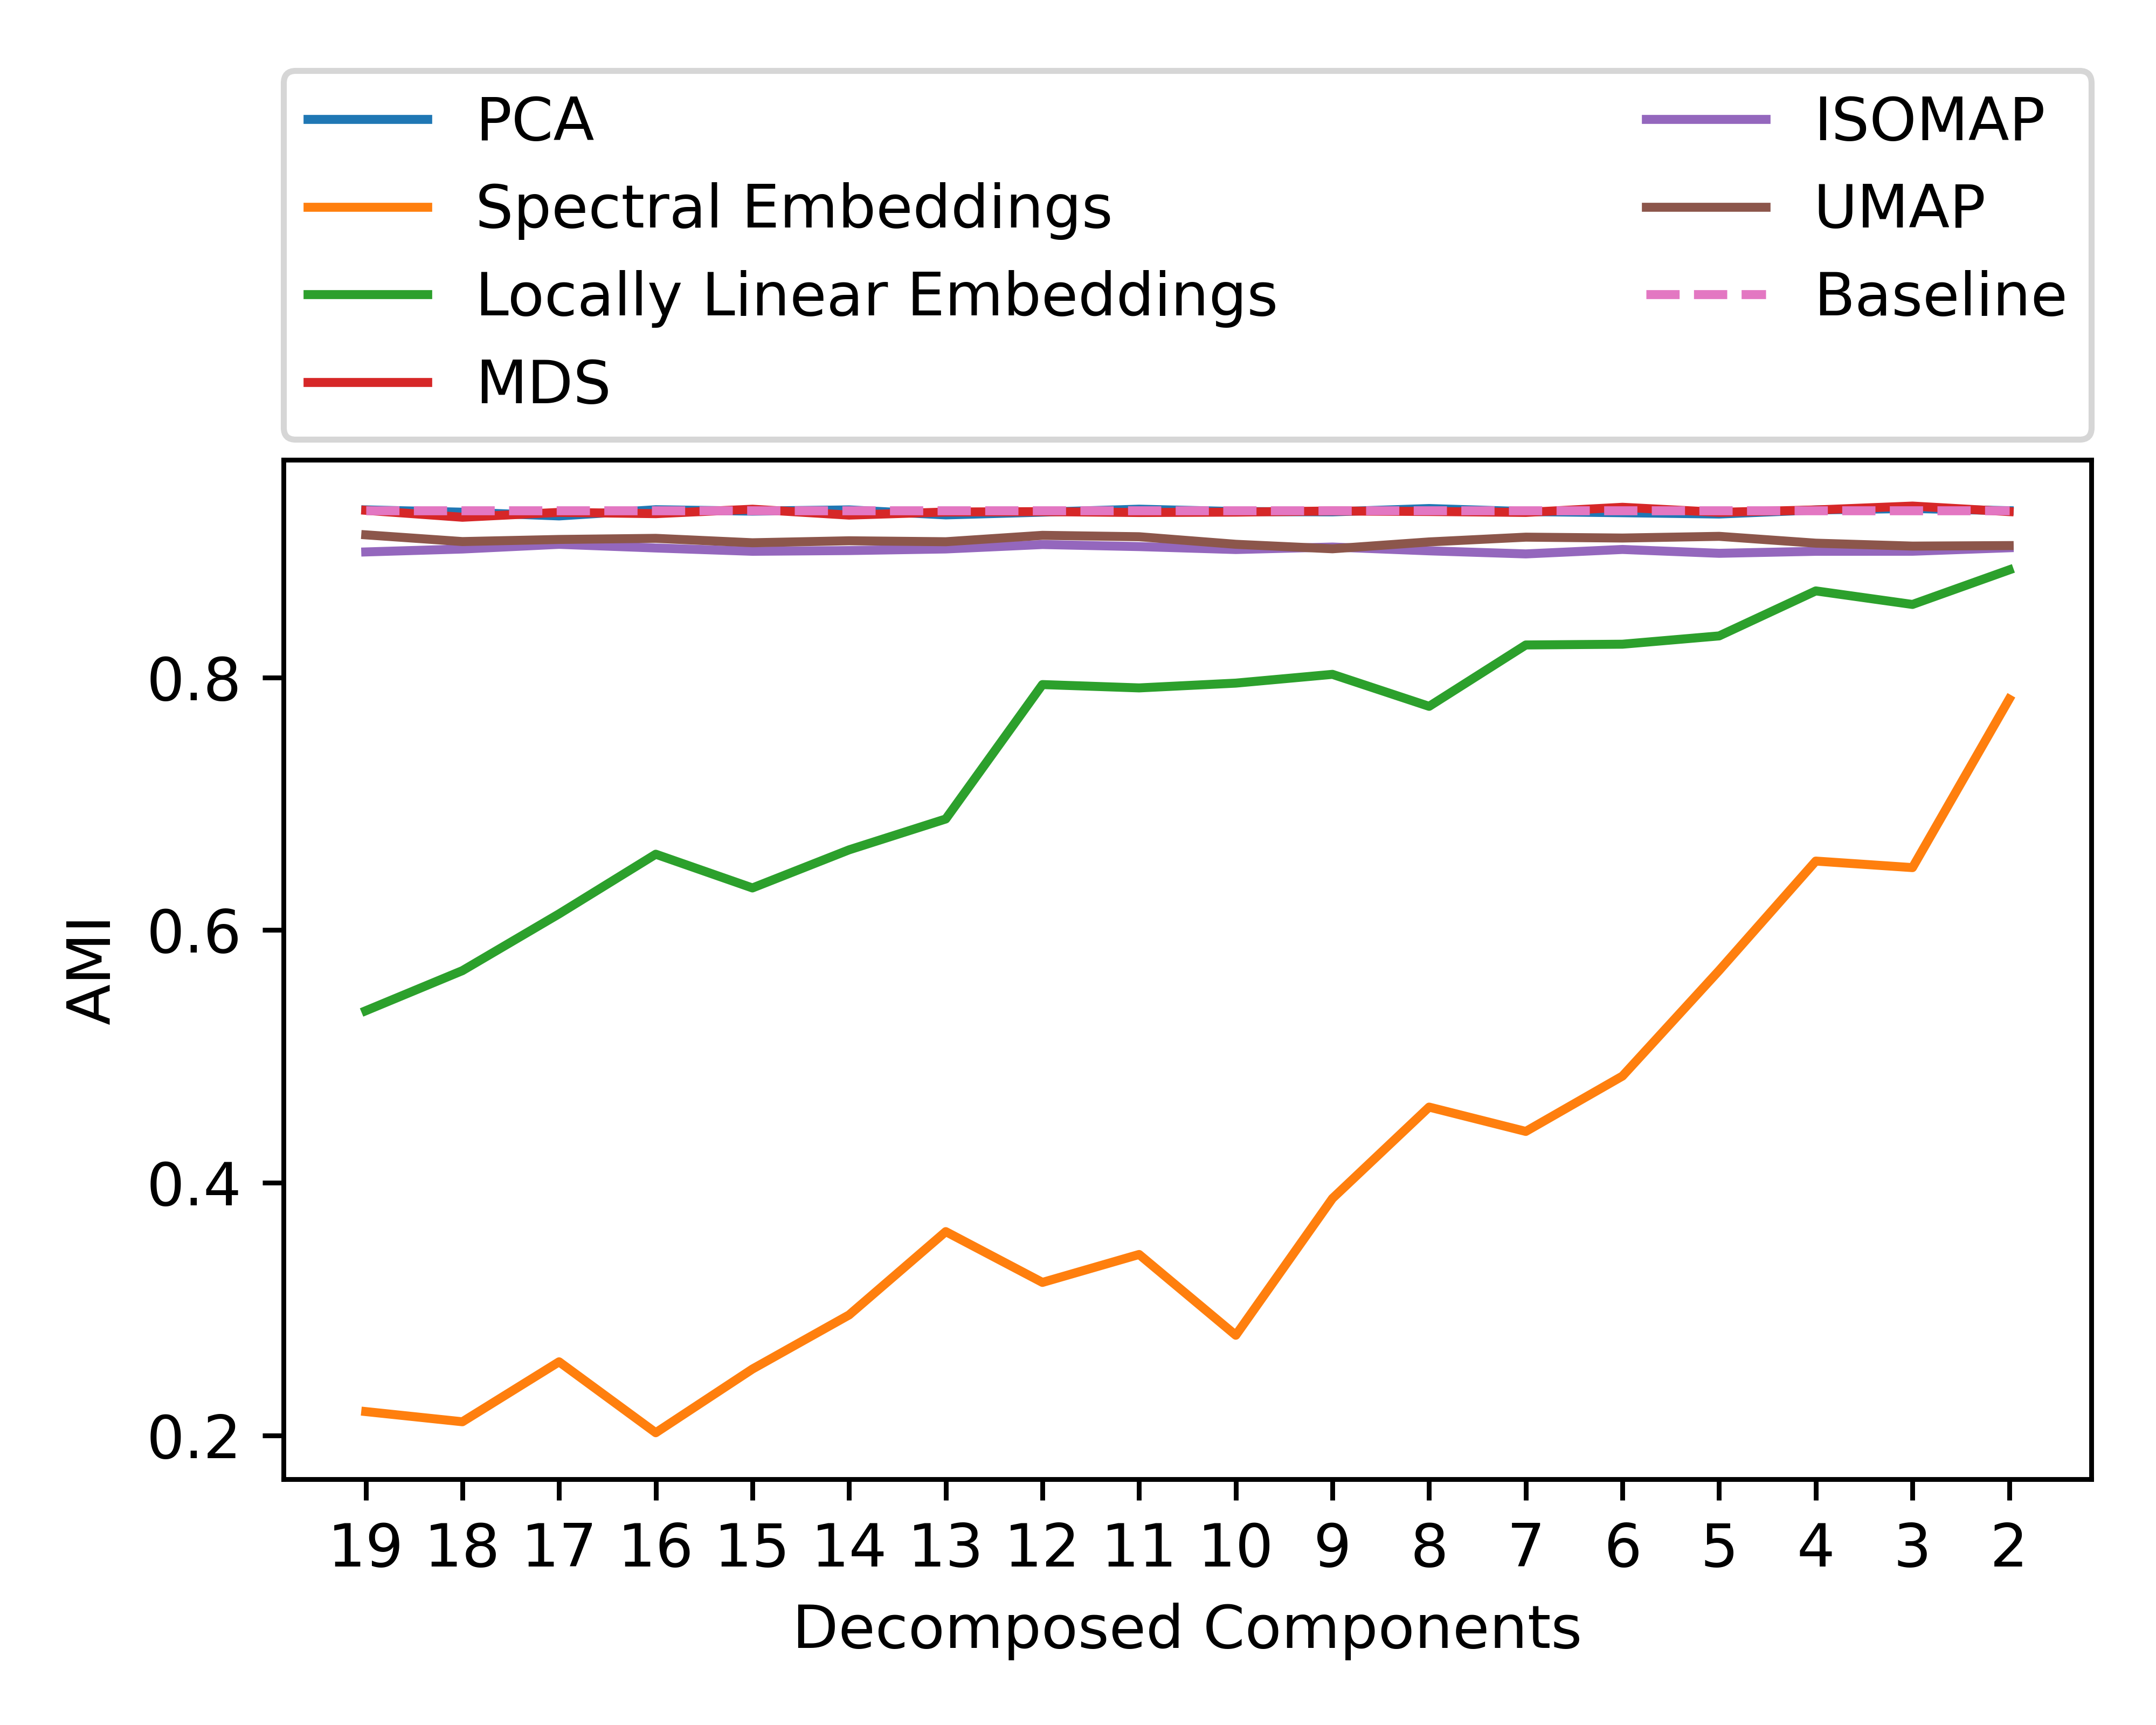
\includegraphics[width=0.48\linewidth]{images/charts/detailed_decomposition_metric_t_0.4_p_2_comparison_2_clusters_ami.png}
                        \label{subfig:synthetic:t_0.4:dim_influence:ami}
                    }
                    \subfigure[]{
                        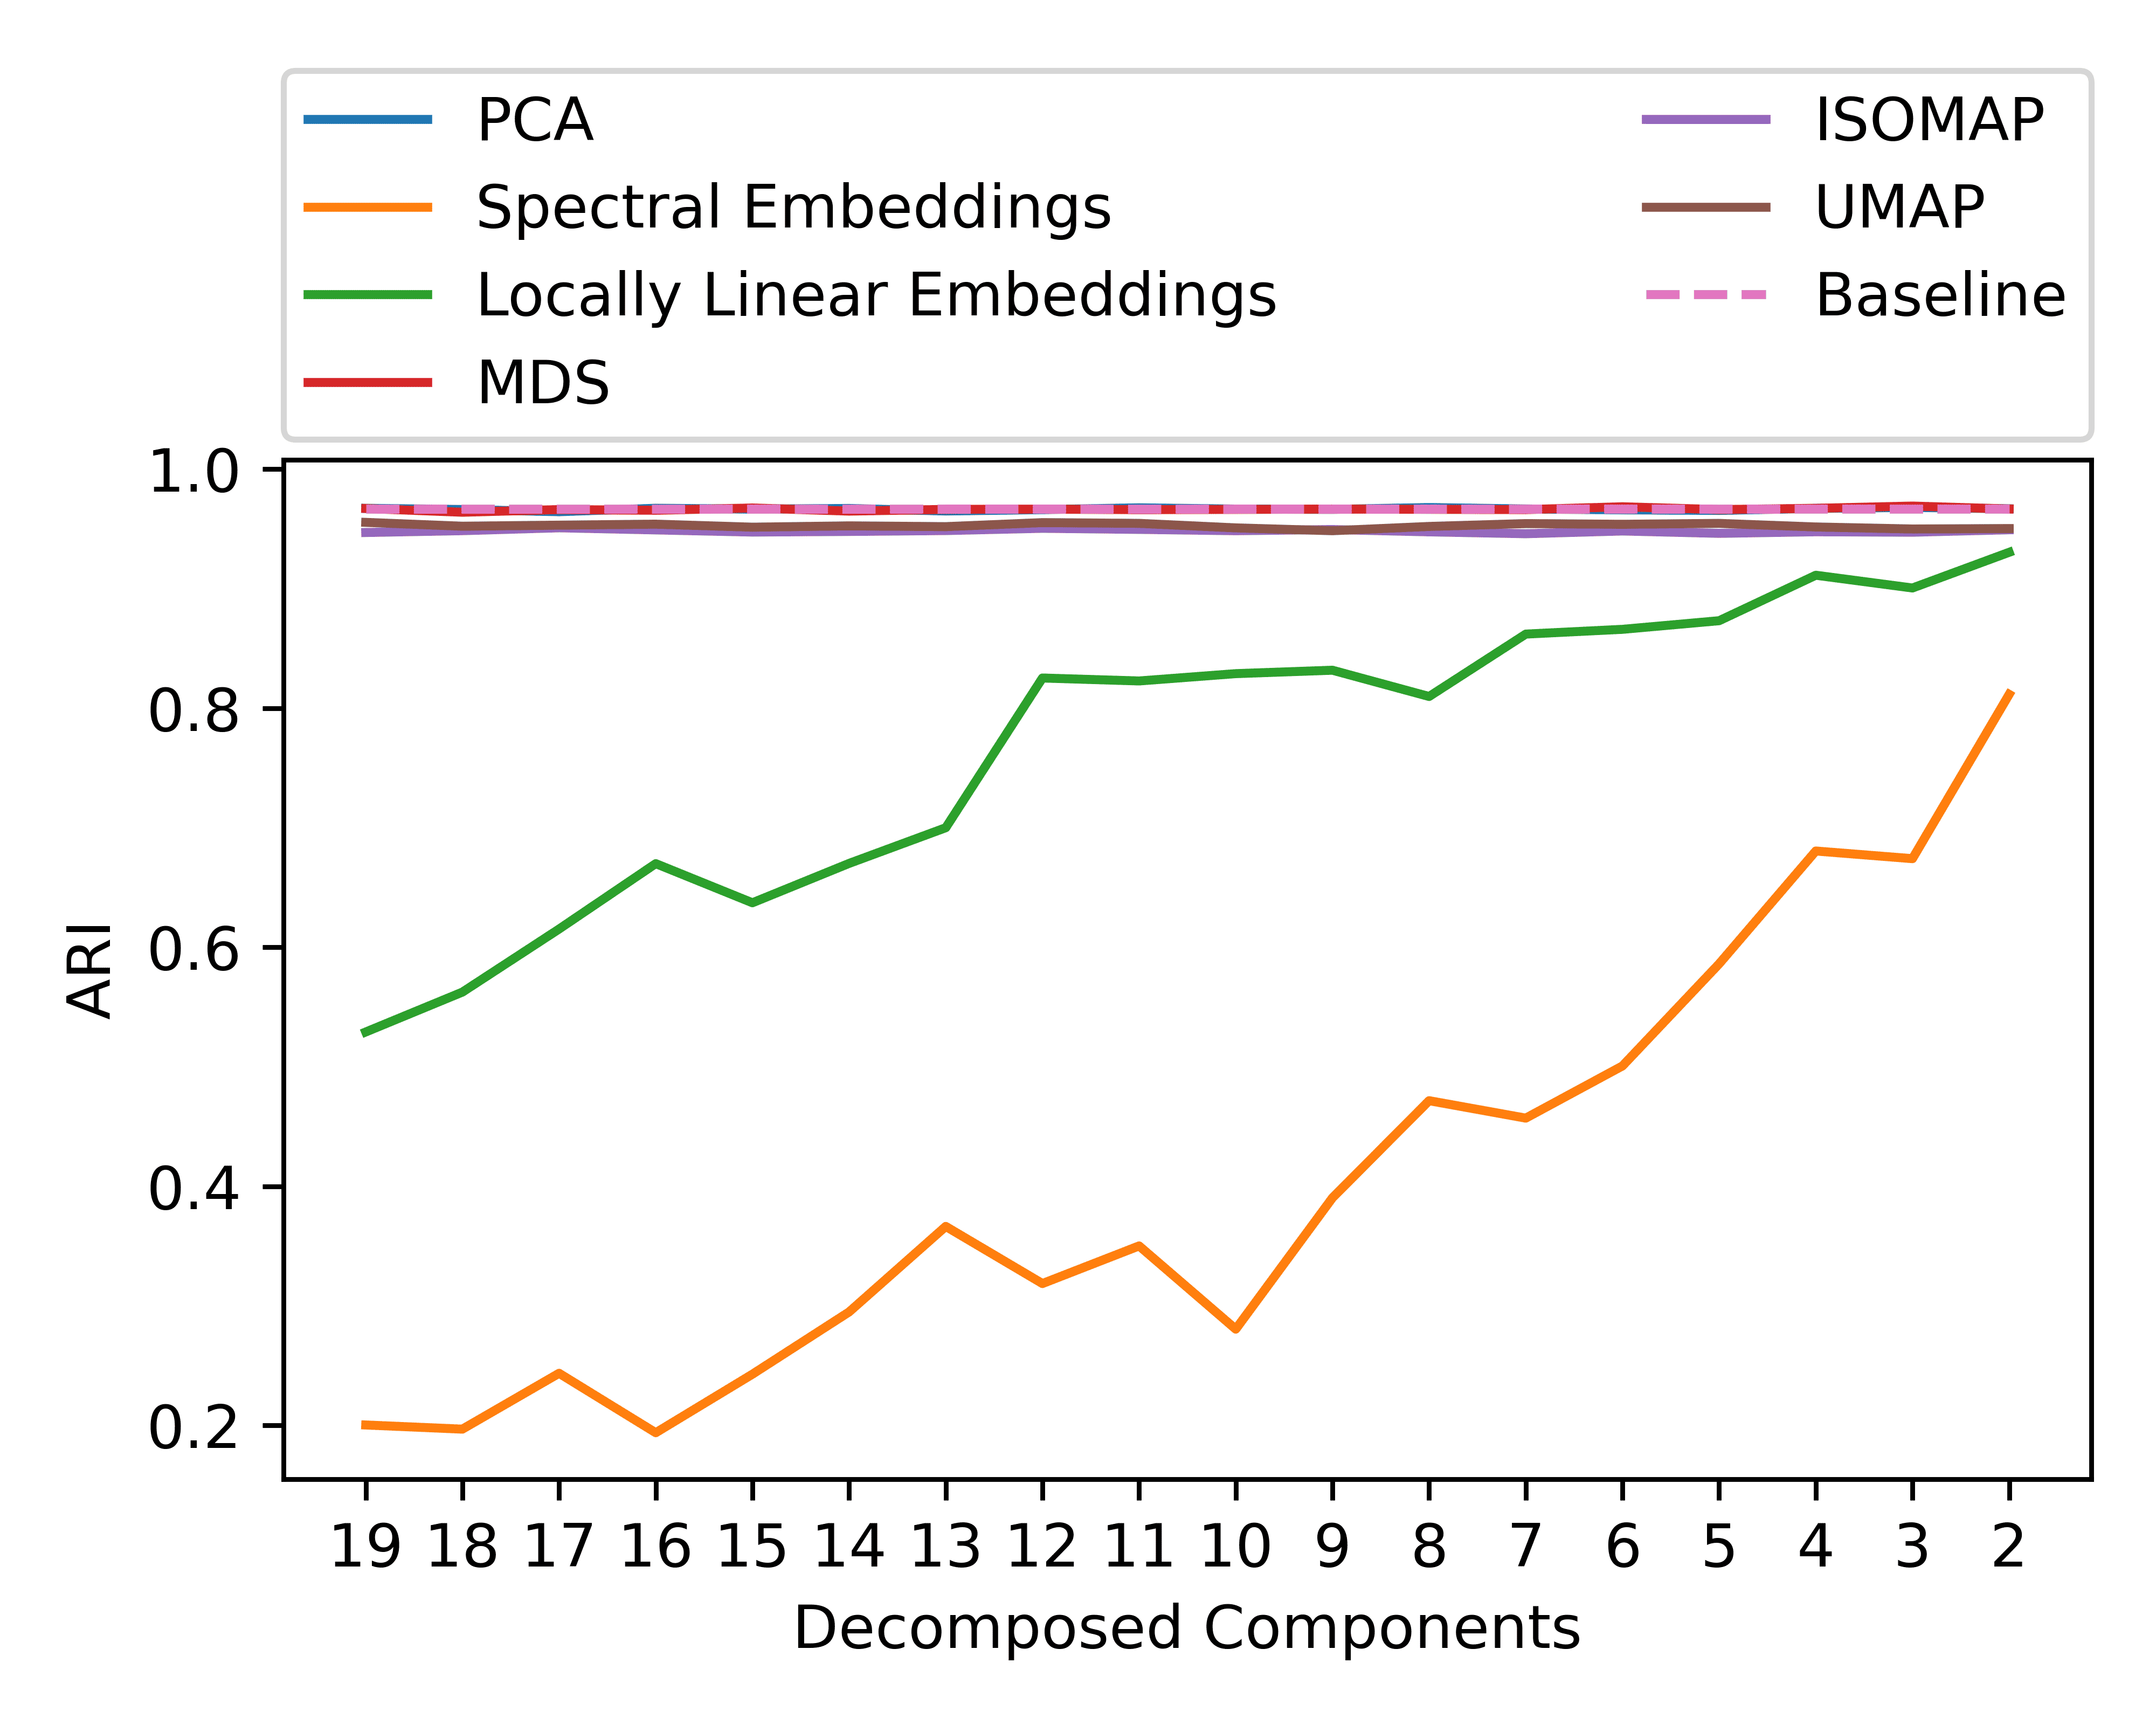
\includegraphics[width=0.48\linewidth]{images/charts/detailed_decomposition_metric_t_0.4_p_2_comparison_2_clusters_ari.png}
                        \label{subfig:synthetic:t_0.4:dim_influence:ari}
                    }
                    \subfigure[]{
                        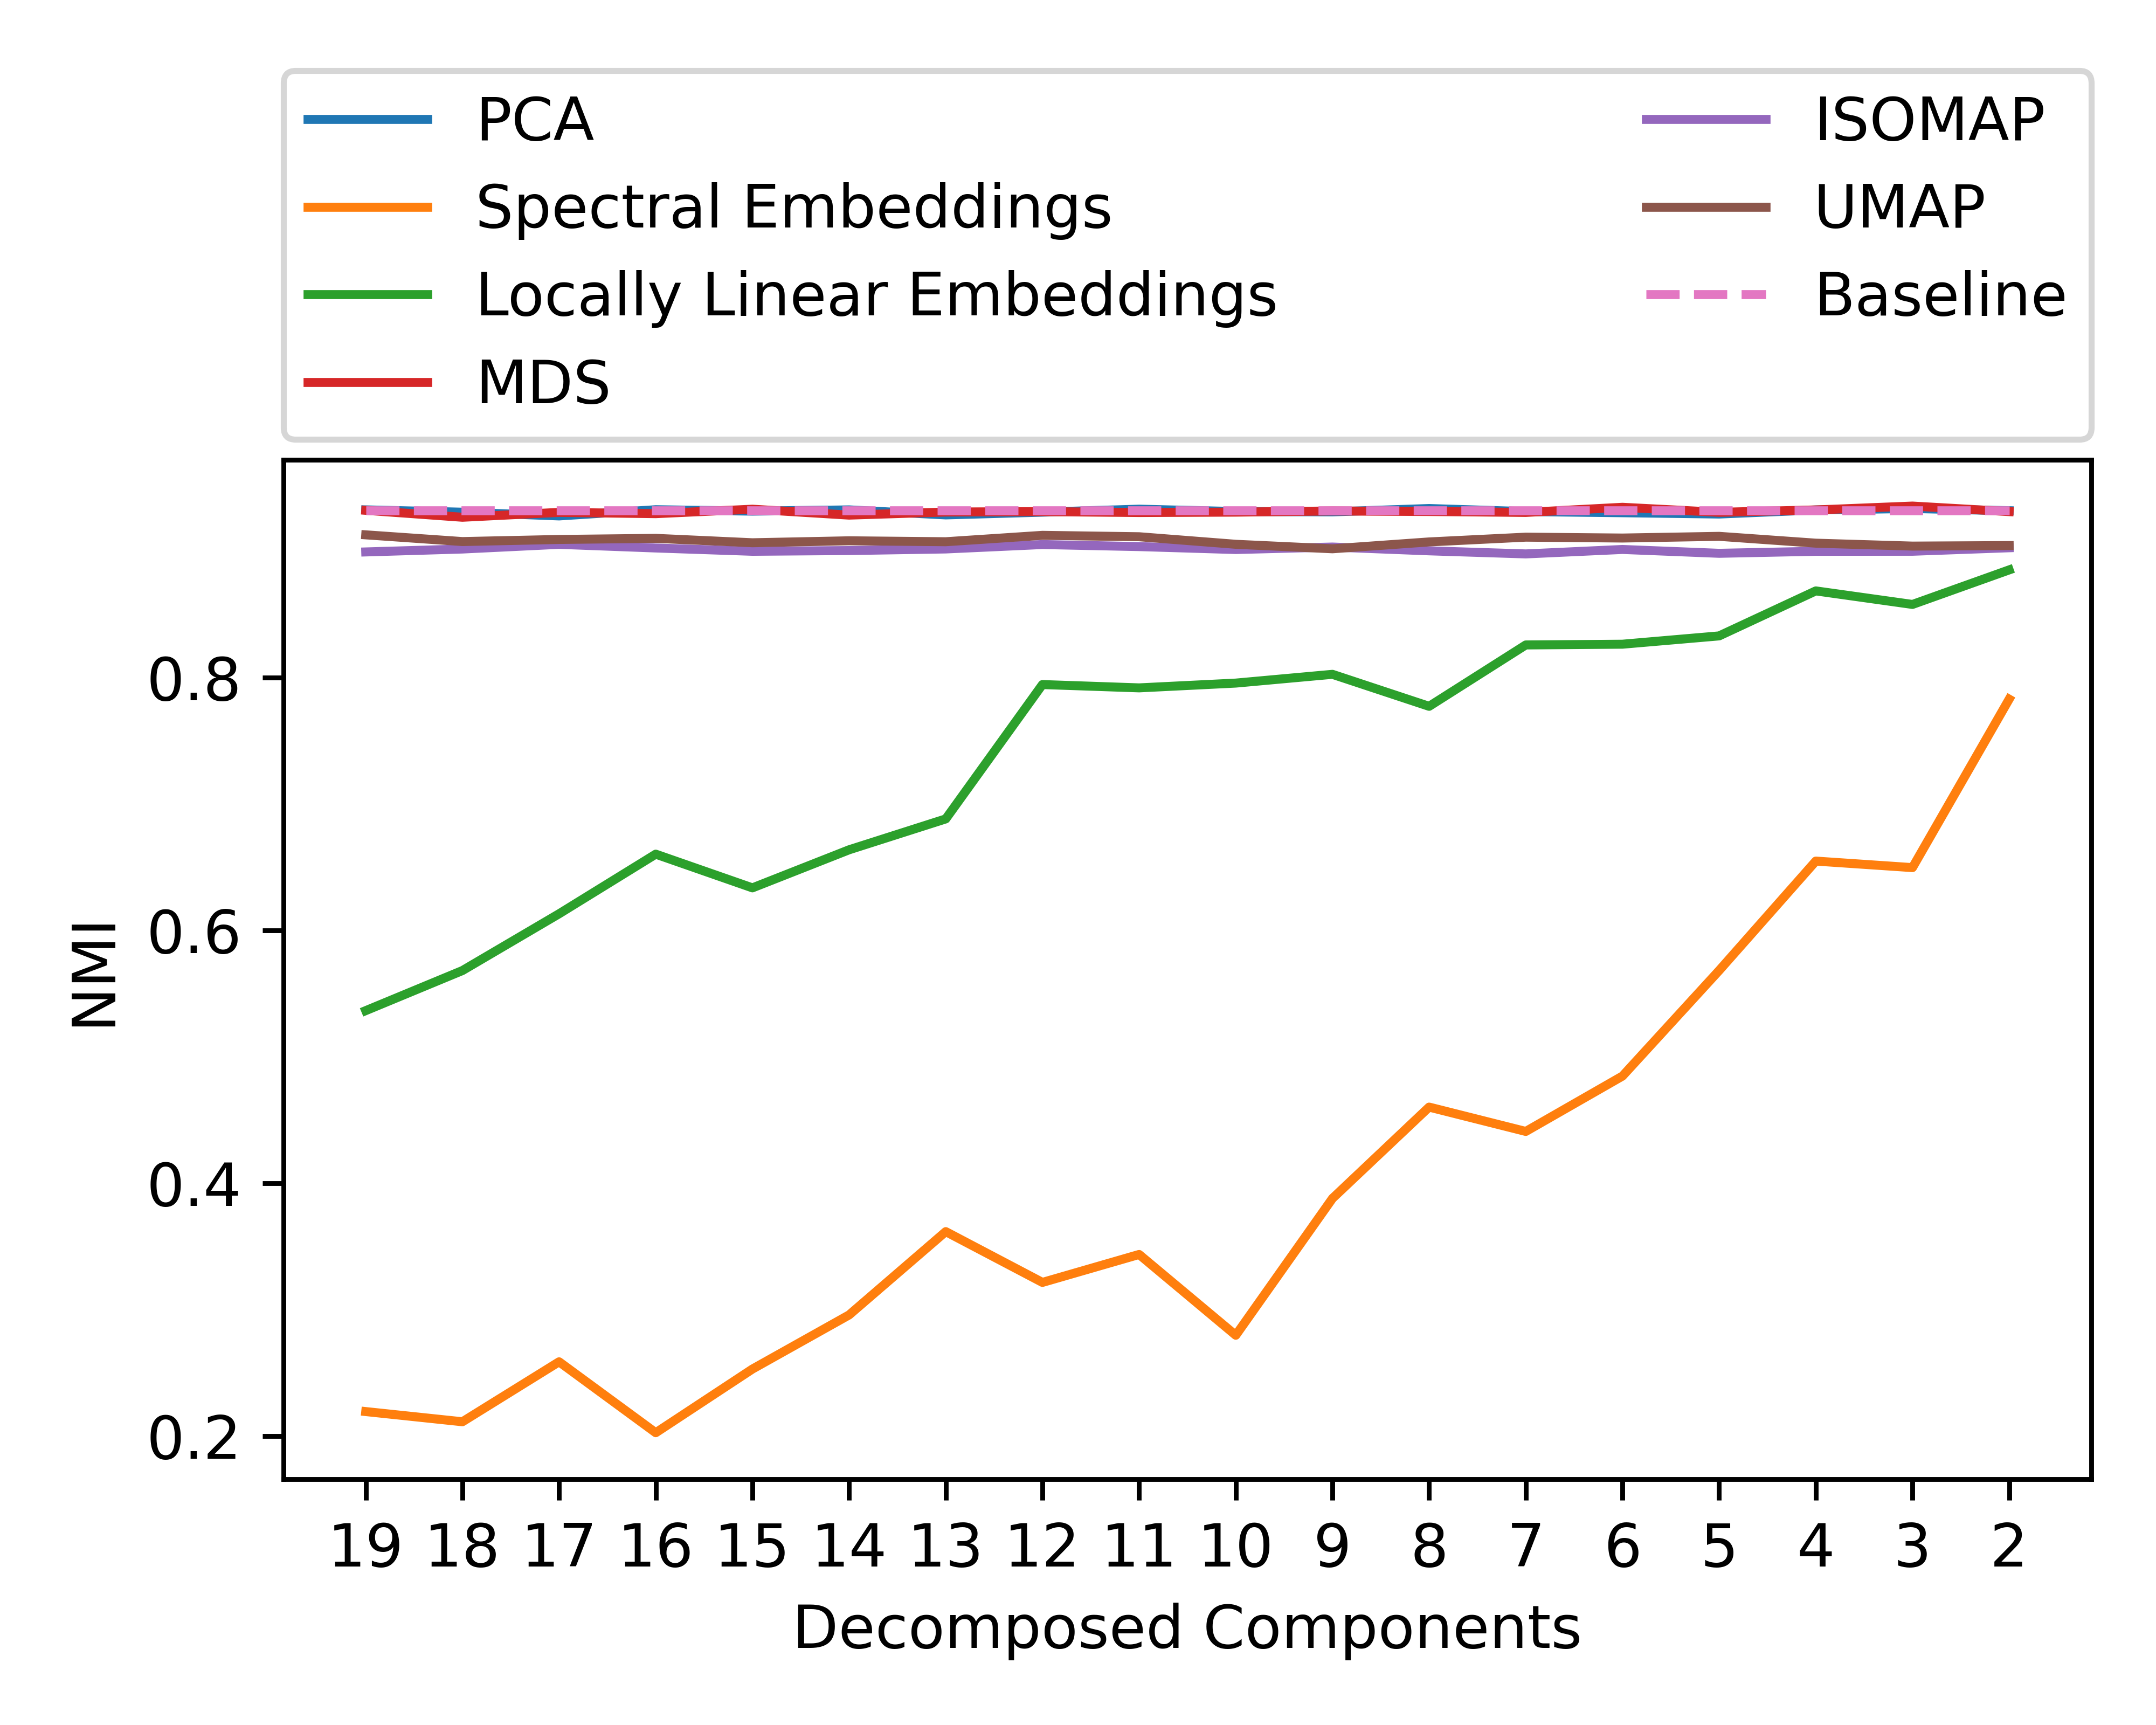
\includegraphics[width=0.48\linewidth]{images/charts/detailed_decomposition_metric_t_0.4_p_2_comparison_2_clusters_nmi.png}
                        \label{subfig:synthetic:t_0.4:dim_influence:nmi}
                    }
                    \subfigure[]{
                        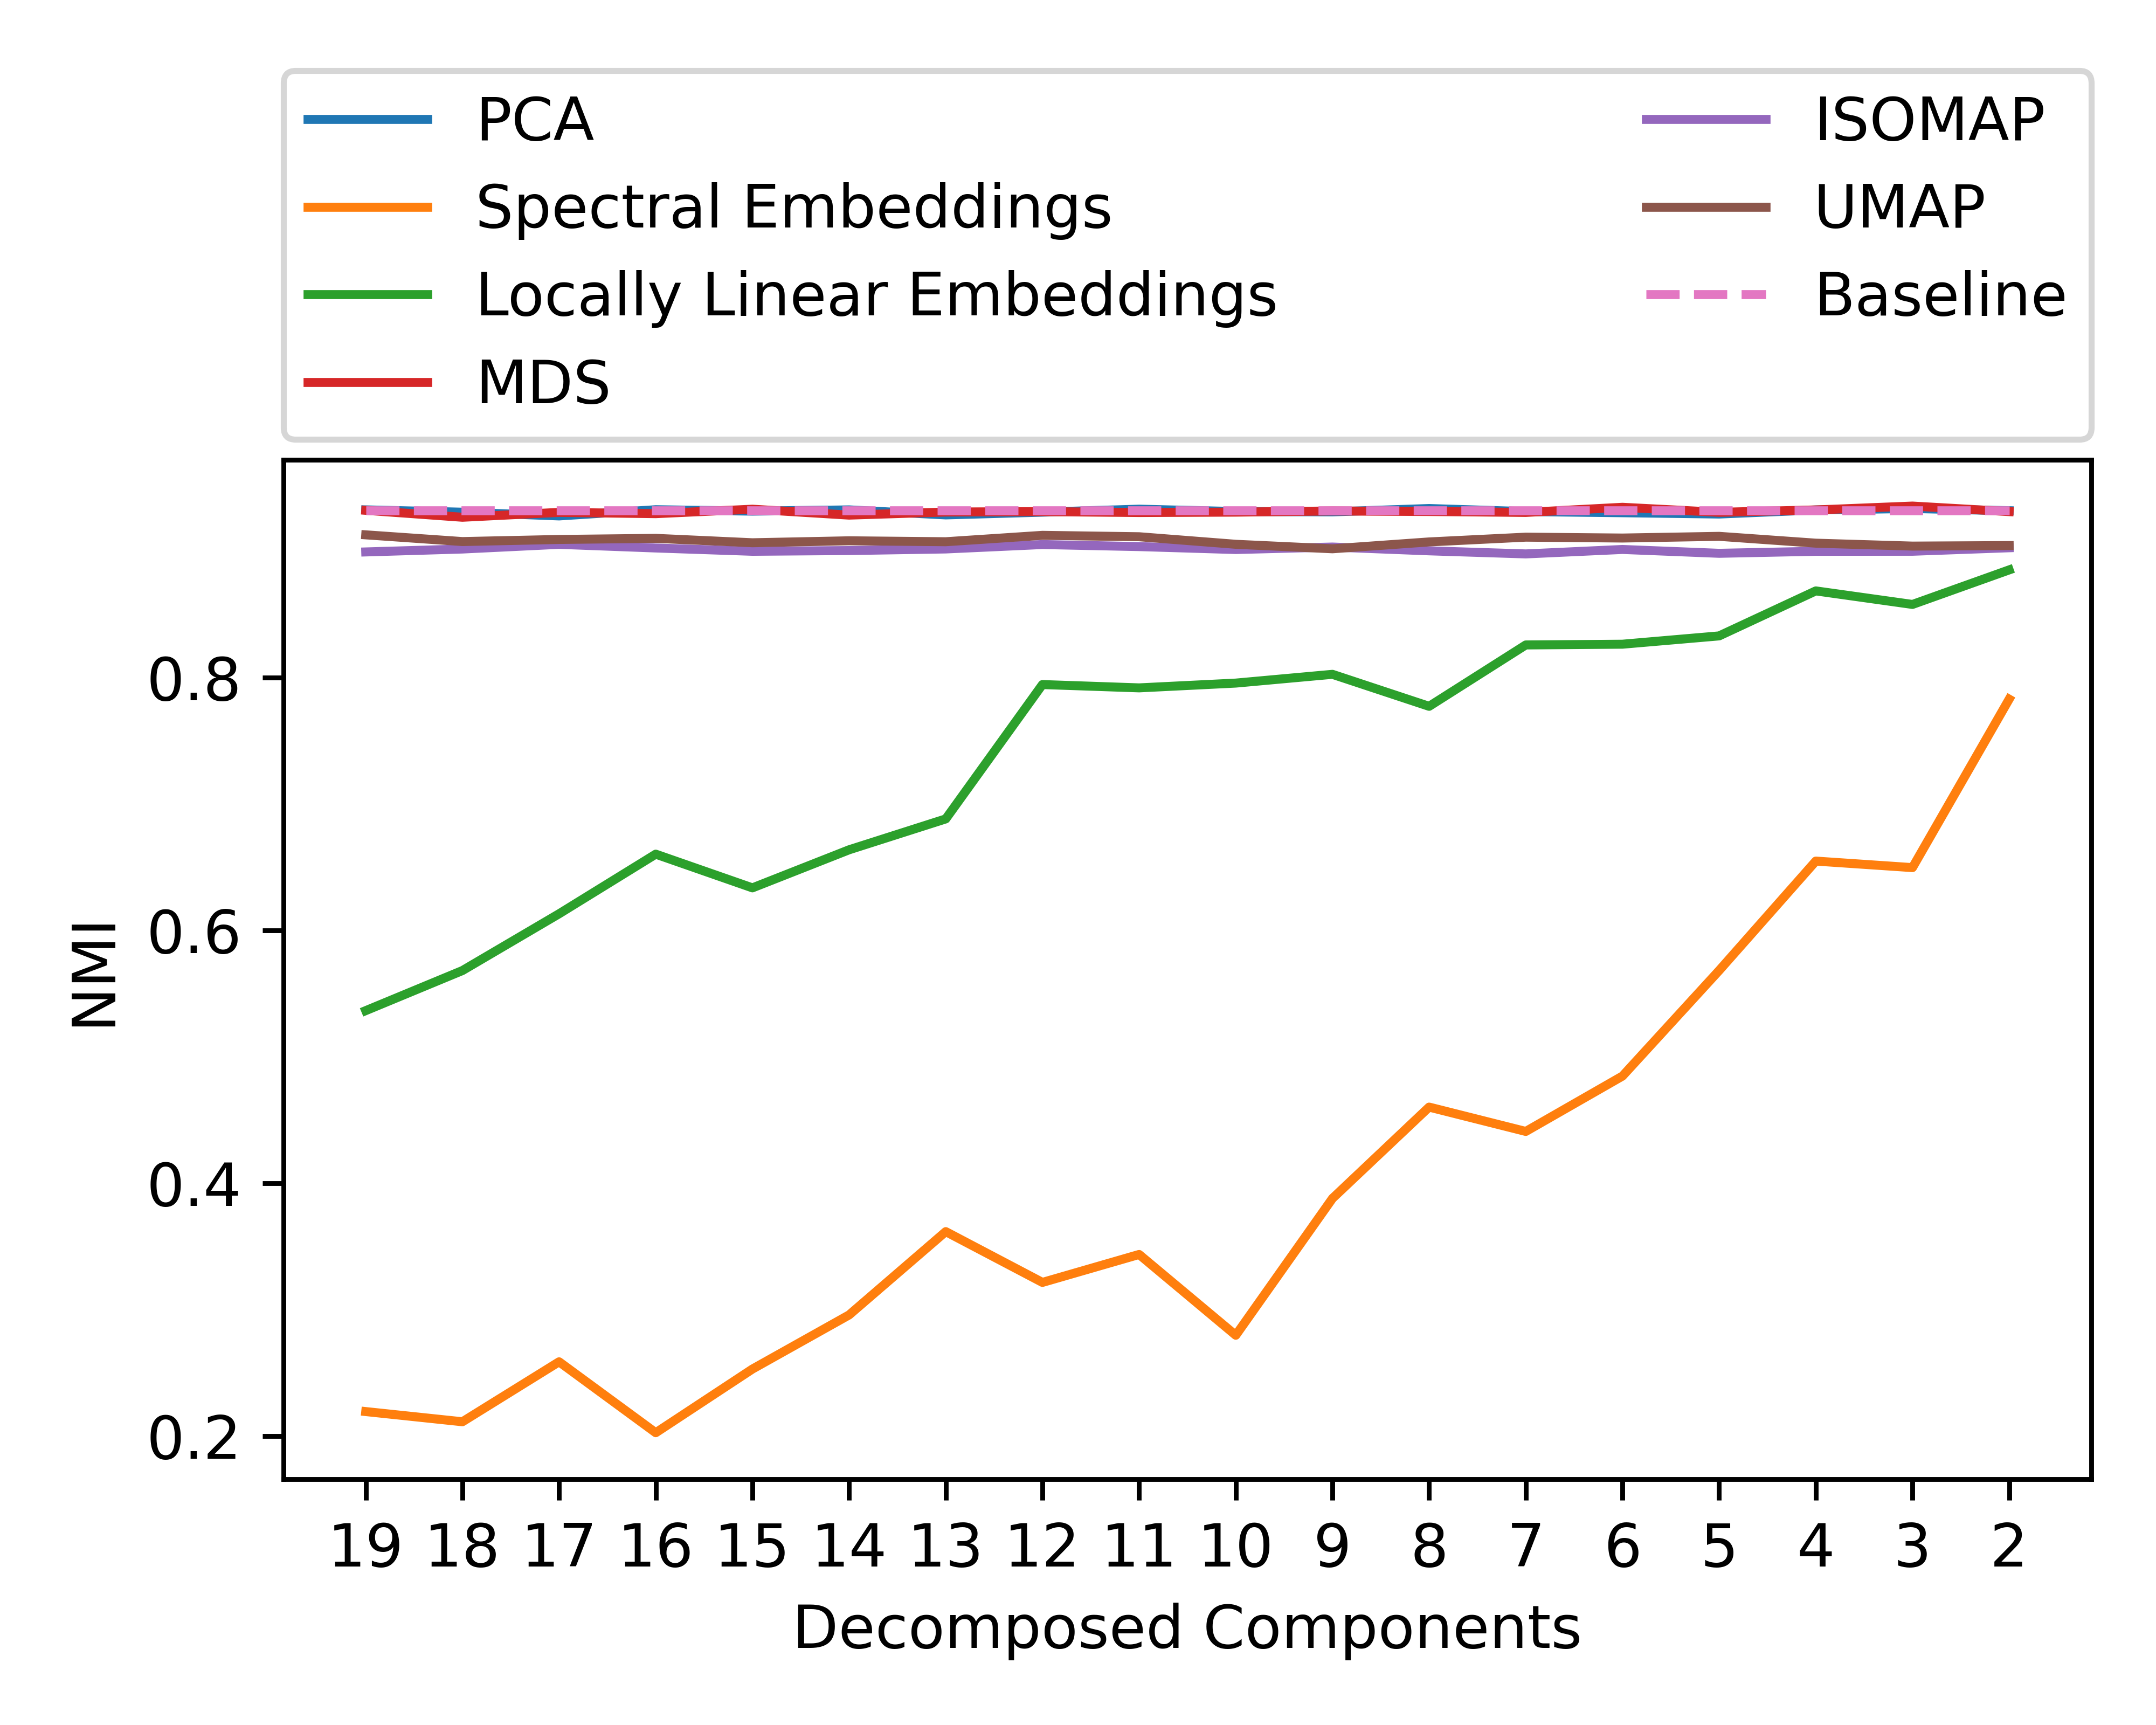
\includegraphics[width=0.48\linewidth]{images/charts/detailed_decomposition_metric_t_0.4_p_2_comparison_2_clusters_nmi.png}
                        \label{subfig:synthetic:t_0.4:dim_influence:time}
                    }
                    \caption{Анализ влияния размерности данных при различных методах снижения размерности на кластеризацию синтетического набора данных с параметром \(t = 0.4\). Результаты для
                        \subref{subfig:synthetic:t_0.4:dim_influence:ami} AMI;
                        \subref{subfig:synthetic:t_0.4:dim_influence:ari} ARI;
                        \subref{subfig:synthetic:t_0.4:dim_influence:nmi} NMI, а также на время работы алгоритма \subref{subfig:synthetic:t_influence:time}.
                    }
                    \label{fig:synthetic:t_0.4:dim_influence}
                \end{figure}

                \begin{figure}[H]\centering
                    \subfigure[]{
                        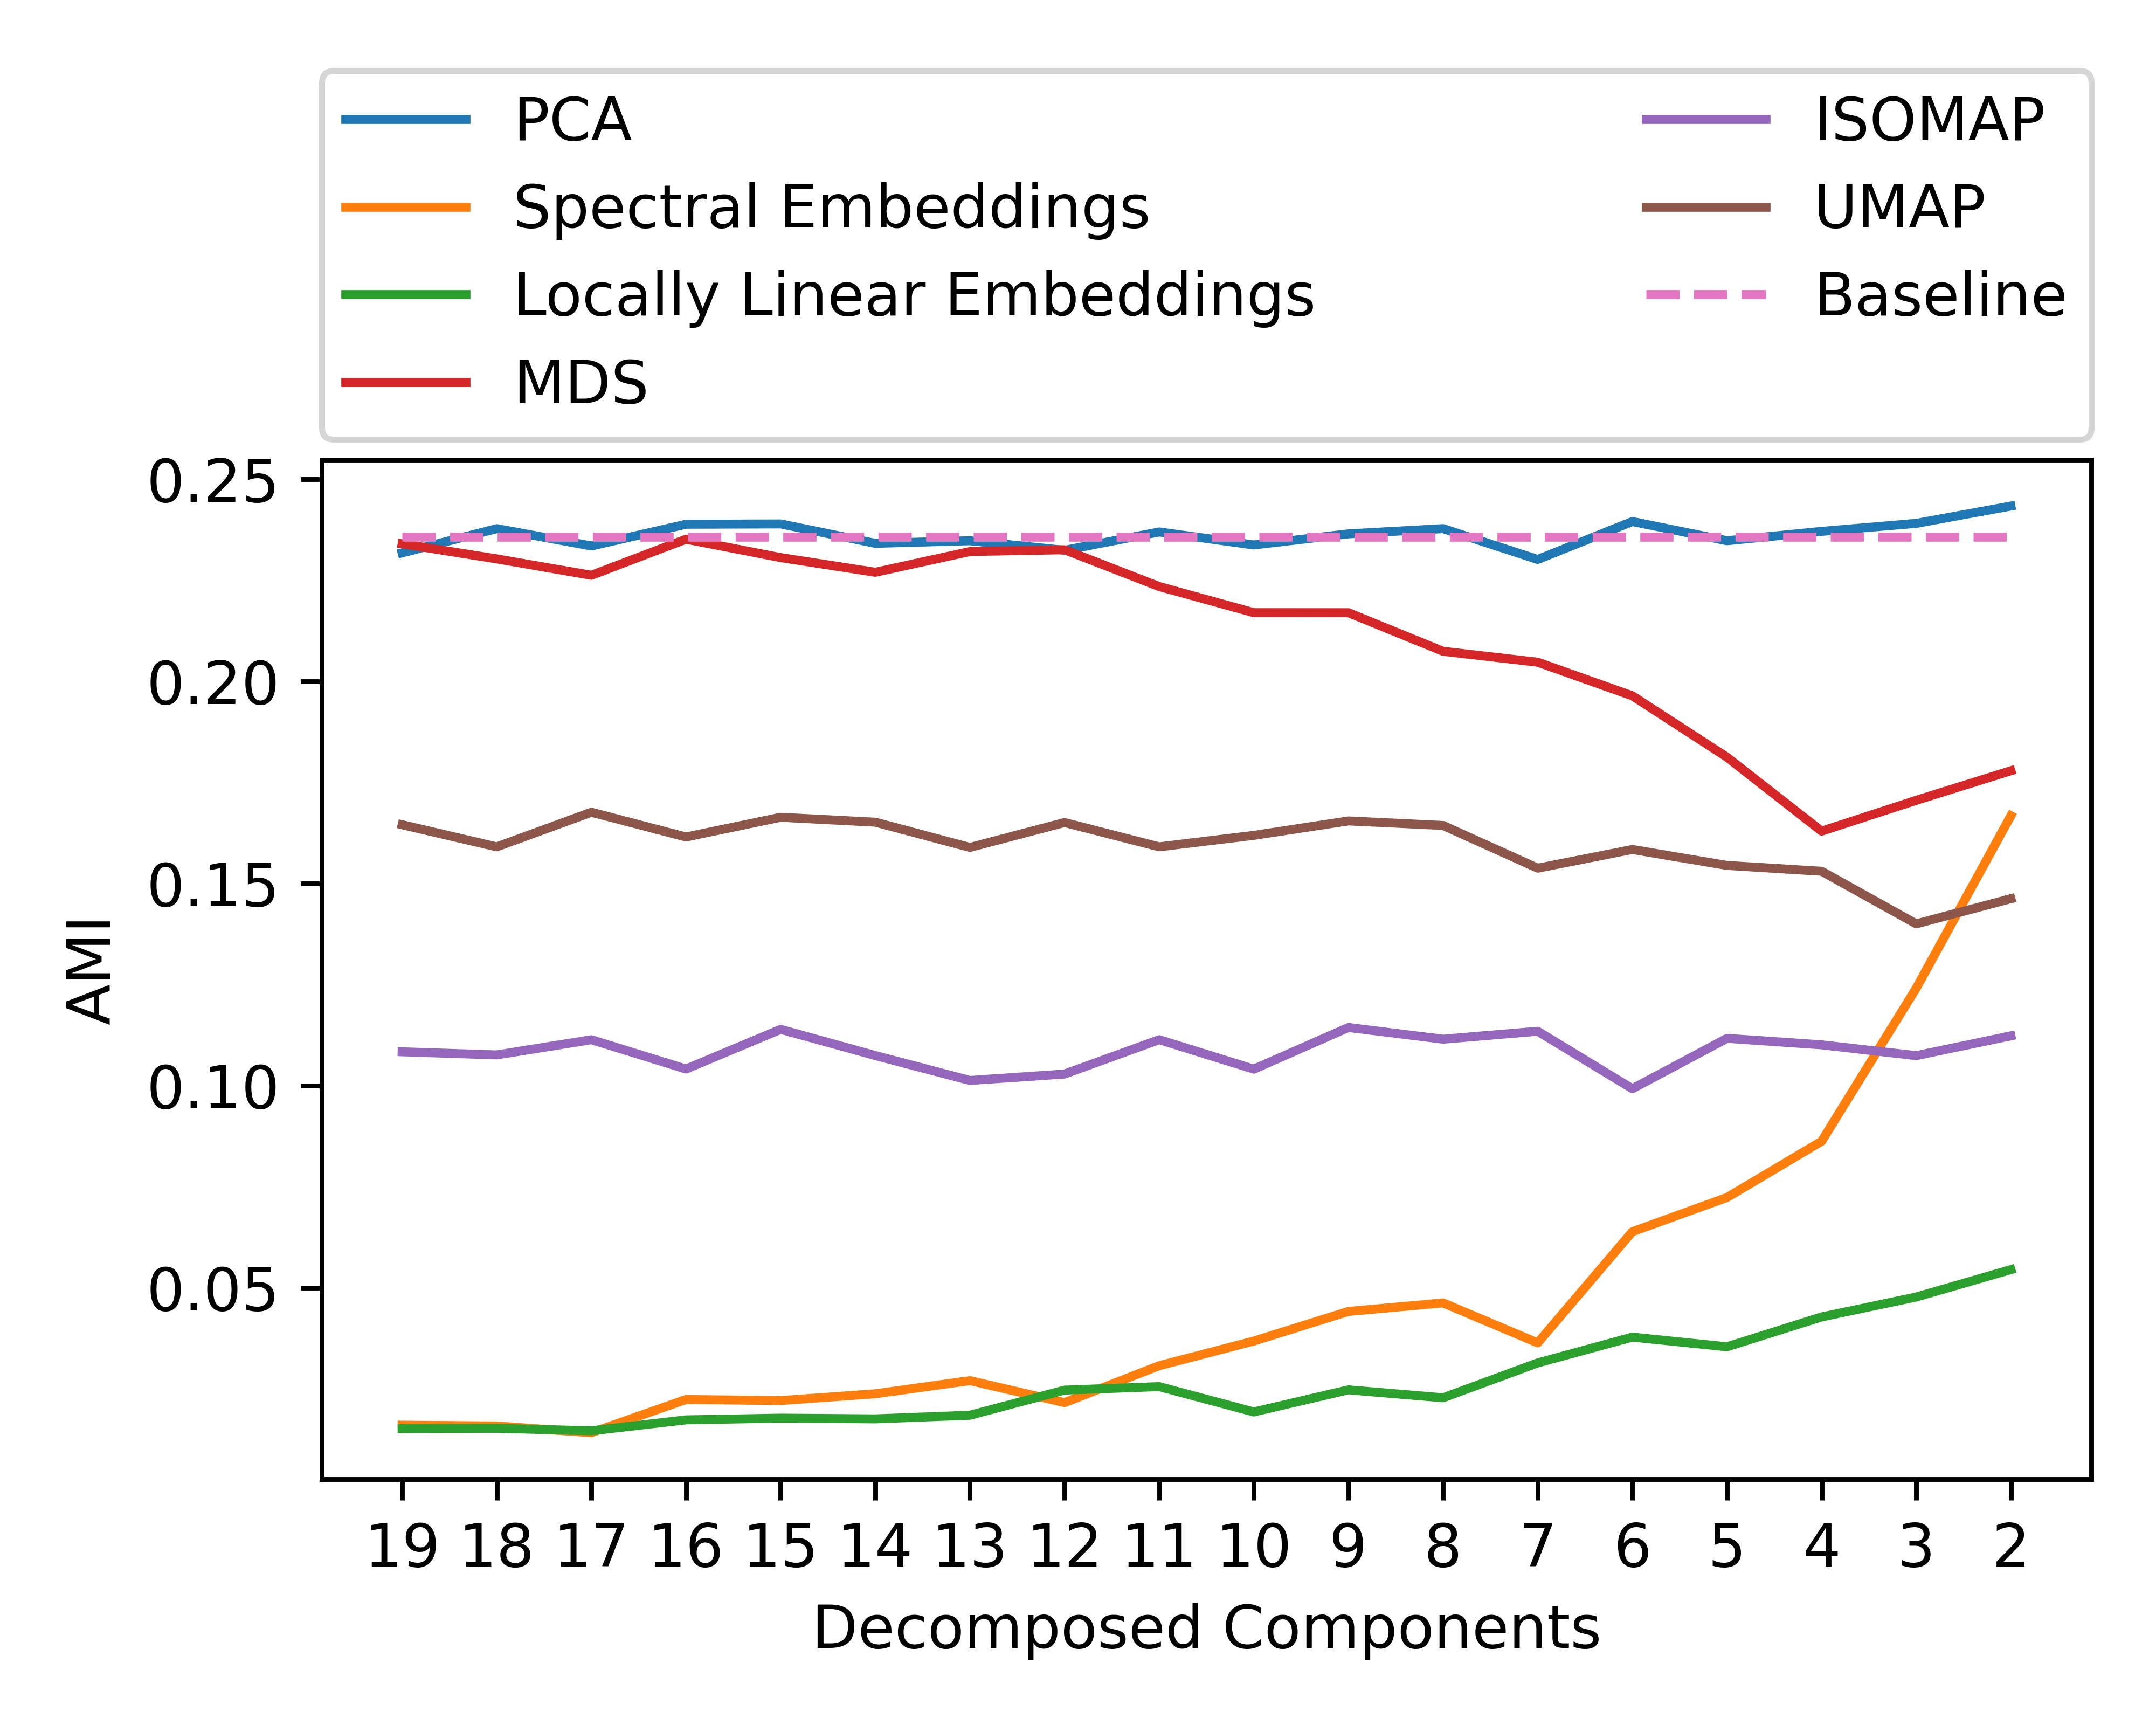
\includegraphics[width=0.48\linewidth]{images/charts/detailed_decomposition_metric_t_0.8_p_2_comparison_2_clusters_ami.png}
                        \label{subfig:synthetic:t_0.8:dim_influence:ami}
                    }
                    \subfigure[]{
                        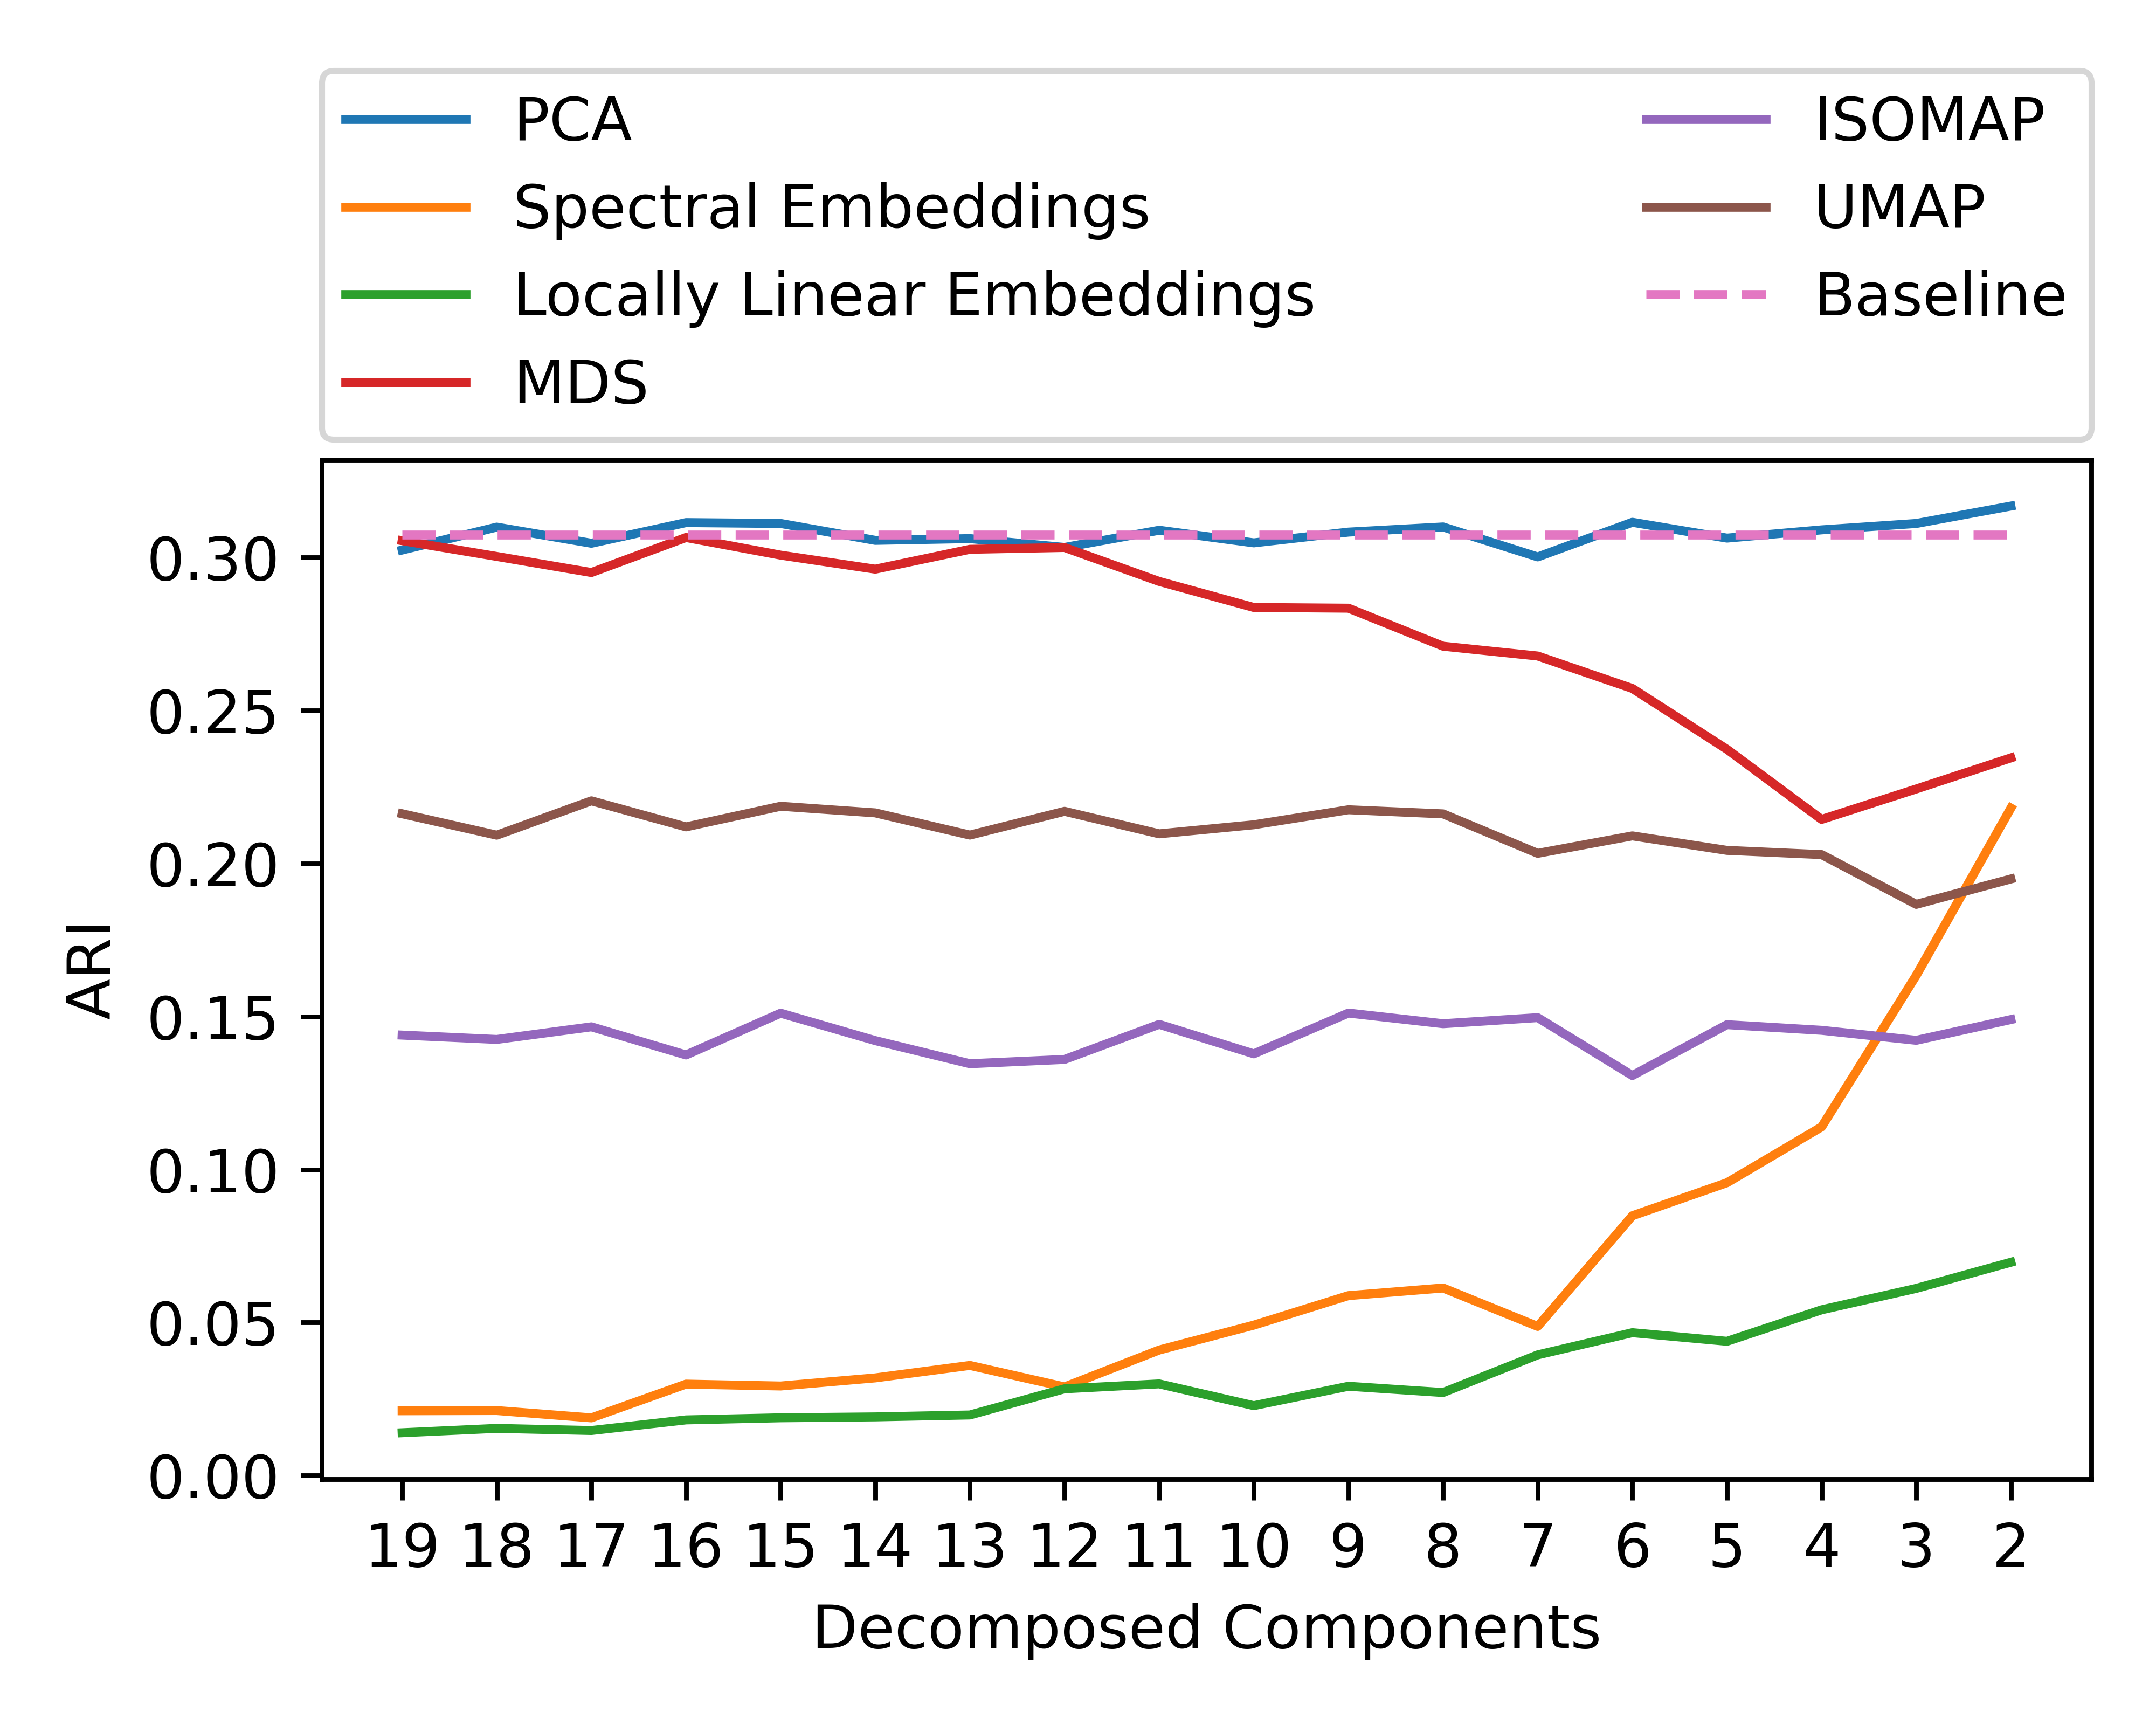
\includegraphics[width=0.48\linewidth]{images/charts/detailed_decomposition_metric_t_0.8_p_2_comparison_2_clusters_ari.png}
                        \label{subfig:synthetic:t_0.8:dim_influence:ari}
                    }
                    \subfigure[]{
                        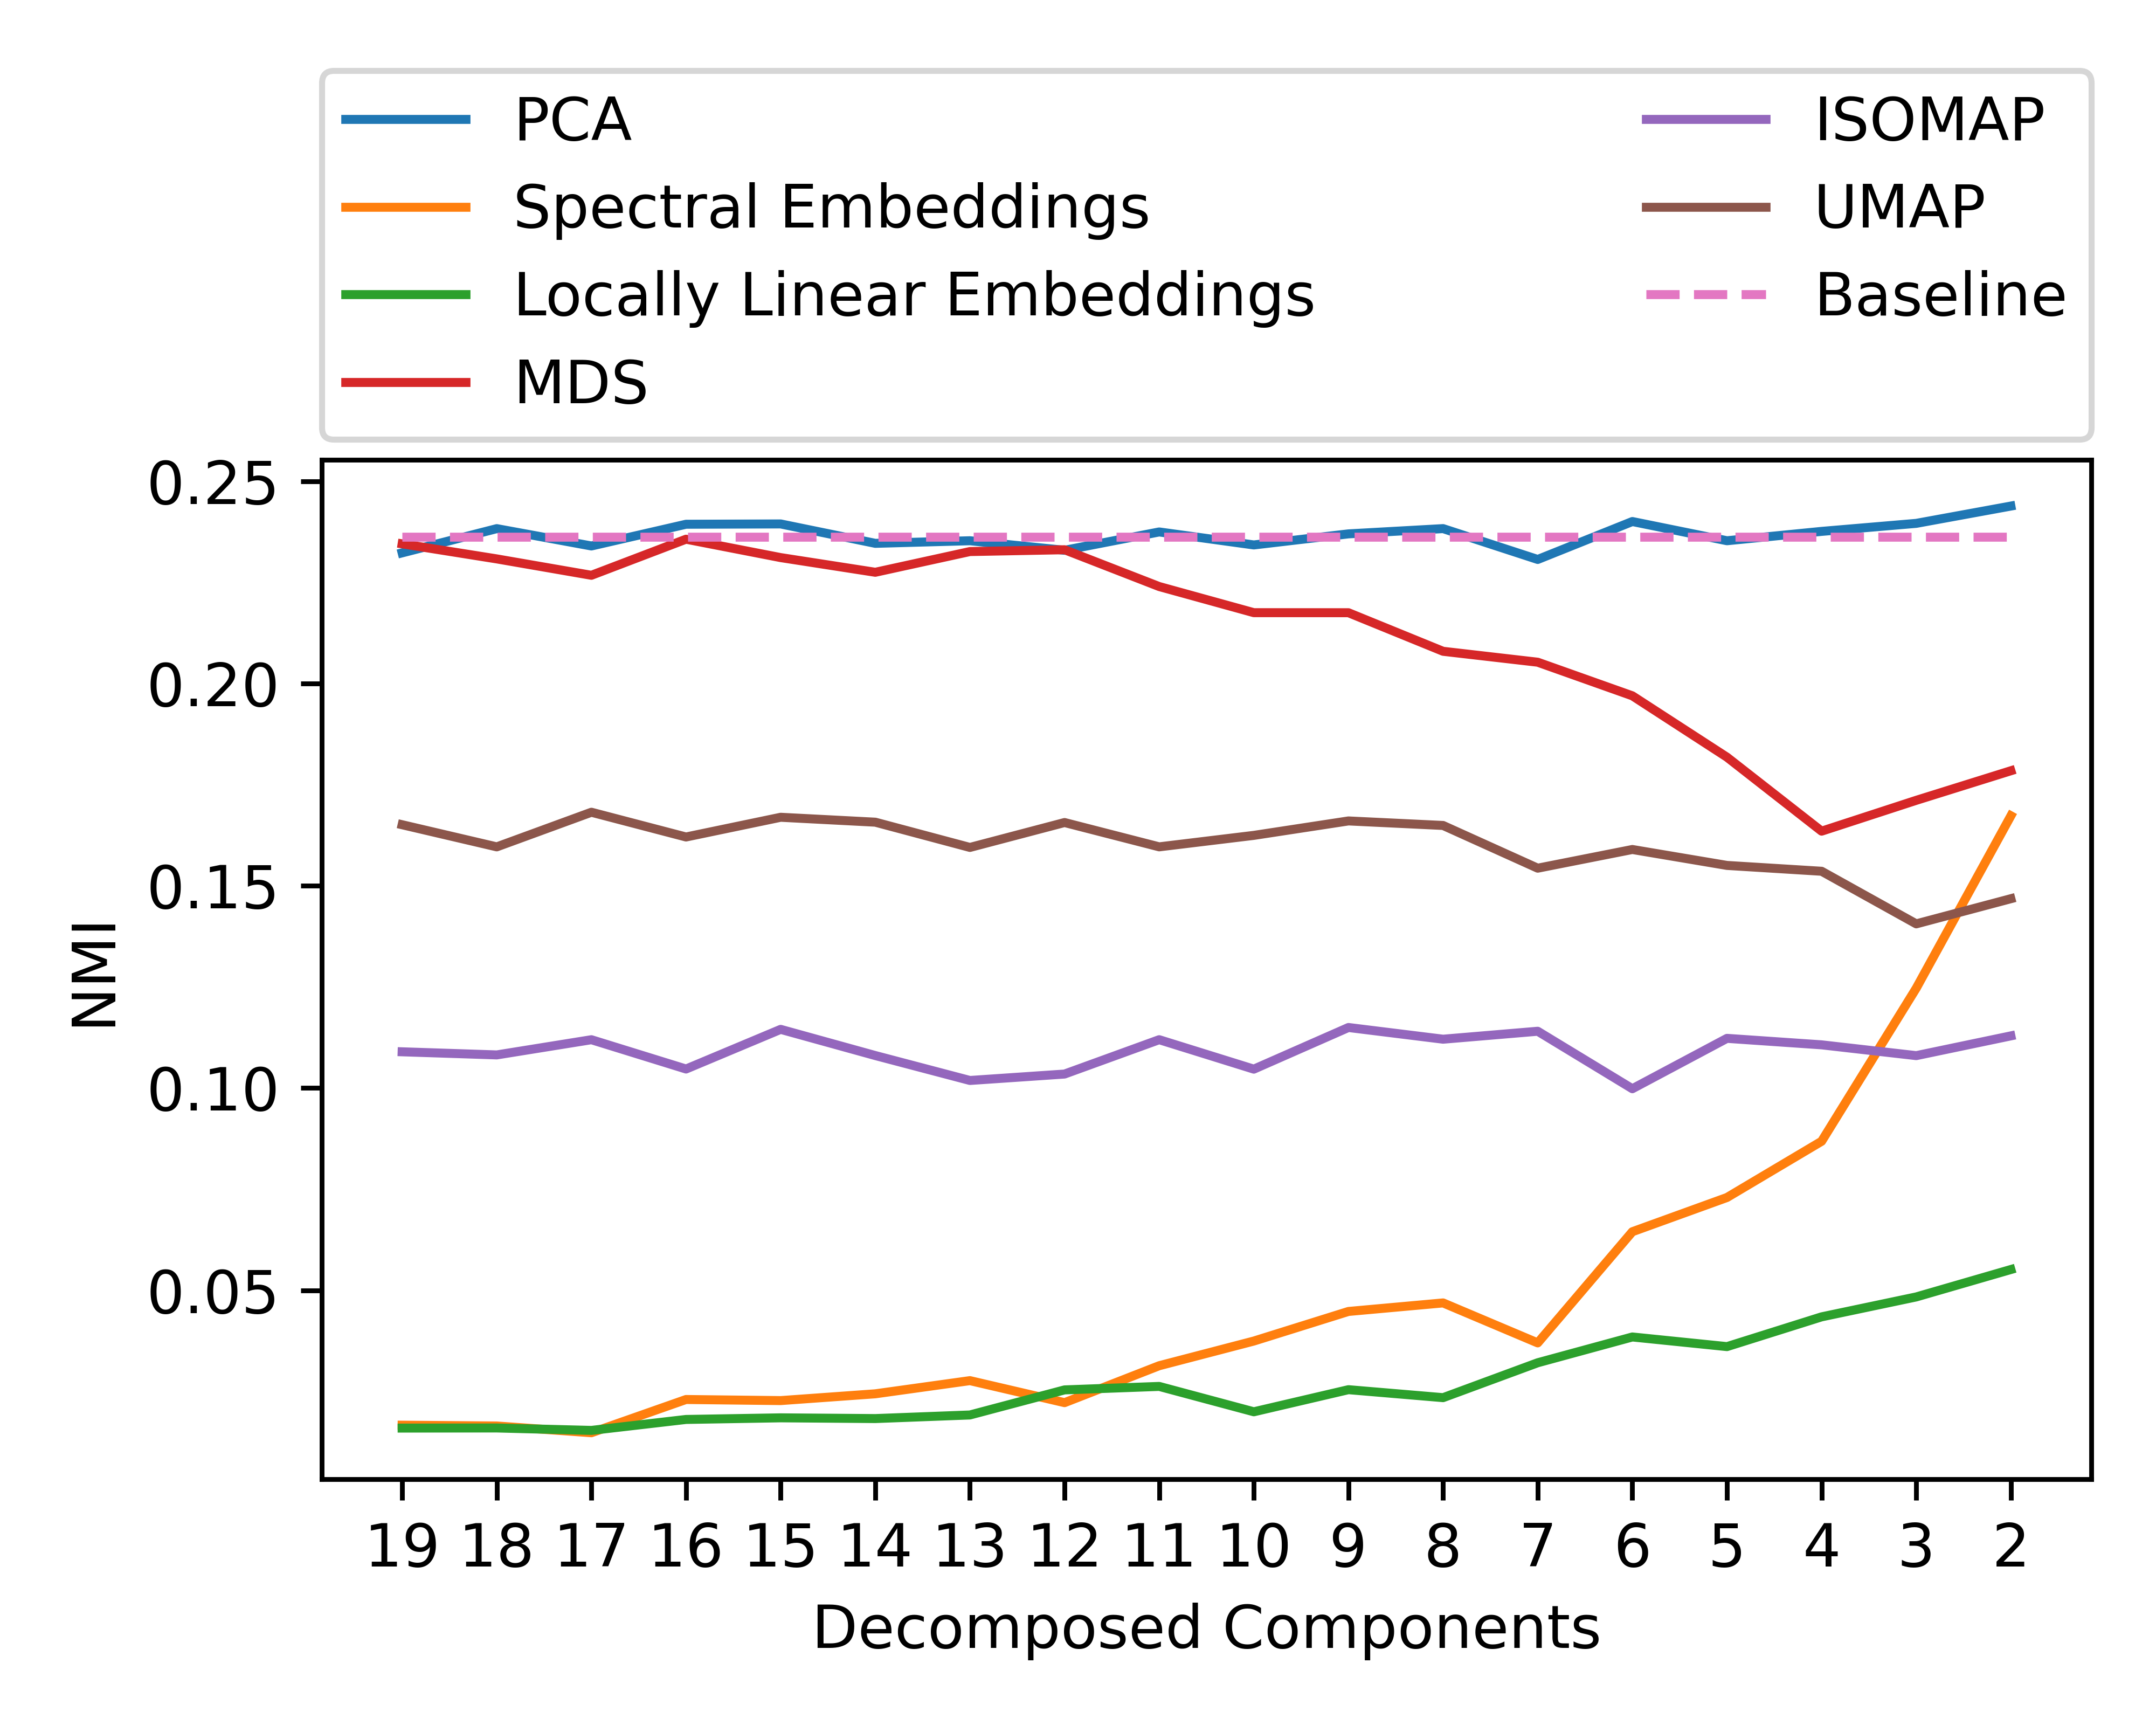
\includegraphics[width=0.48\linewidth]{images/charts/detailed_decomposition_metric_t_0.8_p_2_comparison_2_clusters_nmi.png}
                        \label{subfig:synthetic:t_0.8:dim_influence:nmi}
                    }
                    \subfigure[]{
                        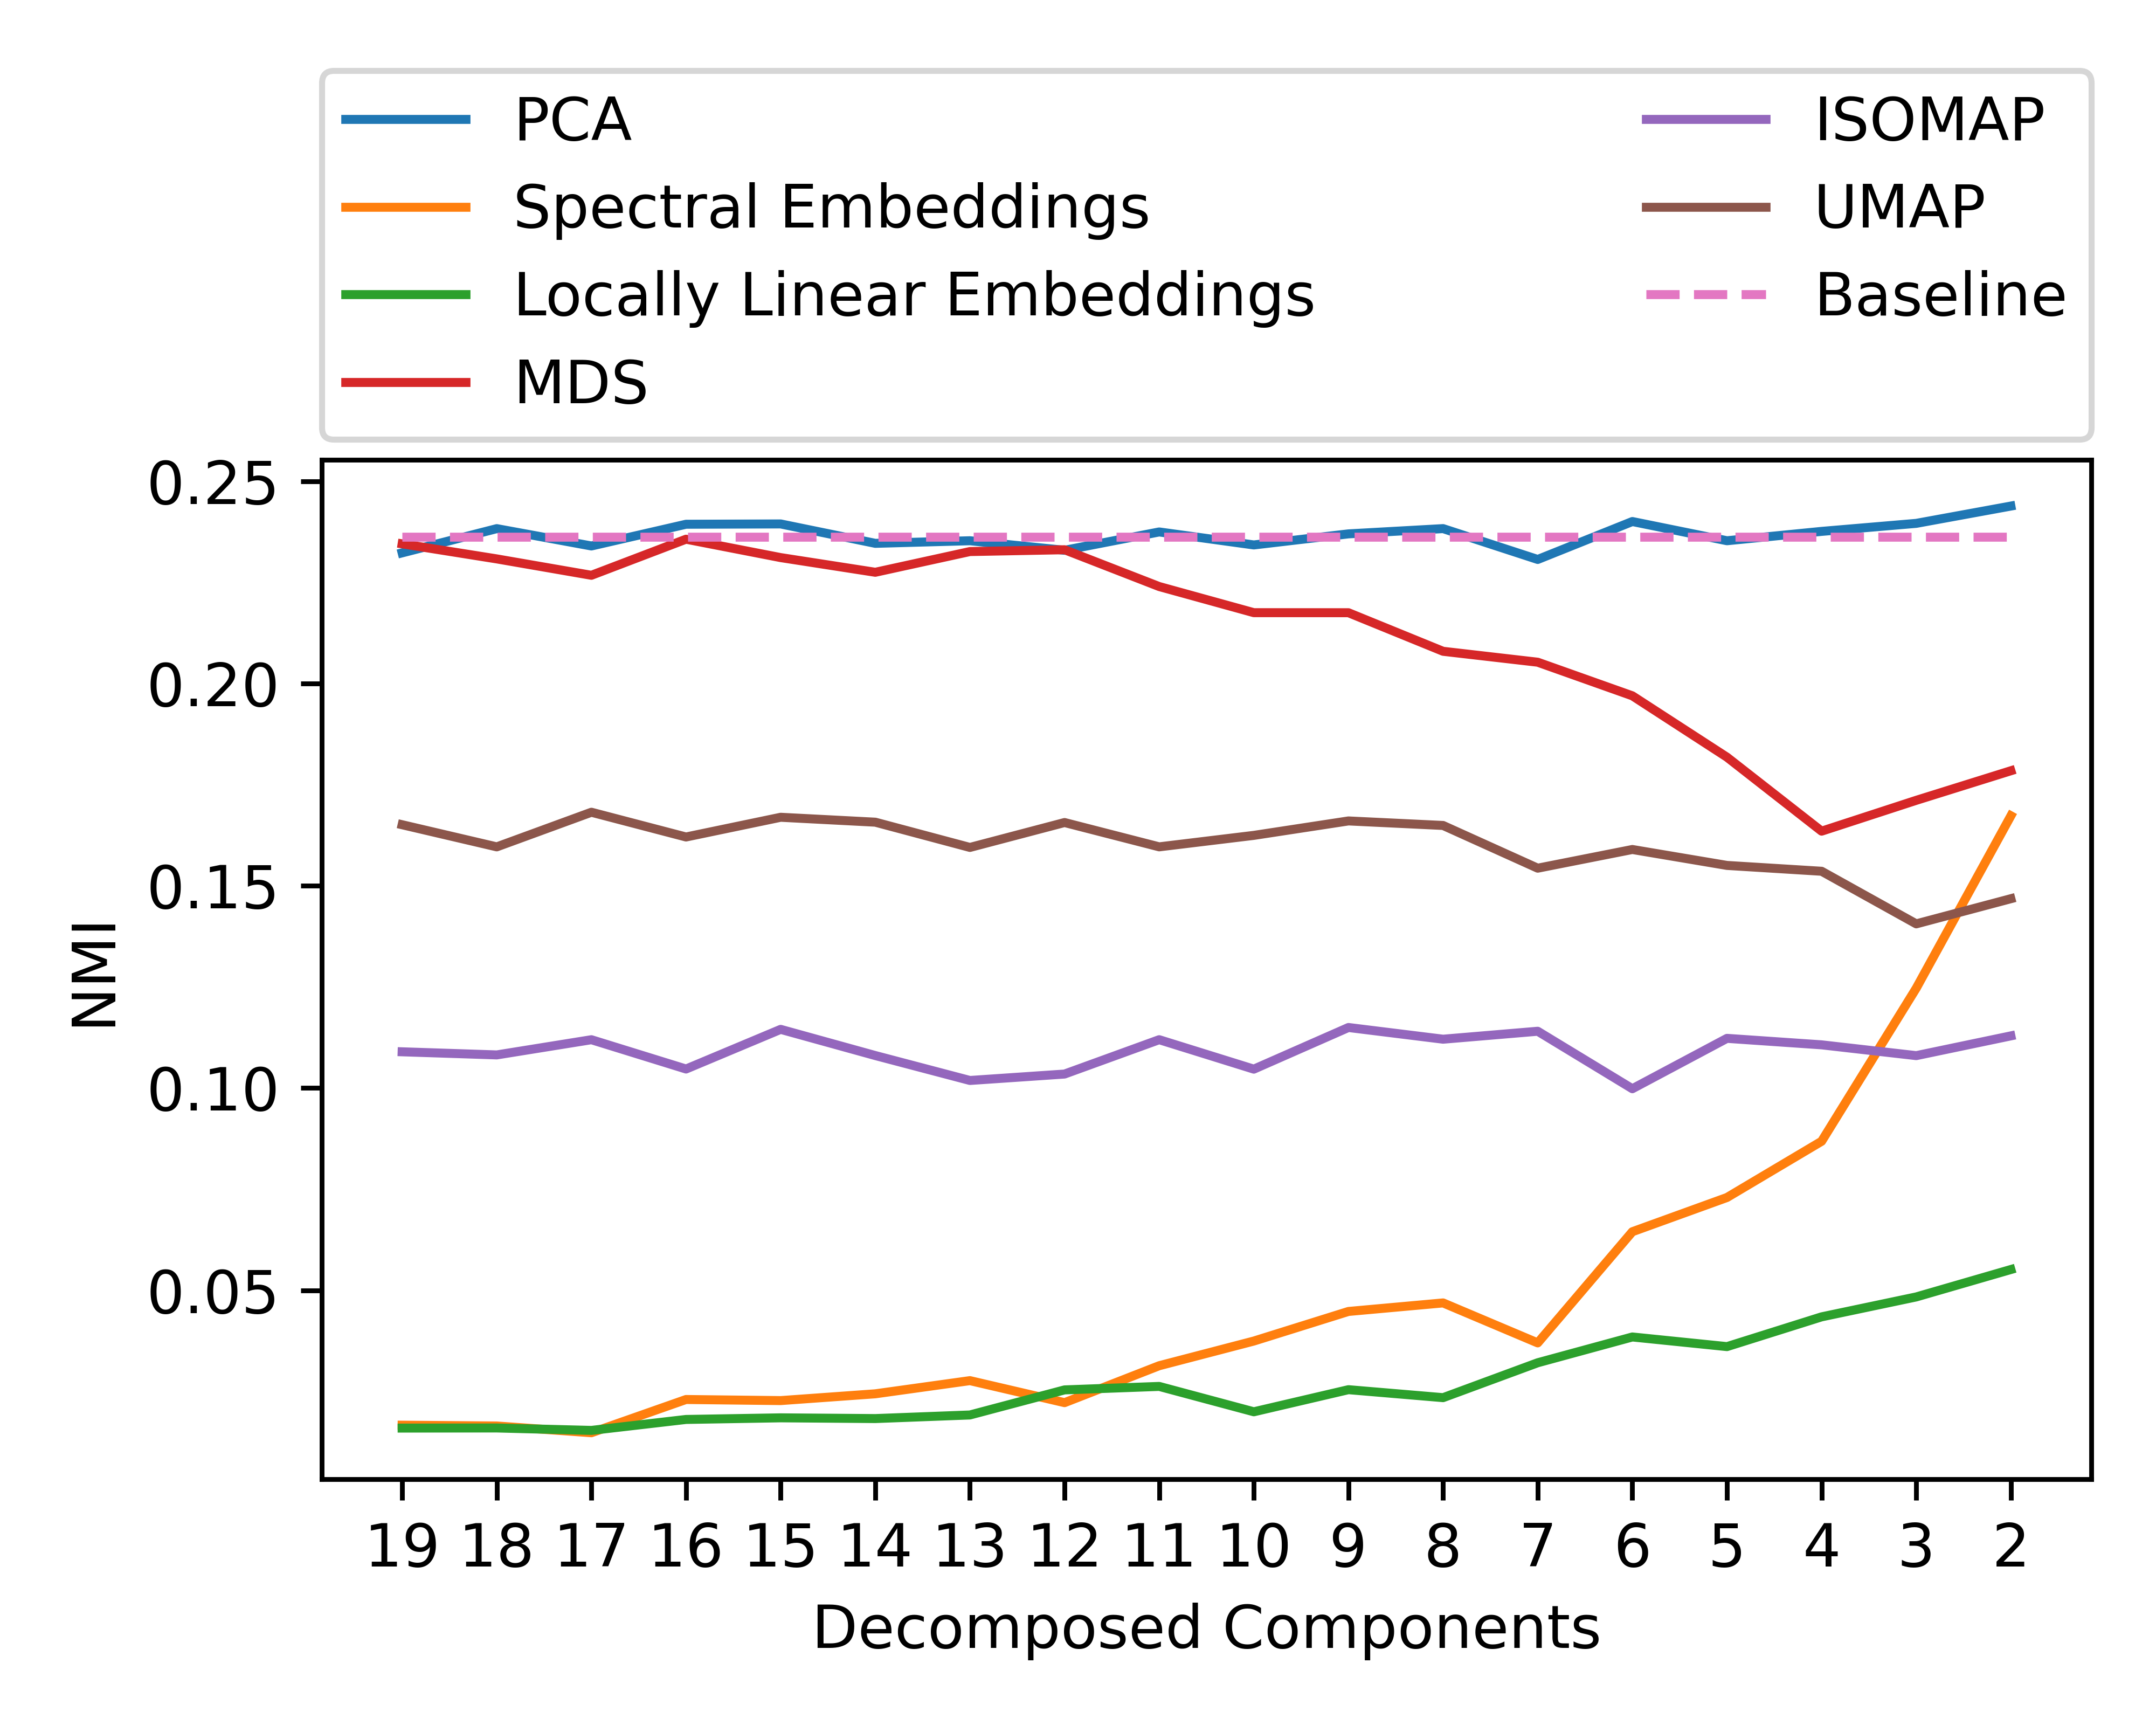
\includegraphics[width=0.48\linewidth]{images/charts/detailed_decomposition_metric_t_0.8_p_2_comparison_2_clusters_nmi.png}
                        \label{subfig:synthetic:t_0.8:dim_influence:time}
                    }
                    \caption{Анализ влияния размерности данных при различных методах снижения размерности на кластеризацию синтетического набора данных с параметром \(t = 0.8\). Результаты для
                        \subref{subfig:synthetic:t_0.8:dim_influence:ami} AMI;
                        \subref{subfig:synthetic:t_0.8:dim_influence:ari} ARI;
                        \subref{subfig:synthetic:t_0.8:dim_influence:nmi} NMI, а также на время работы алгоритма \subref{subfig:synthetic:t_influence:time}.
                    }
                    \label{fig:synthetic:t_0.8:dim_influence}
                \end{figure}

                Таким образом, эксперимент подтвердил, что даже в условиях идеальной геометрии кластеров агрессивное снижение размерности способно существенно нарушить пространственную структуру, необходимую для корректной работы \kmeans{}. Наиболее устойчивыми к снижению размерности оказались методы \hl{??????}. Это подчёркивает важность выбора метода снижения размерности в зависимости от допустимой степени искажения данных при сохранении кластерной структуры.


            \paragraph{Анализ поведения методов снижения кластеризации при сближении кластеров.}
                В данной части экспериментов особое внимание уделяется анализу устойчивости и адаптивности различных методов снижения размерности в условиях, когда кластеры в данных становятся всё менее различимыми -- то есть постепенно сближаются в пространстве признаков. Синтетическая модель, построенная как смесь нормальных распределений с контролируемым расстоянием между центрами кластеров, позволяет формализованно варьировать степень перекрытия кластеров с помощью параметра \(t\), не изменяя другие характеристики выборки.

                В условиях, когда \(t < 0\), центры кластеров максимально удаляются друг от друга без пересечений, что соответствует идеальному случаю для алгоритма \kmeans{}. По мере увеличения значения \(t\) до \(1\) центры притягиваются к общему центру масс, и границы между кластерами становятся всё менее чёткими, что моделирует реальные сценарии, в которых классы могут частично перекрываться. Такой подход позволяет объективно оценить, насколько методы понижения размерности сохраняют или теряют разделимость между группами при убывающем межкластерном расстоянии.

                Результаты экспериментов продемонстрированы на рисунке \ref{fig:synthetic:t_influence}, и показали высокую степень чувствительности к росту перекрытия кластеров.

                \hl{TBD: Analysis}

                \begin{figure}[H]\centering
                    \subfigure[]{
                        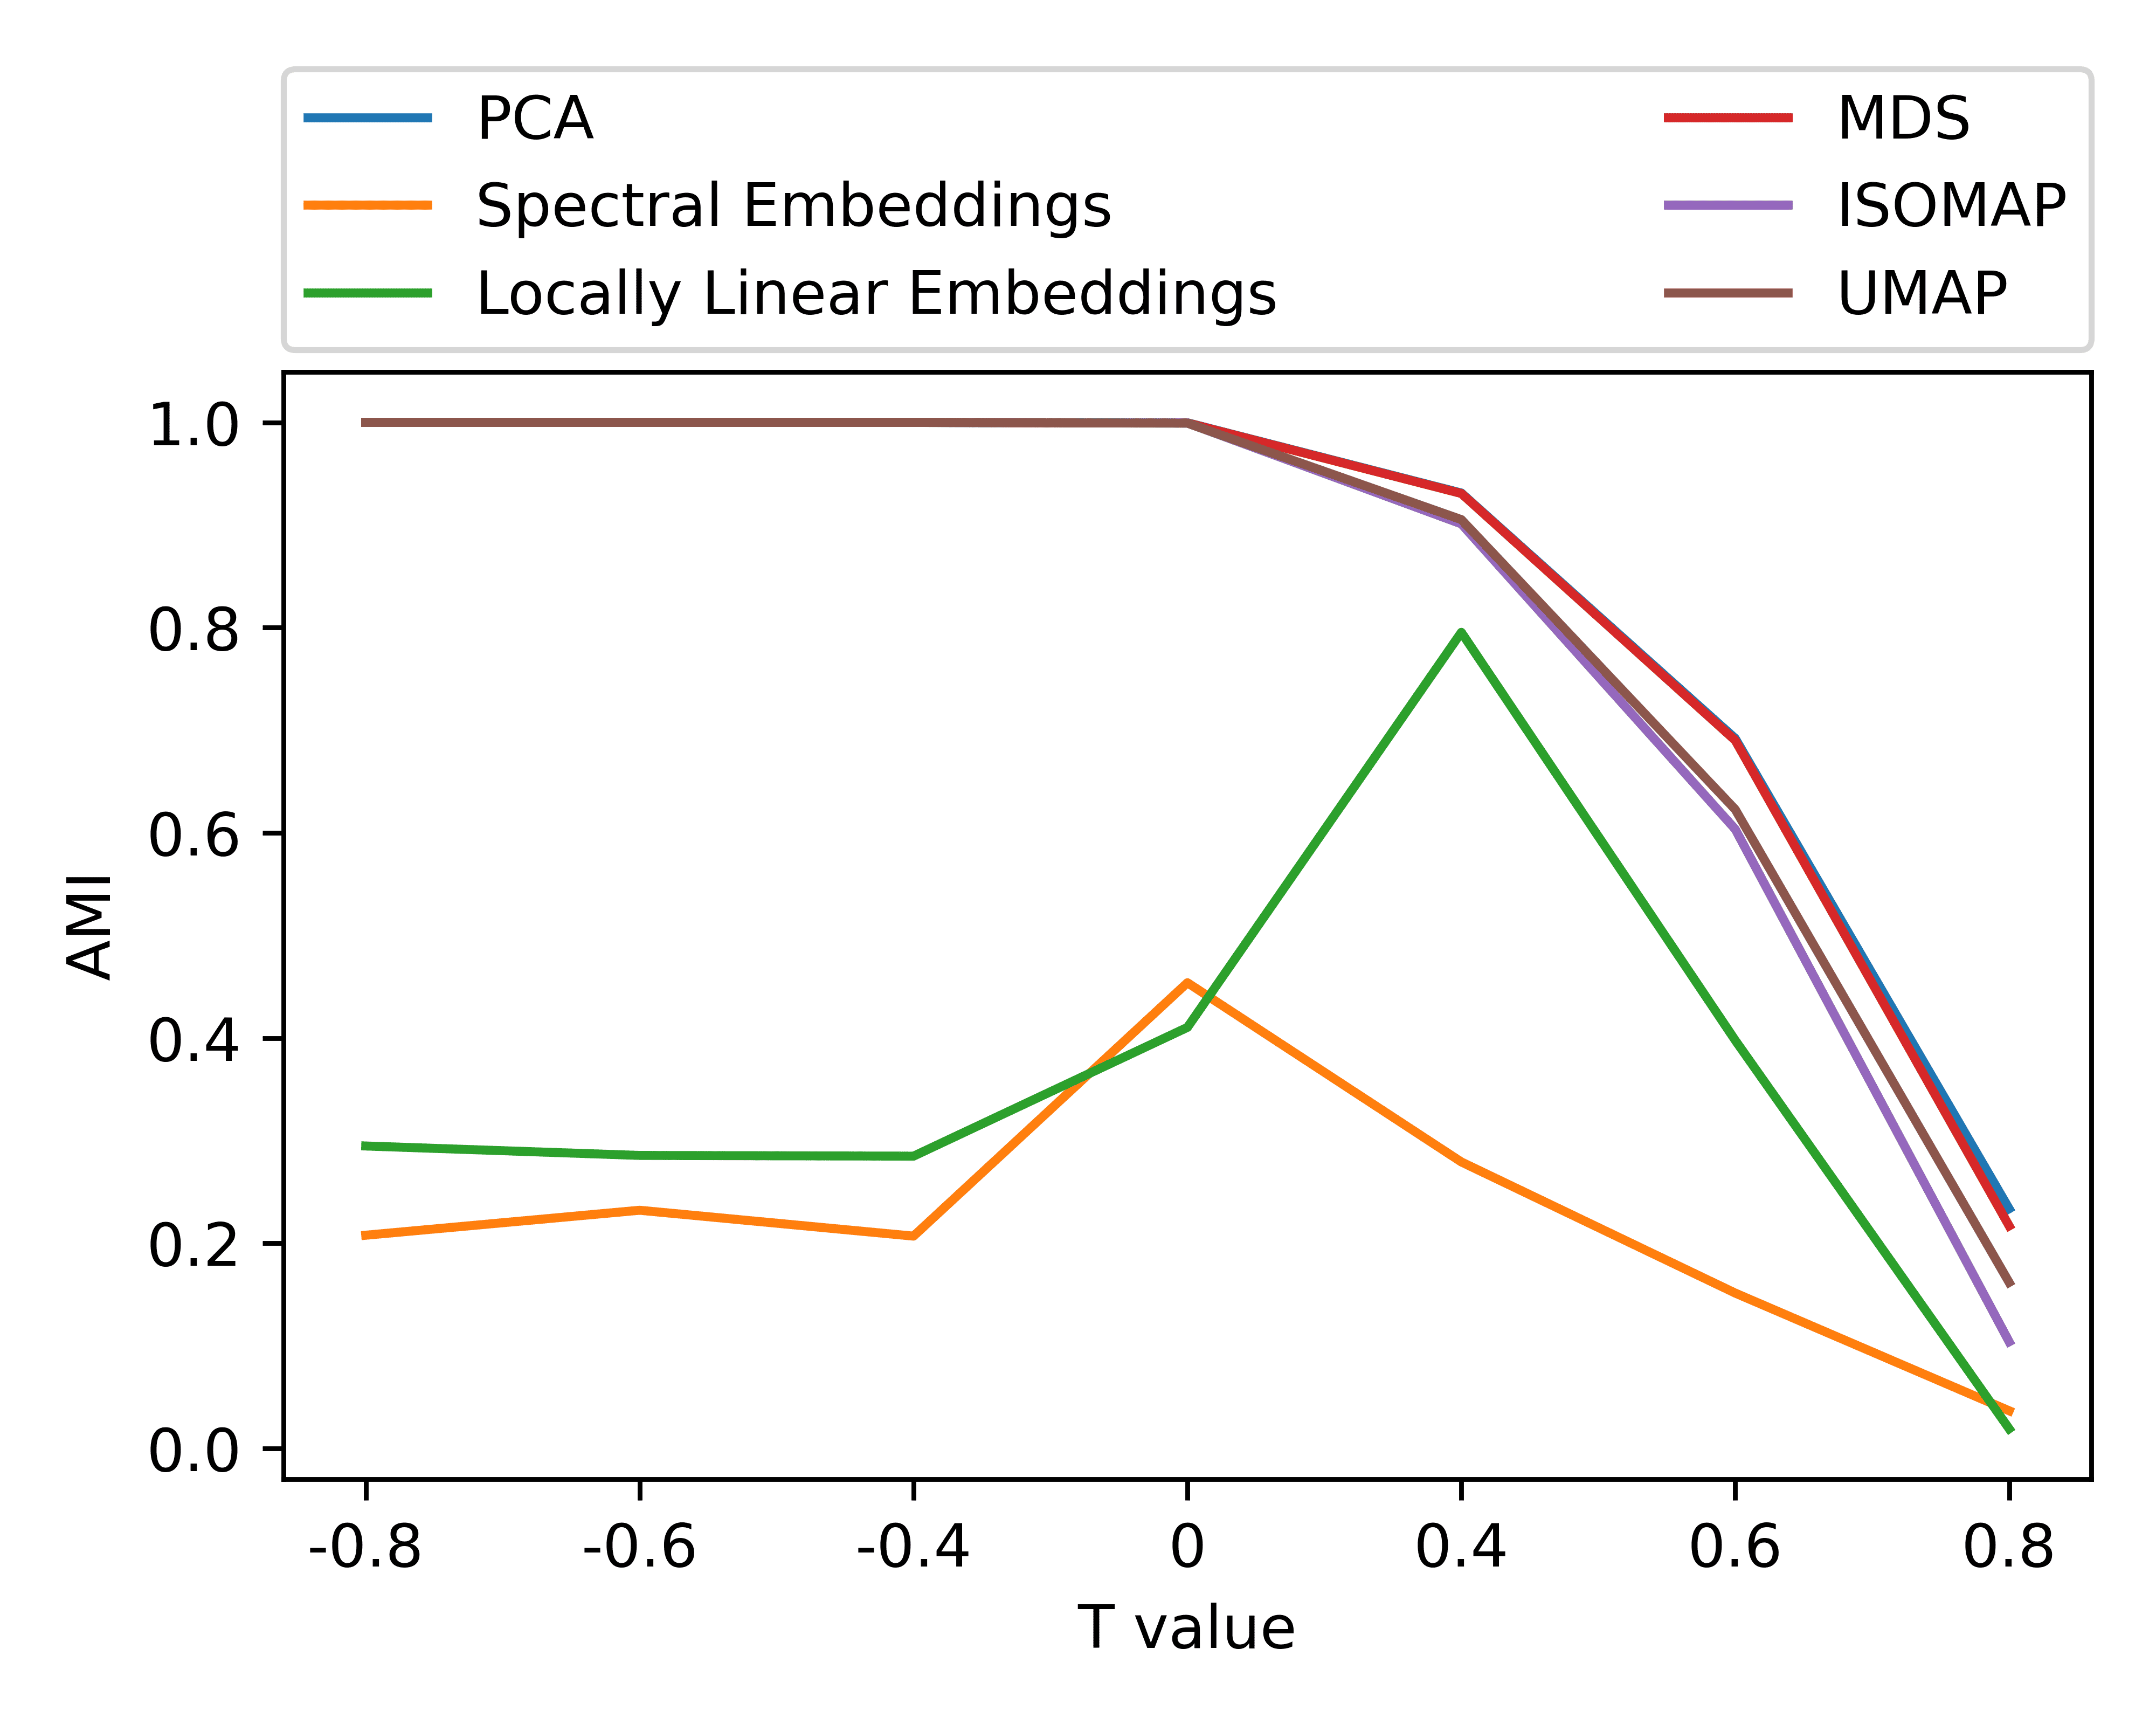
\includegraphics[width=0.48\linewidth]{images/charts/t_comparison_decomposition_20_p_2_comparison_2_clusters_ami.png}
                        \label{subfig:synthetic:t_influence:ami}
                    }
                    \subfigure[]{
                        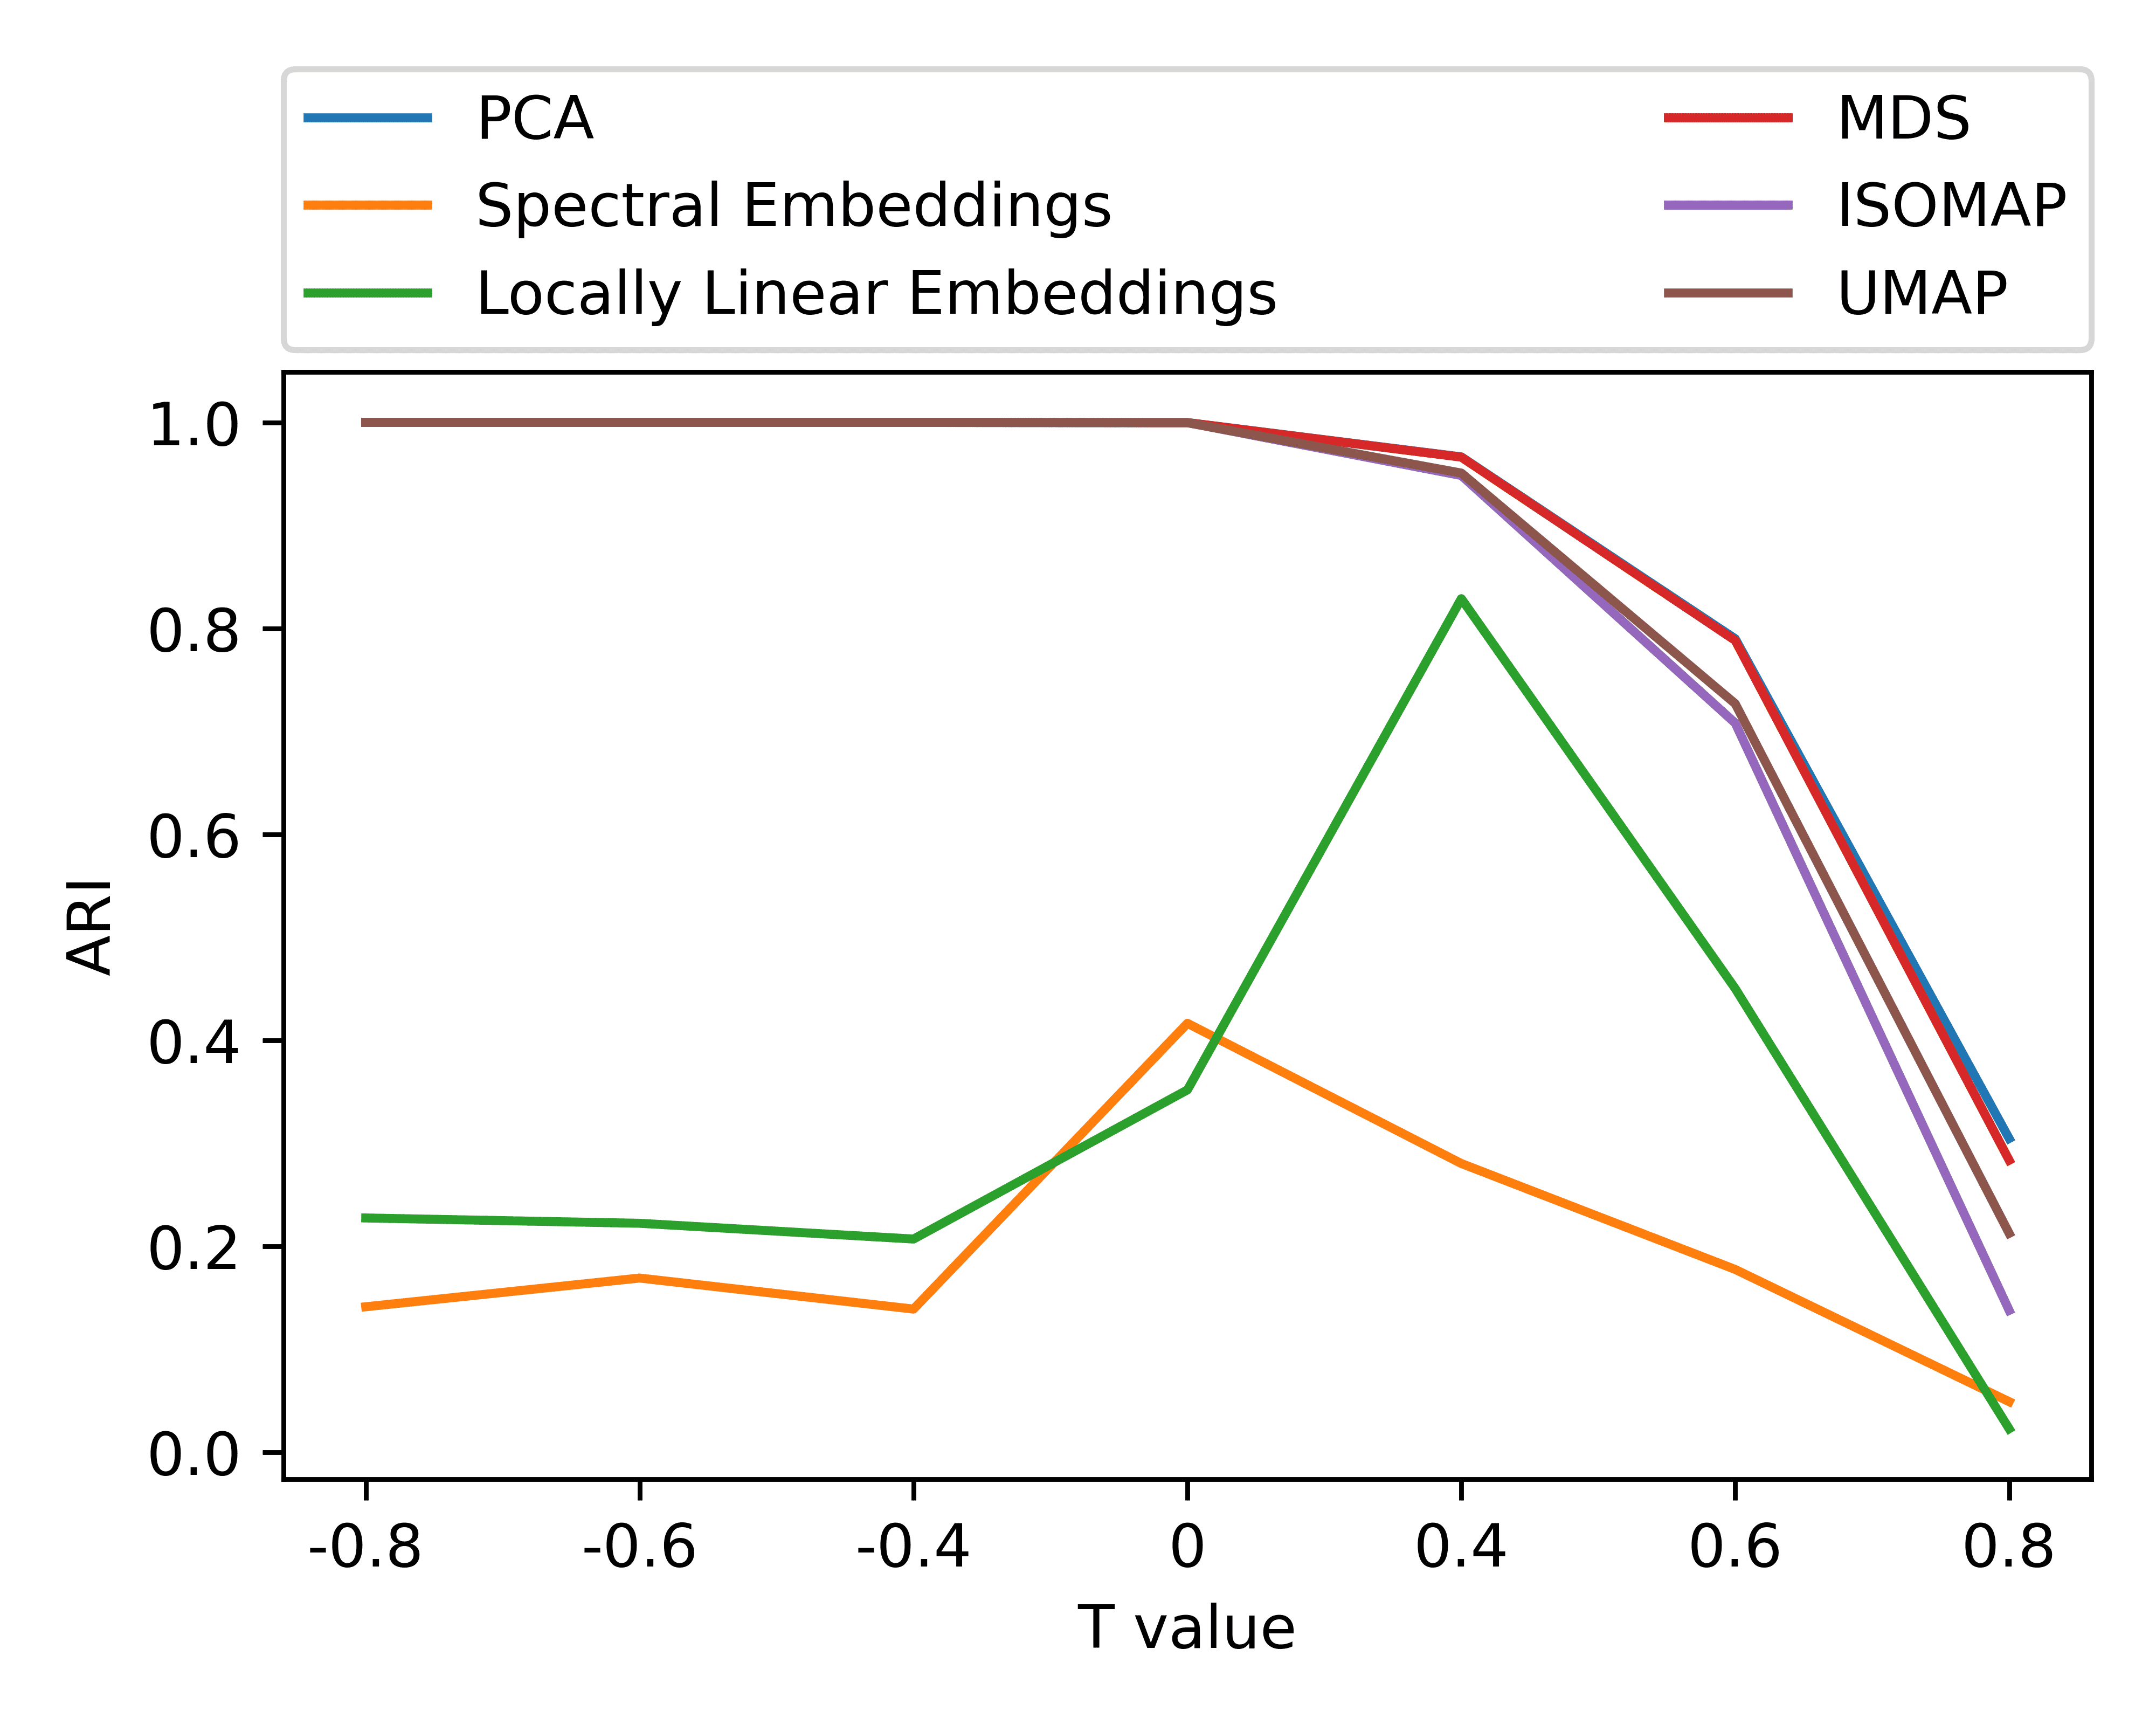
\includegraphics[width=0.48\linewidth]{images/charts/t_comparison_decomposition_20_p_2_comparison_2_clusters_ari.png}
                        \label{subfig:synthetic:t_influence:ari}
                    }
                    \subfigure[]{
                        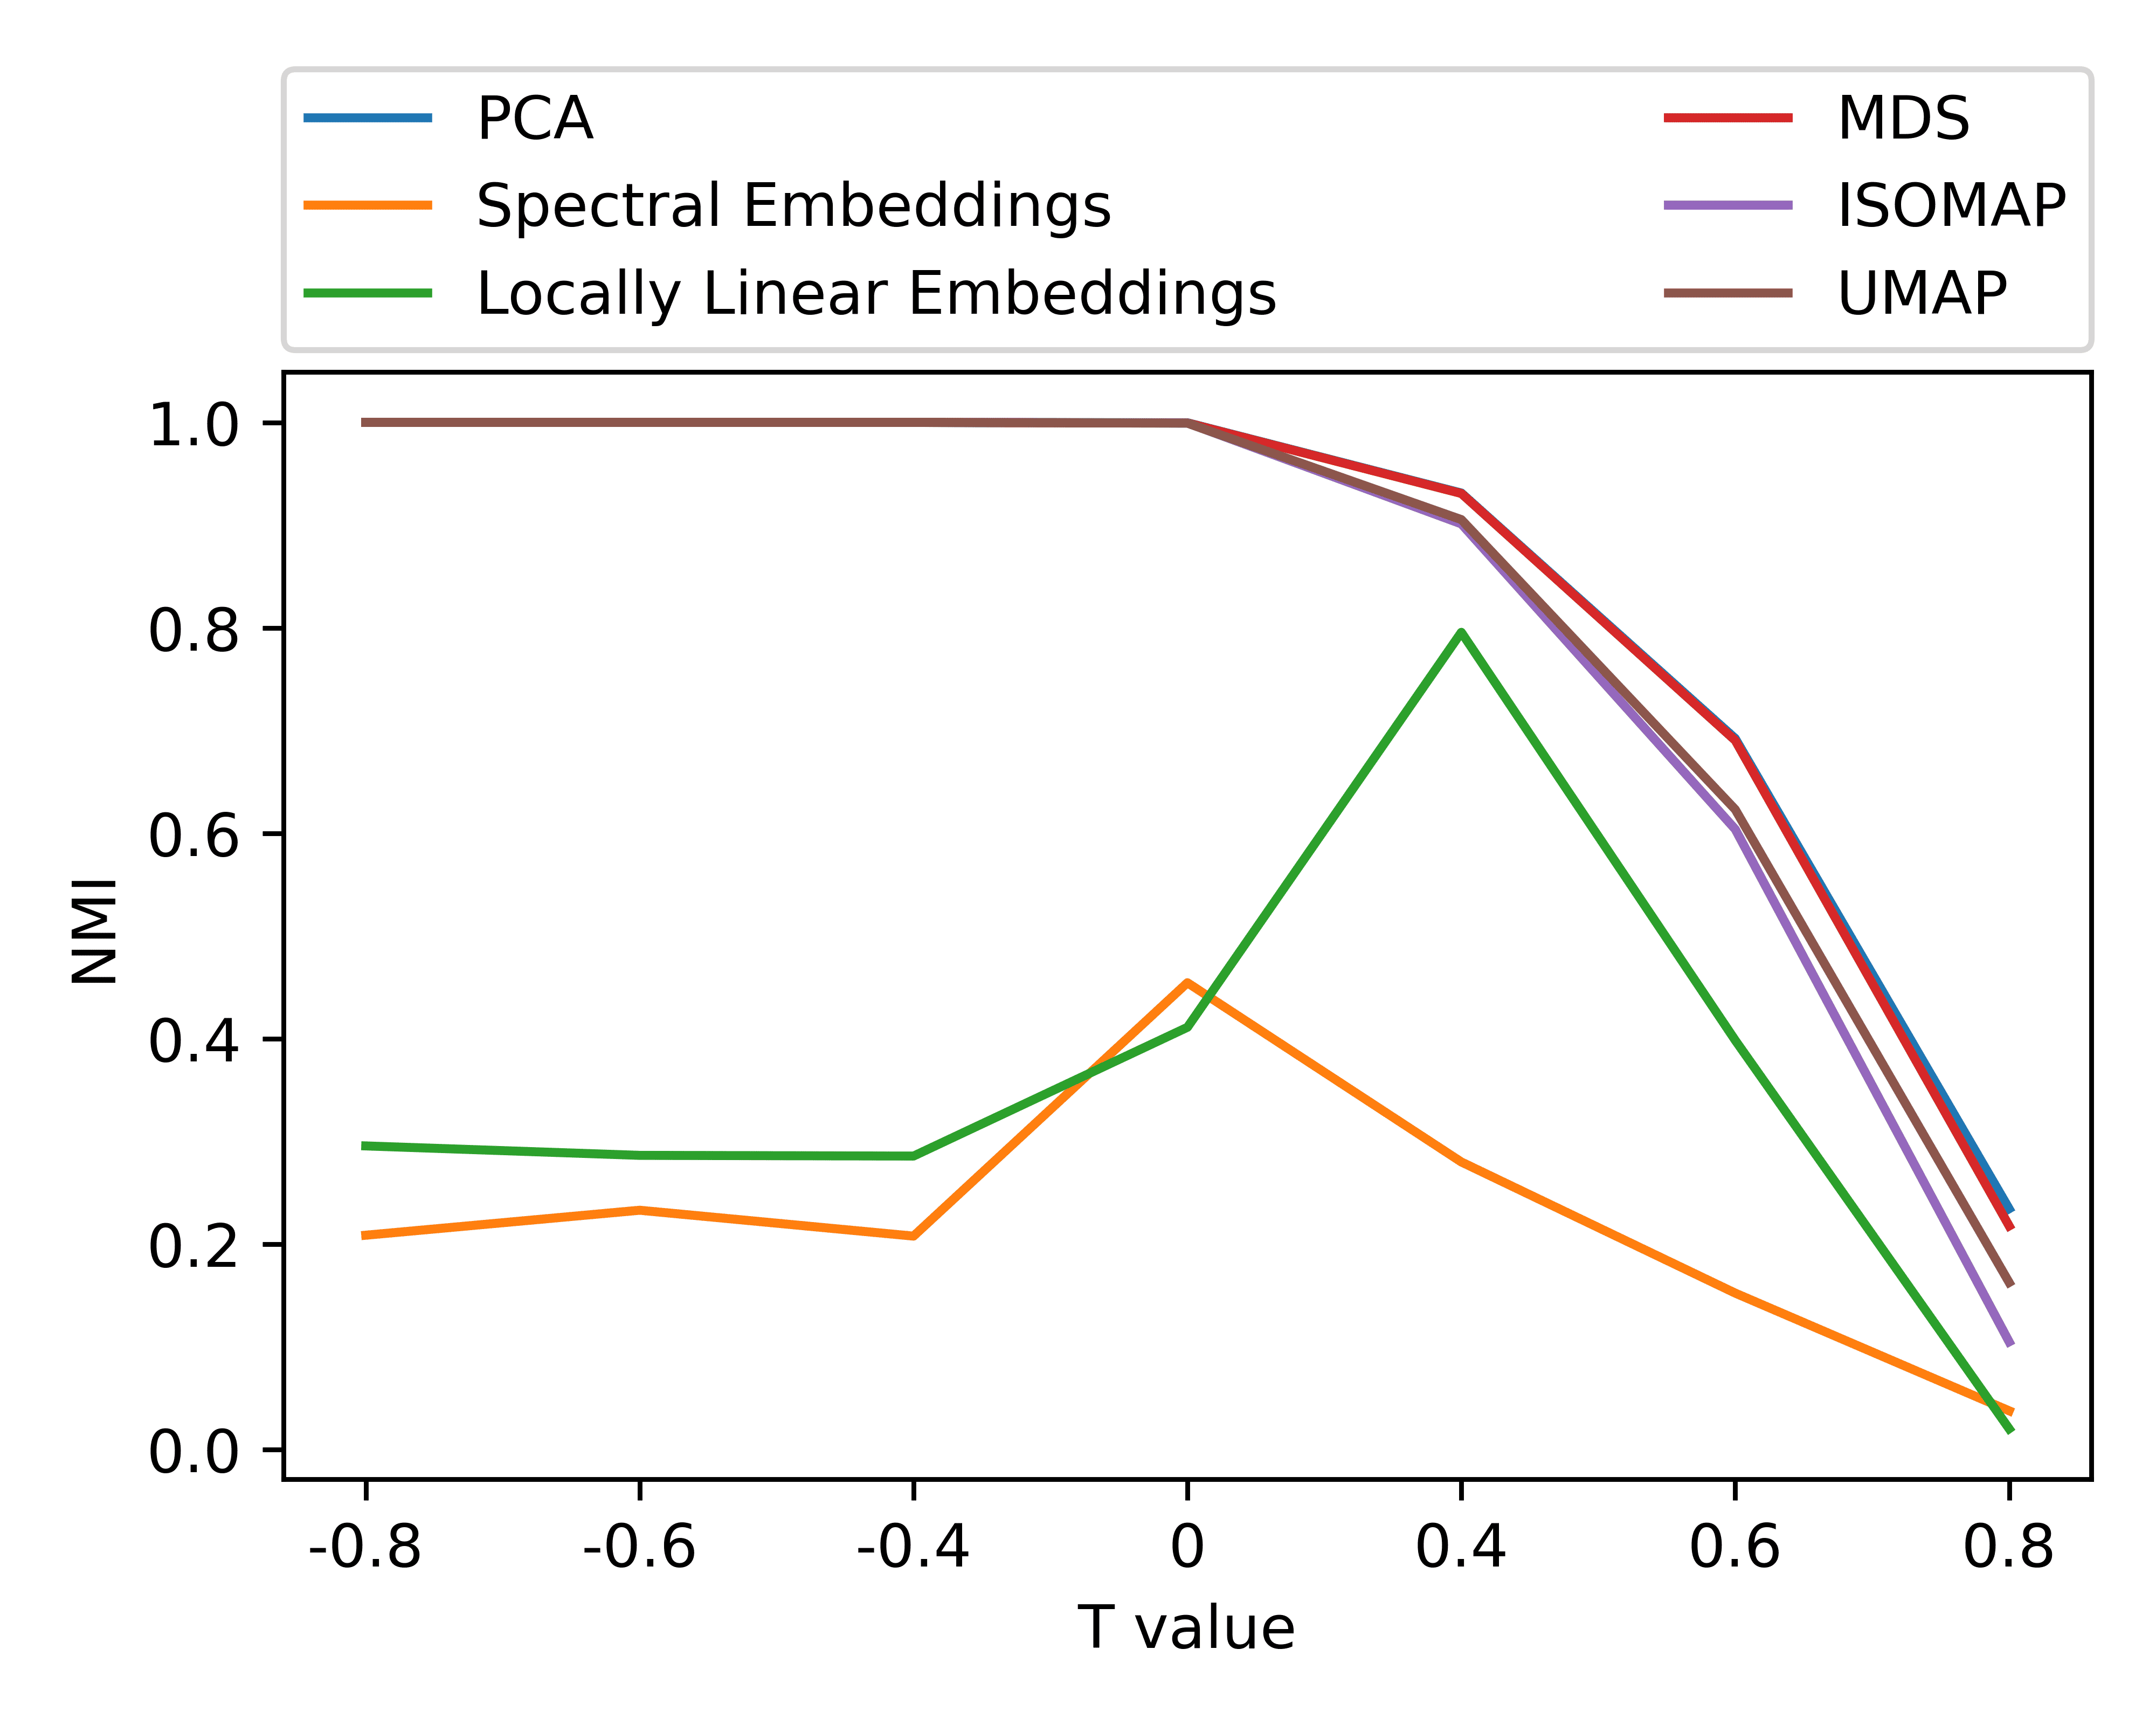
\includegraphics[width=0.48\linewidth]{images/charts/t_comparison_decomposition_20_p_2_comparison_2_clusters_nmi.png}
                        \label{subfig:synthetic:t_influence:nmi}
                    }
                    \subfigure[]{
                        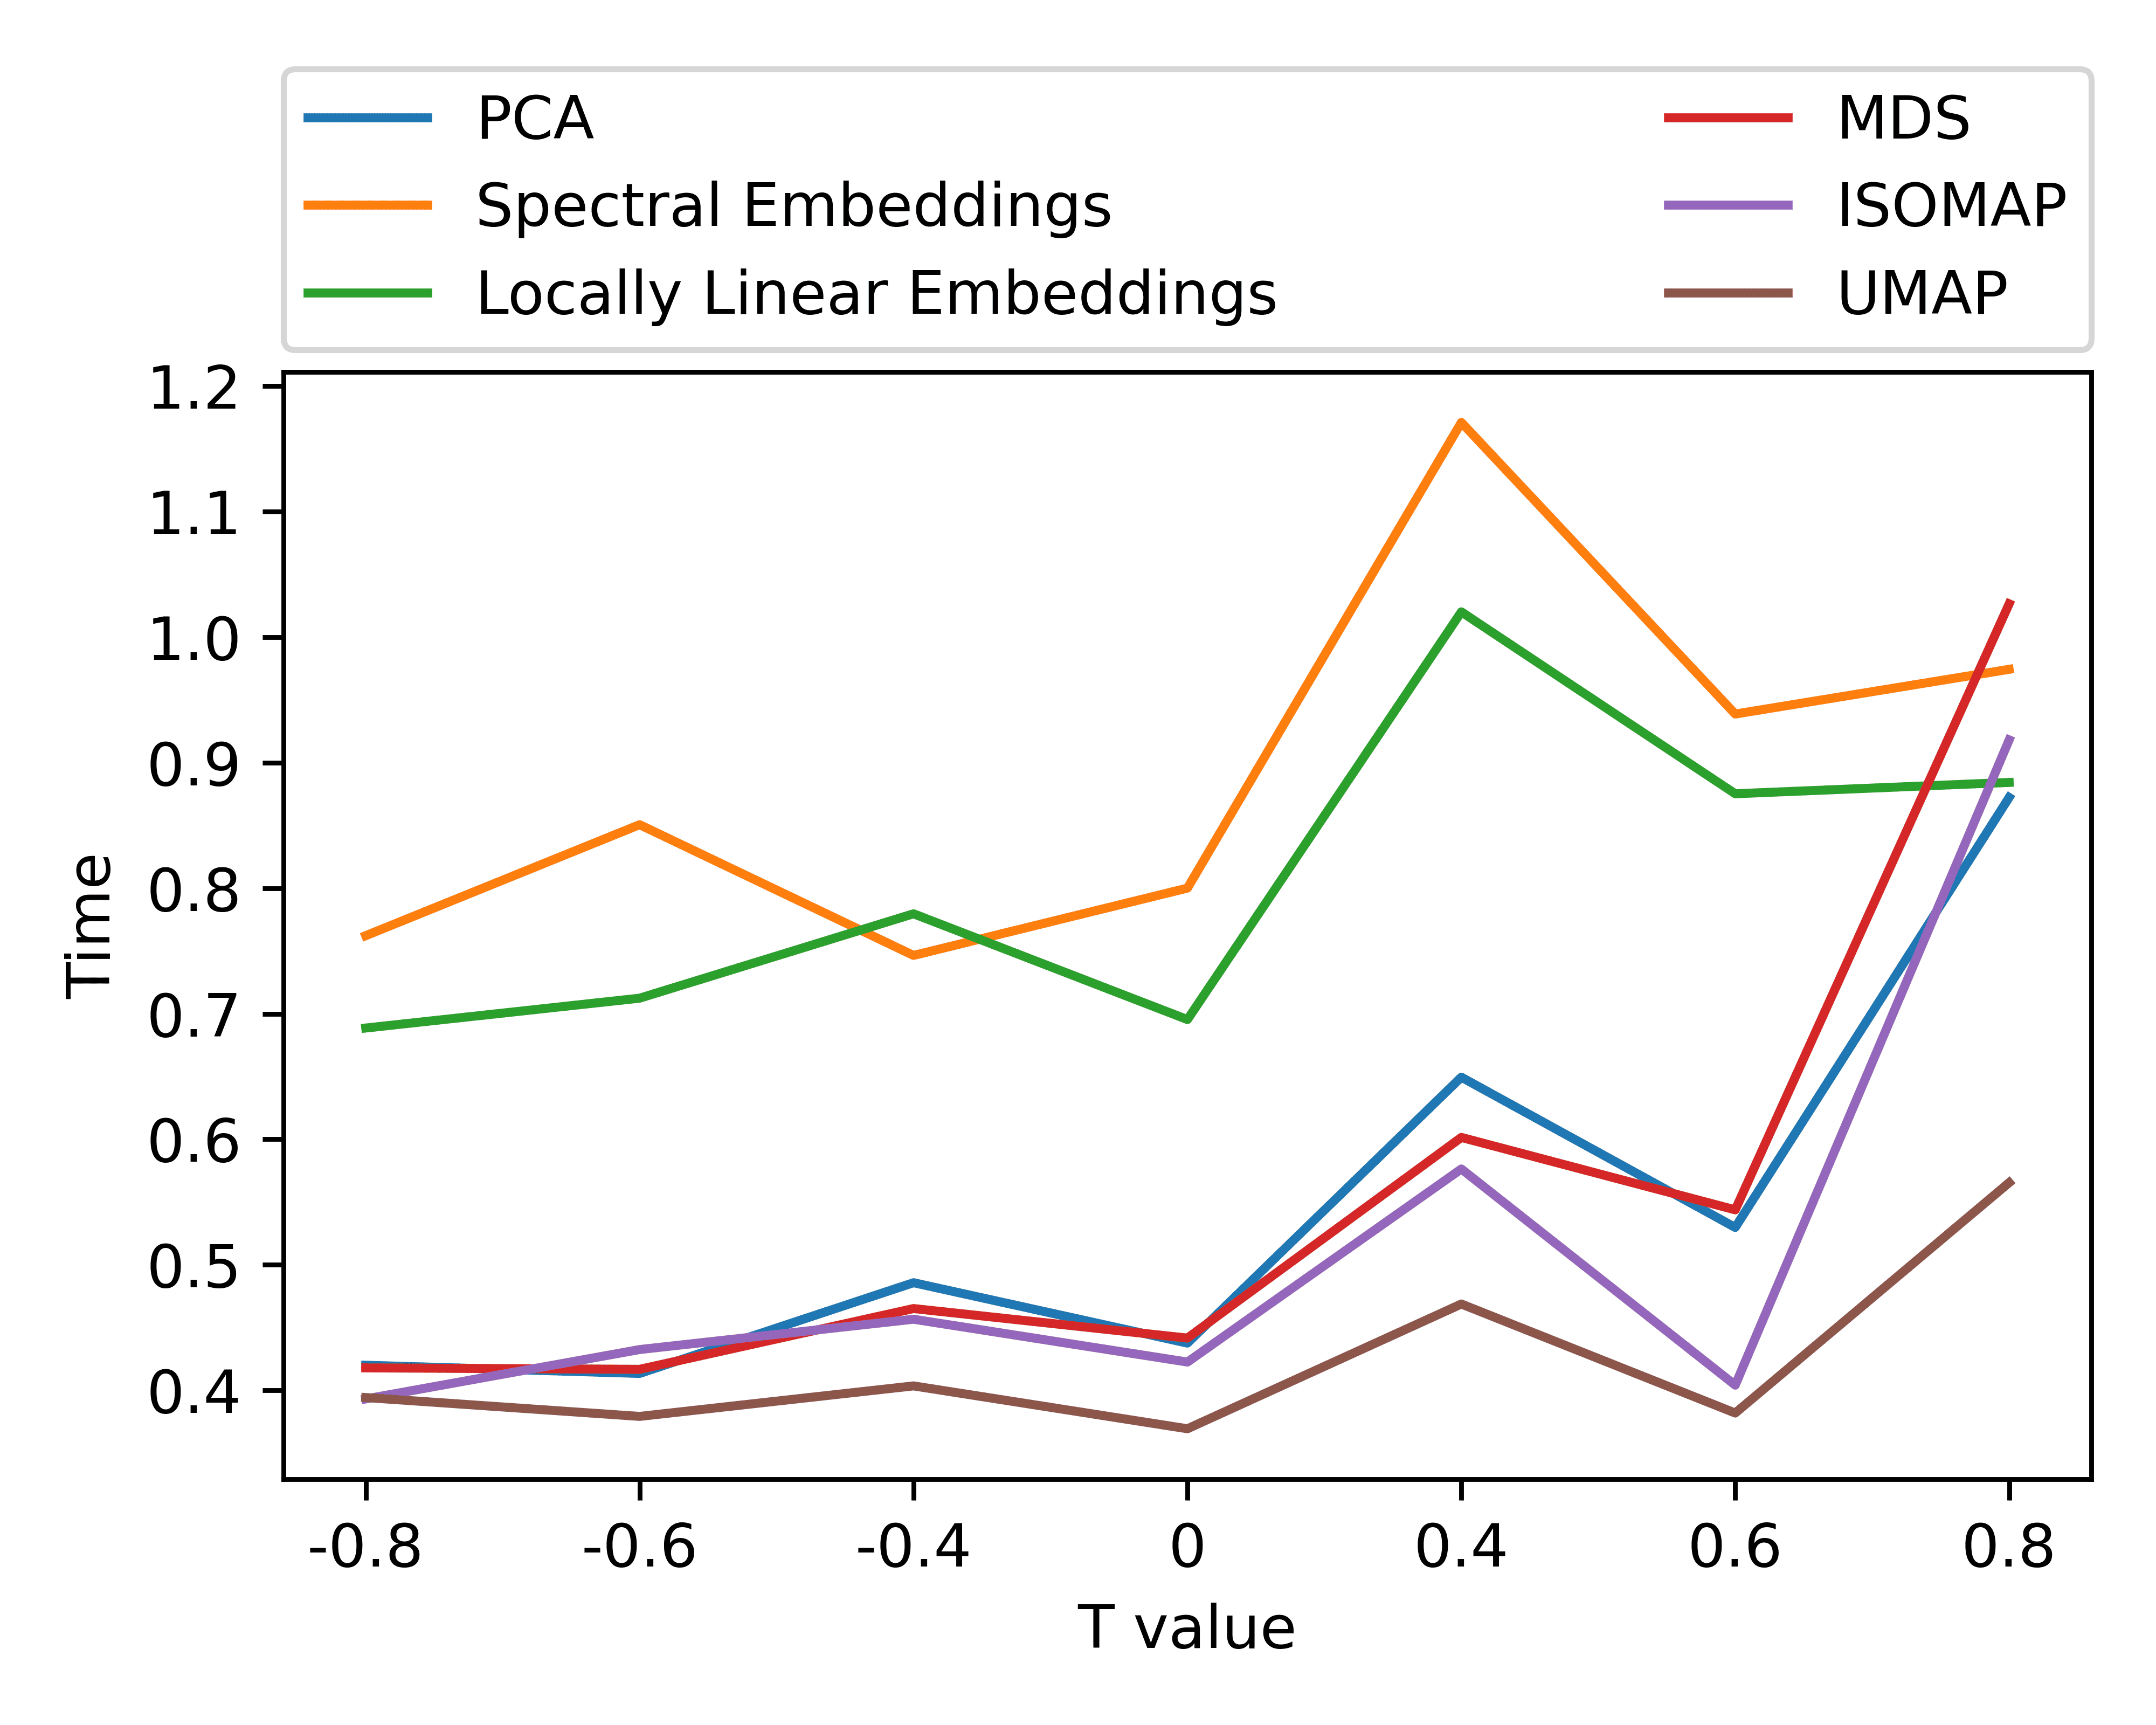
\includegraphics[width=0.48\linewidth]{images/charts/t_comparison_decomposition_20_p_2_comparison_2_clusters_time.png}
                        \label{subfig:synthetic:t_influence:time}
                    }
                    \caption{Анализ влияния различных методов снижения размерности данных на кластеризацию синтетического набора данных. Результаты для
                        \subref{subfig:synthetic:t_influence:ami} AMI;
                        \subref{subfig:synthetic:t_influence:ari} ARI;
                        \subref{subfig:synthetic:t_influence:nmi} NMI, а также на время работы алгоритма \subref{subfig:synthetic:t_influence:time}.
                    }
                    \label{fig:synthetic:t_influence}
                \end{figure}

                Таким образом, анализ на синтетических данных подтвердил, что эффективность методов снижения размерности сильно зависит от геометрии и плотности кластеров. Это подчёркивает необходимость адаптивного выбора метода снижения размерности в зависимости от ожидаемой сложности кластерной структуры в данных.

        \subsubsection{Эксперименты на реальных данных}
            Также предложенный подход был исследован на реальных данных. Для этого было решено использовать несколько стандартных наборов данных:

            \begin{itemize}
                \item Breast Cancer,
                \item Digits,
                \item Wine.
            \end{itemize}

            \paragraph{Результаты алгоритма на наборе данных Breast Cancer.}
                Breast Cancer — это стандартный набор данных для бинарной классификации, часто используемый в задачах медицинской диагностики. Данные содержат результаты измерений опухолей молочной железы, полученные при помощи тонкоигольной аспирационной биопсии (FNA). Каждая запись включает характеристики клеточных ядер, такие как радиус, текстура, периметр и другие морфологические признаки.

                \begin{table}[H]
                    \centering
                    \caption{Характеристики набора данных Breast Cancer.}
                    \begin{tabular}{ccc}
                        \toprule
                        Число классов & Число объектов & Размерность пространства \\
                        \midrule
                        2 & 569 & 30 \\
                        \bottomrule
                    \end{tabular}
                \end{table}

                Набор данных Breast Cancer представляет собой матрицу размерностью 569x30, где каждая строка соответствует отдельному образцу опухоли, а каждый столбец содержит числовое значение одного из диагностических признаков. Целевая переменная указывает на доброкачественность (benign) или злокачественность (malignant) новообразования. Данные часто используются для обучения моделей машинного обучения, направленных на автоматизацию диагностики рака молочной железы.

                \begin{figure}[H]\centering
                    \subfigure[]{
                        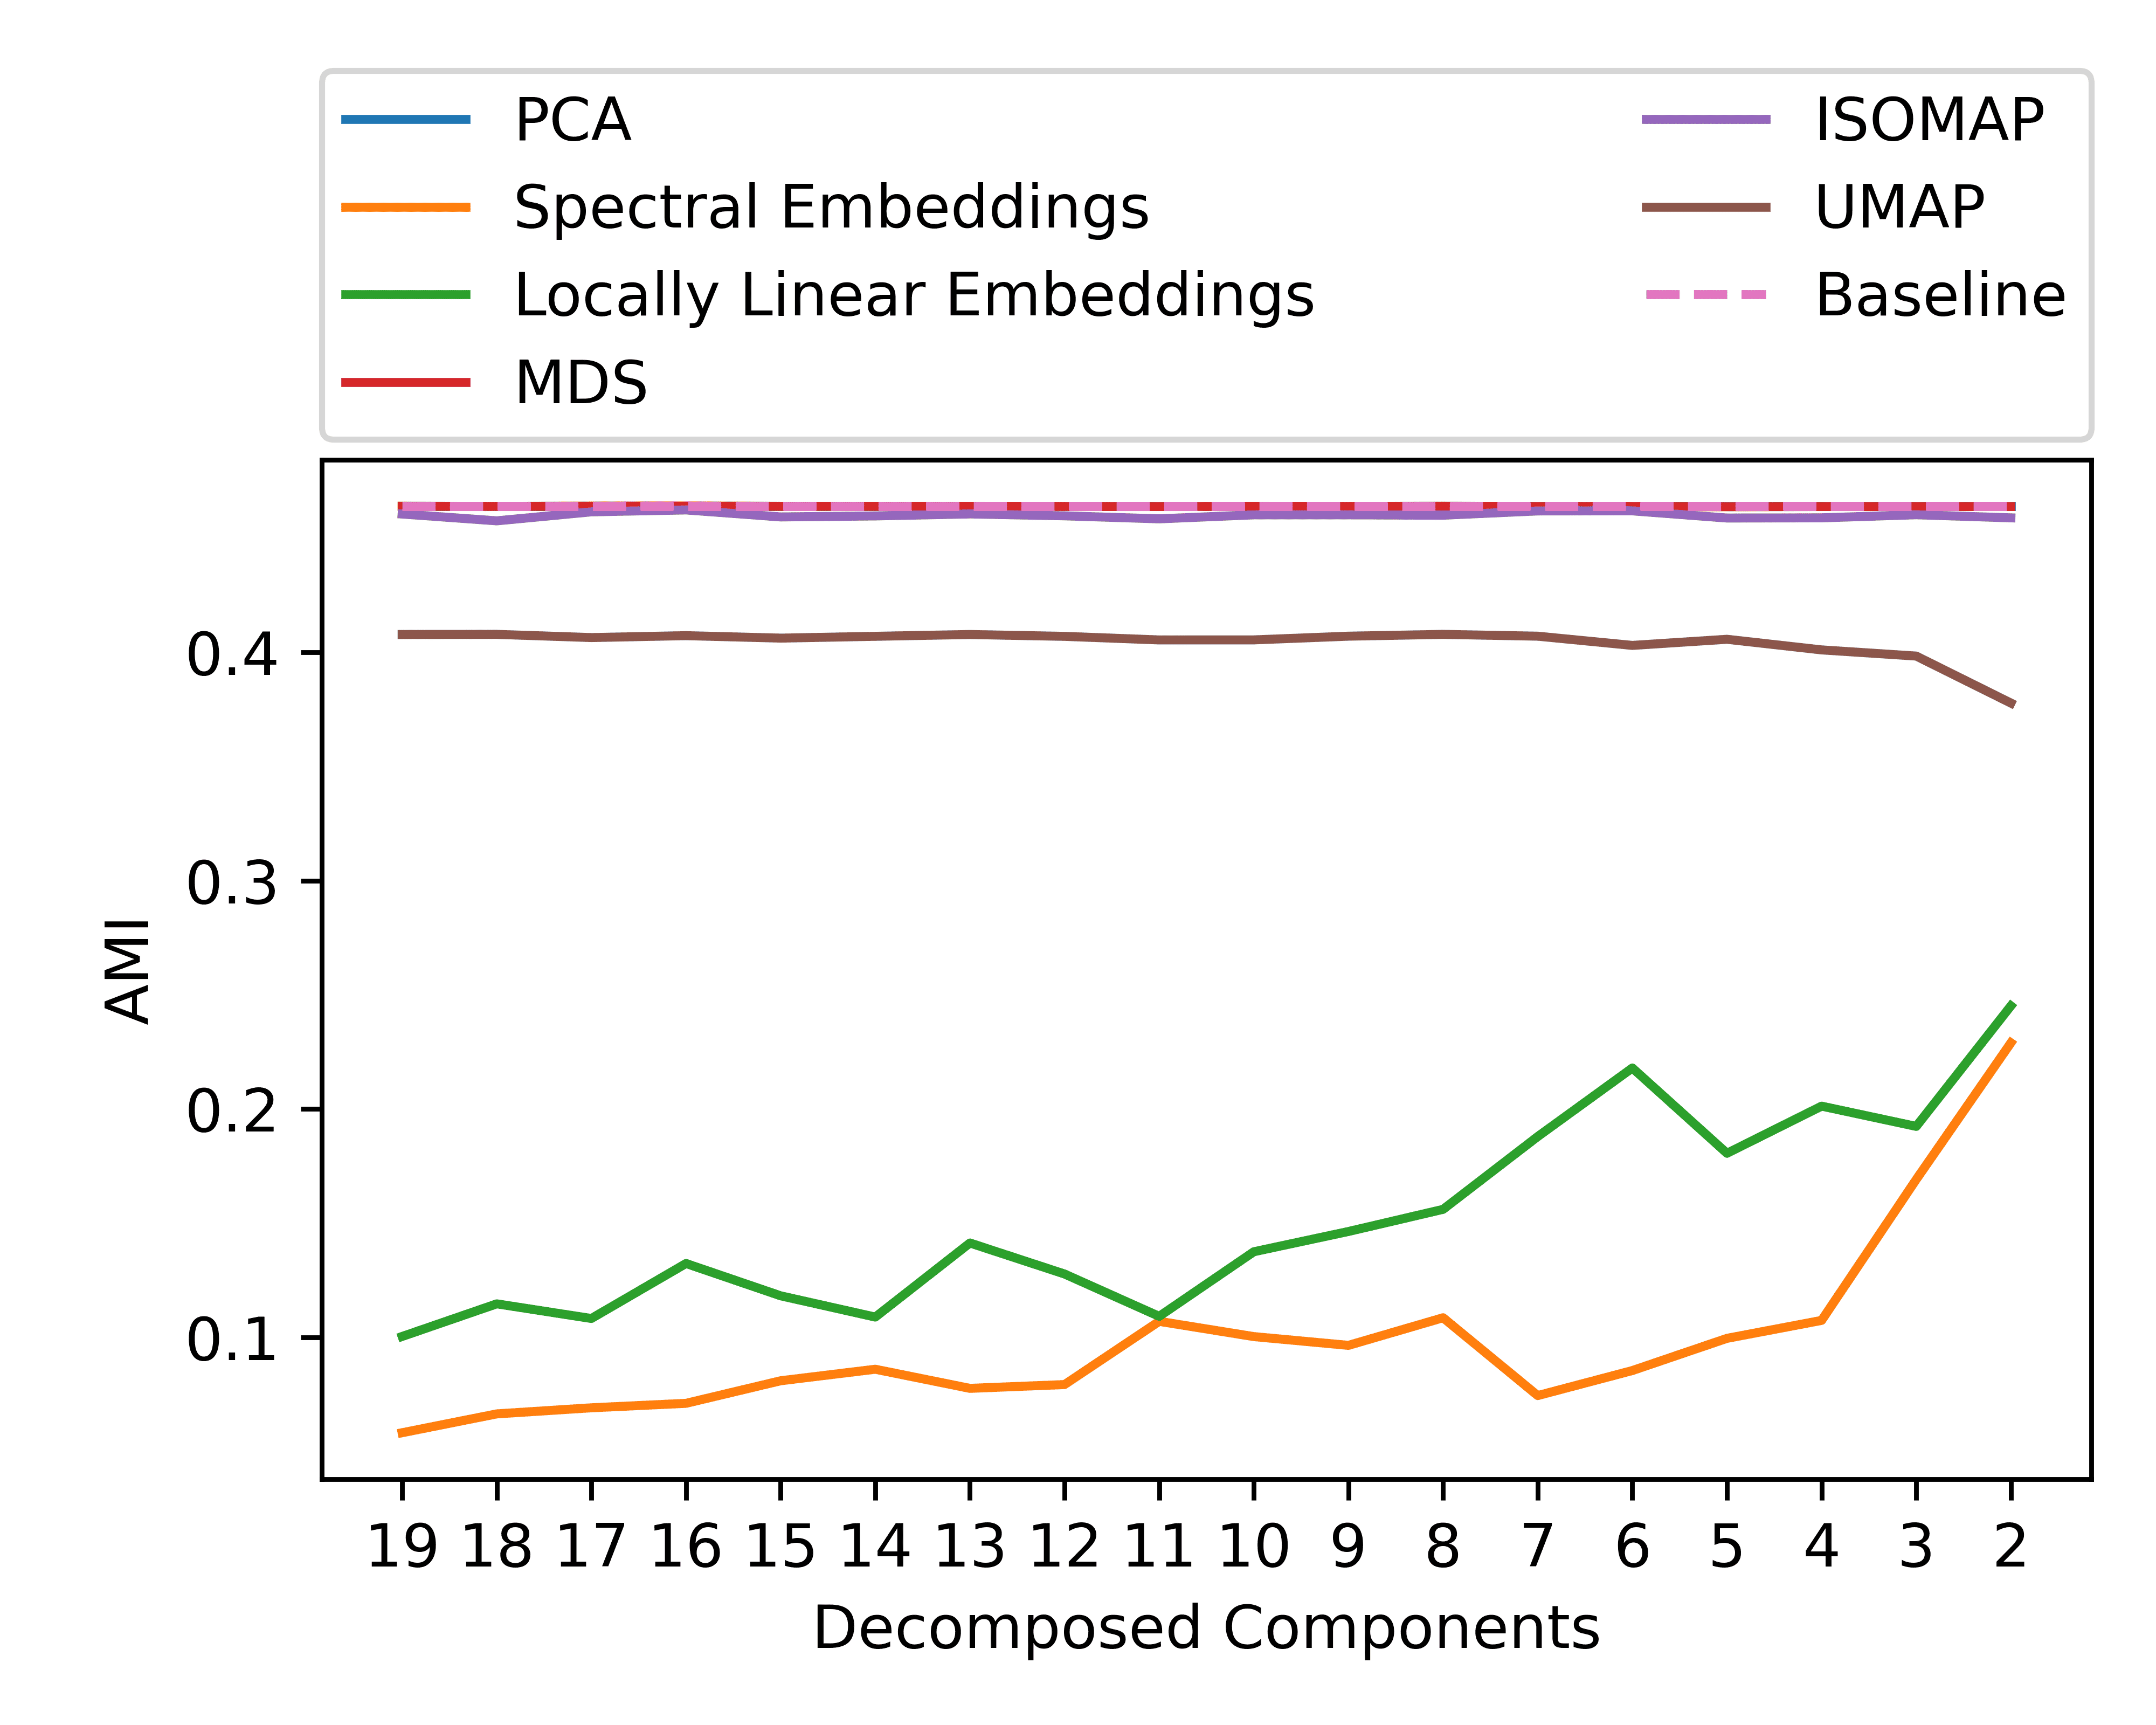
\includegraphics[width=0.48\linewidth]{images/charts_real/real_data_breast_cancer_ami.png}
                        \label{subfig:breast_cancer:ami}
                    }
                    \subfigure[]{
                        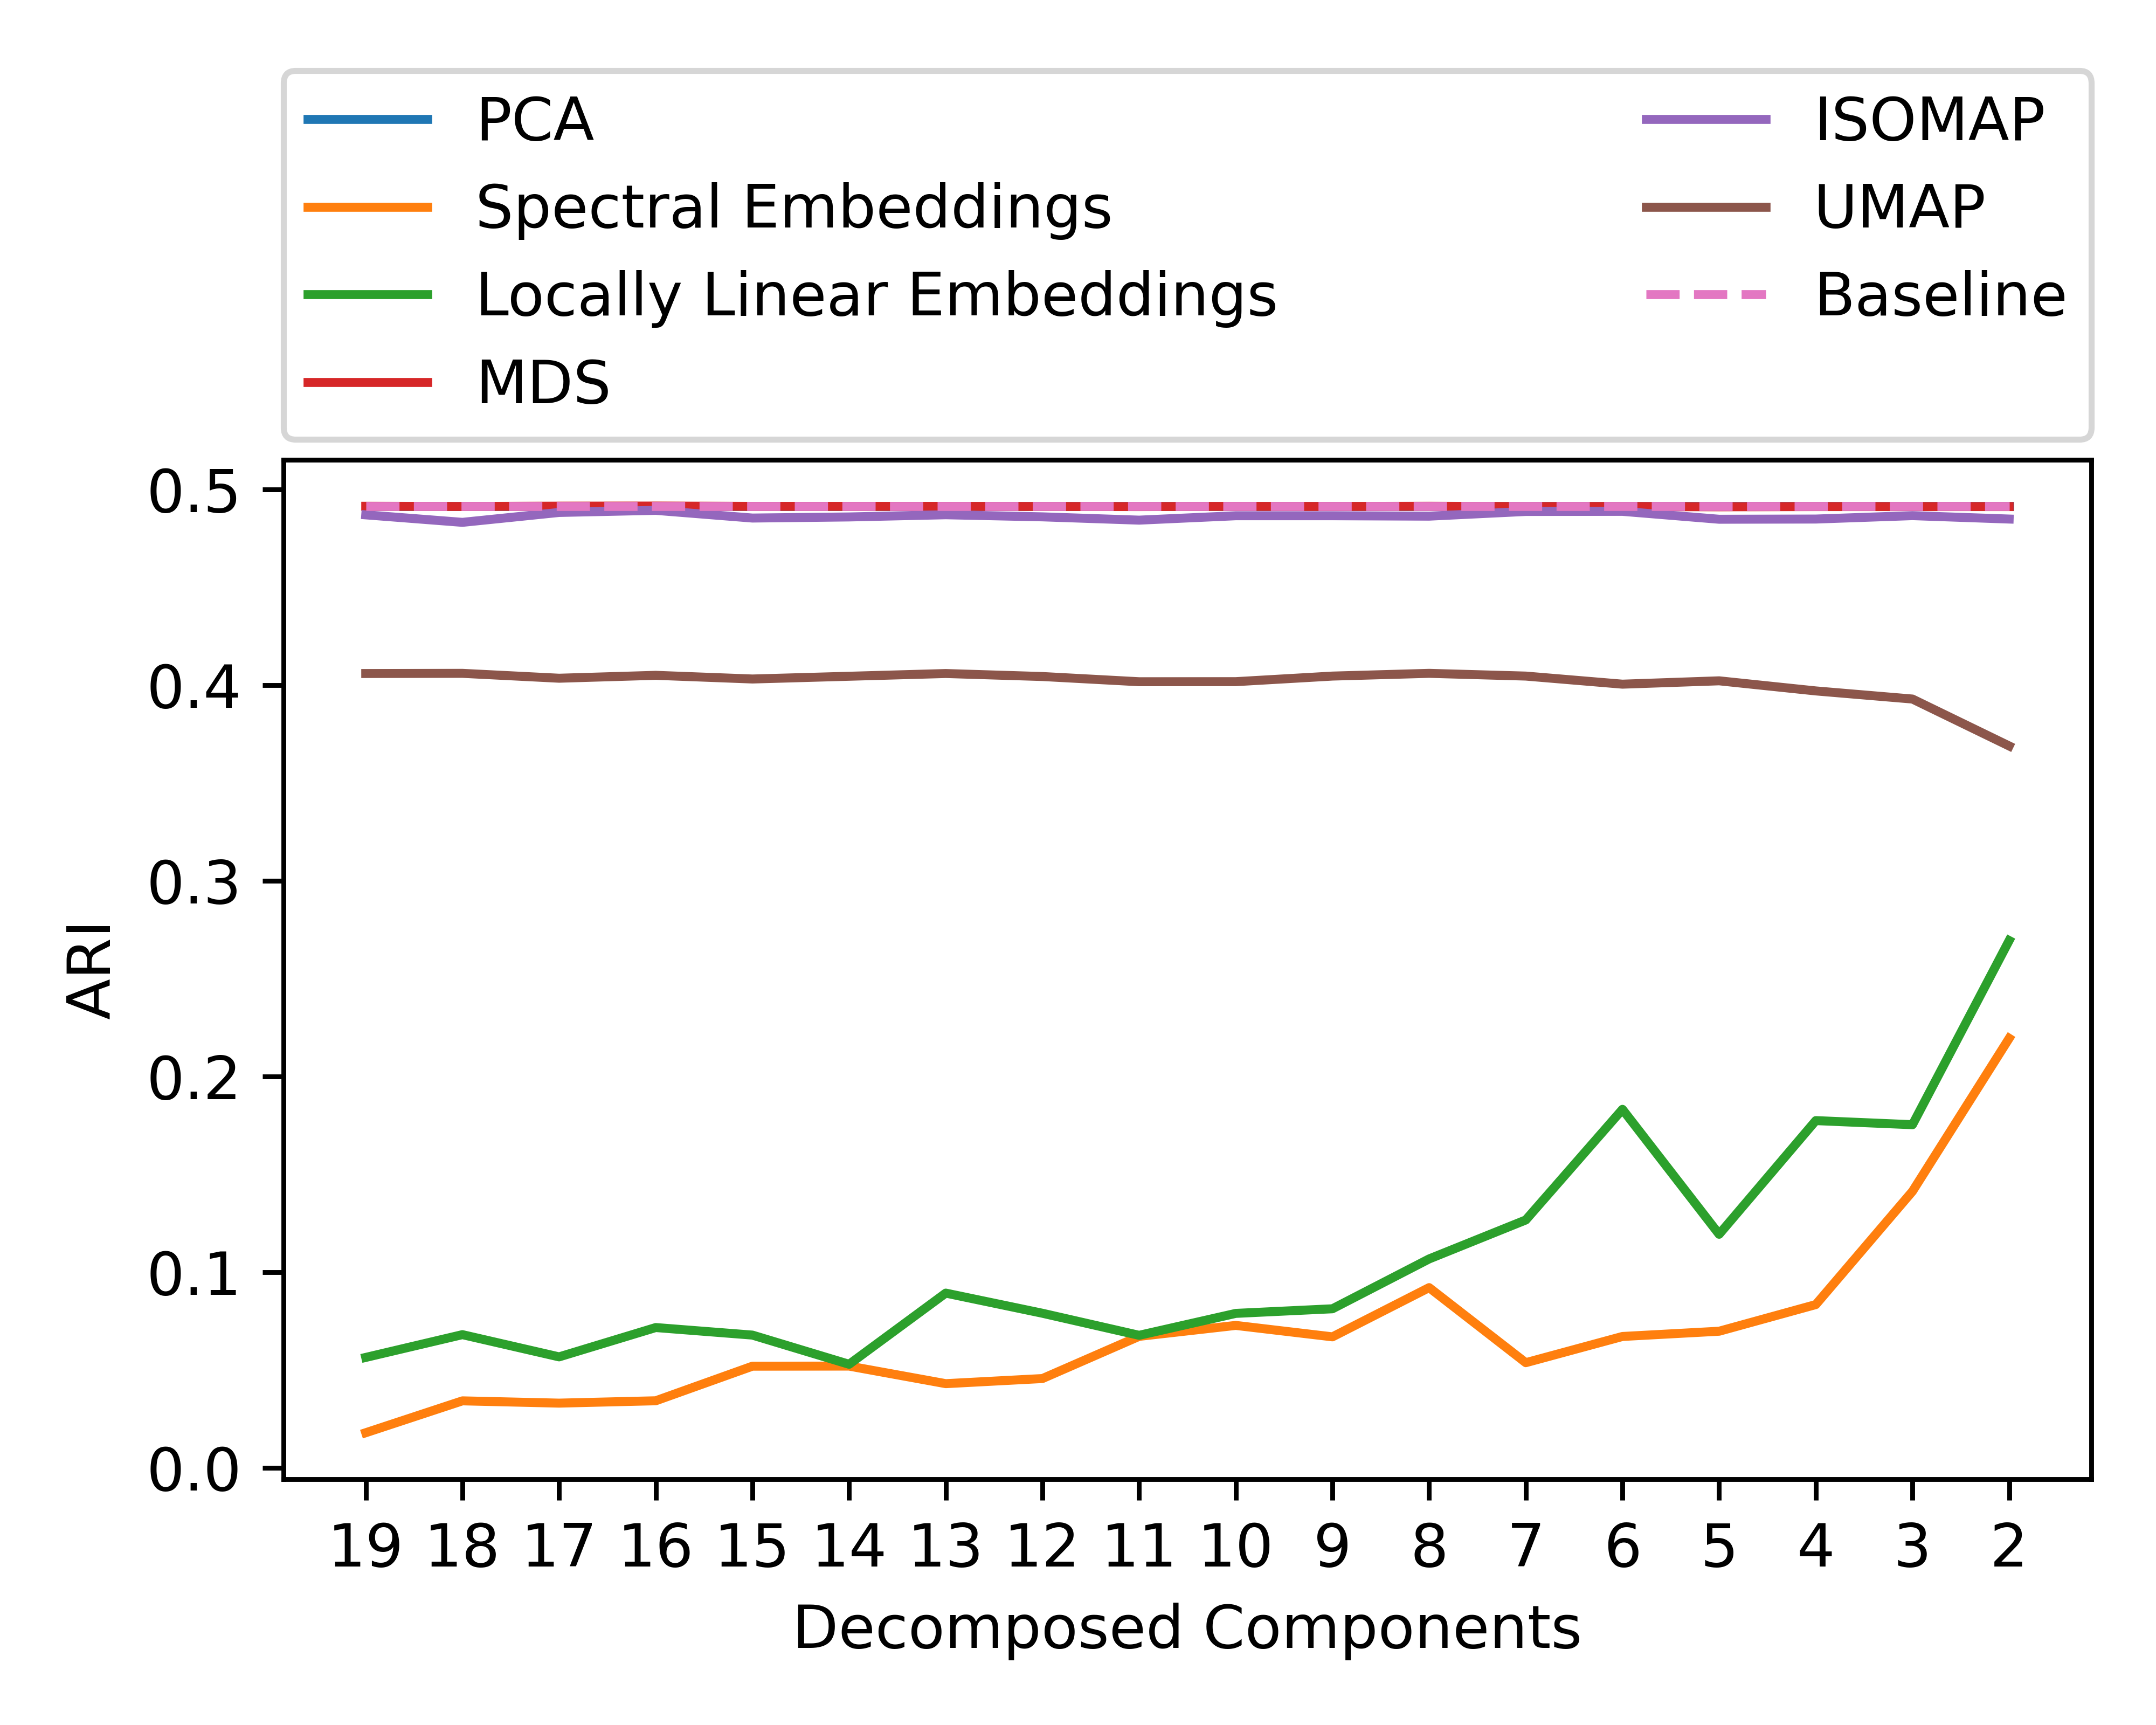
\includegraphics[width=0.48\linewidth]{images/charts_real/real_data_breast_cancer_ari.png}
                        \label{subfig:breast_cancer:ari}
                    }
                    \subfigure[]{
                        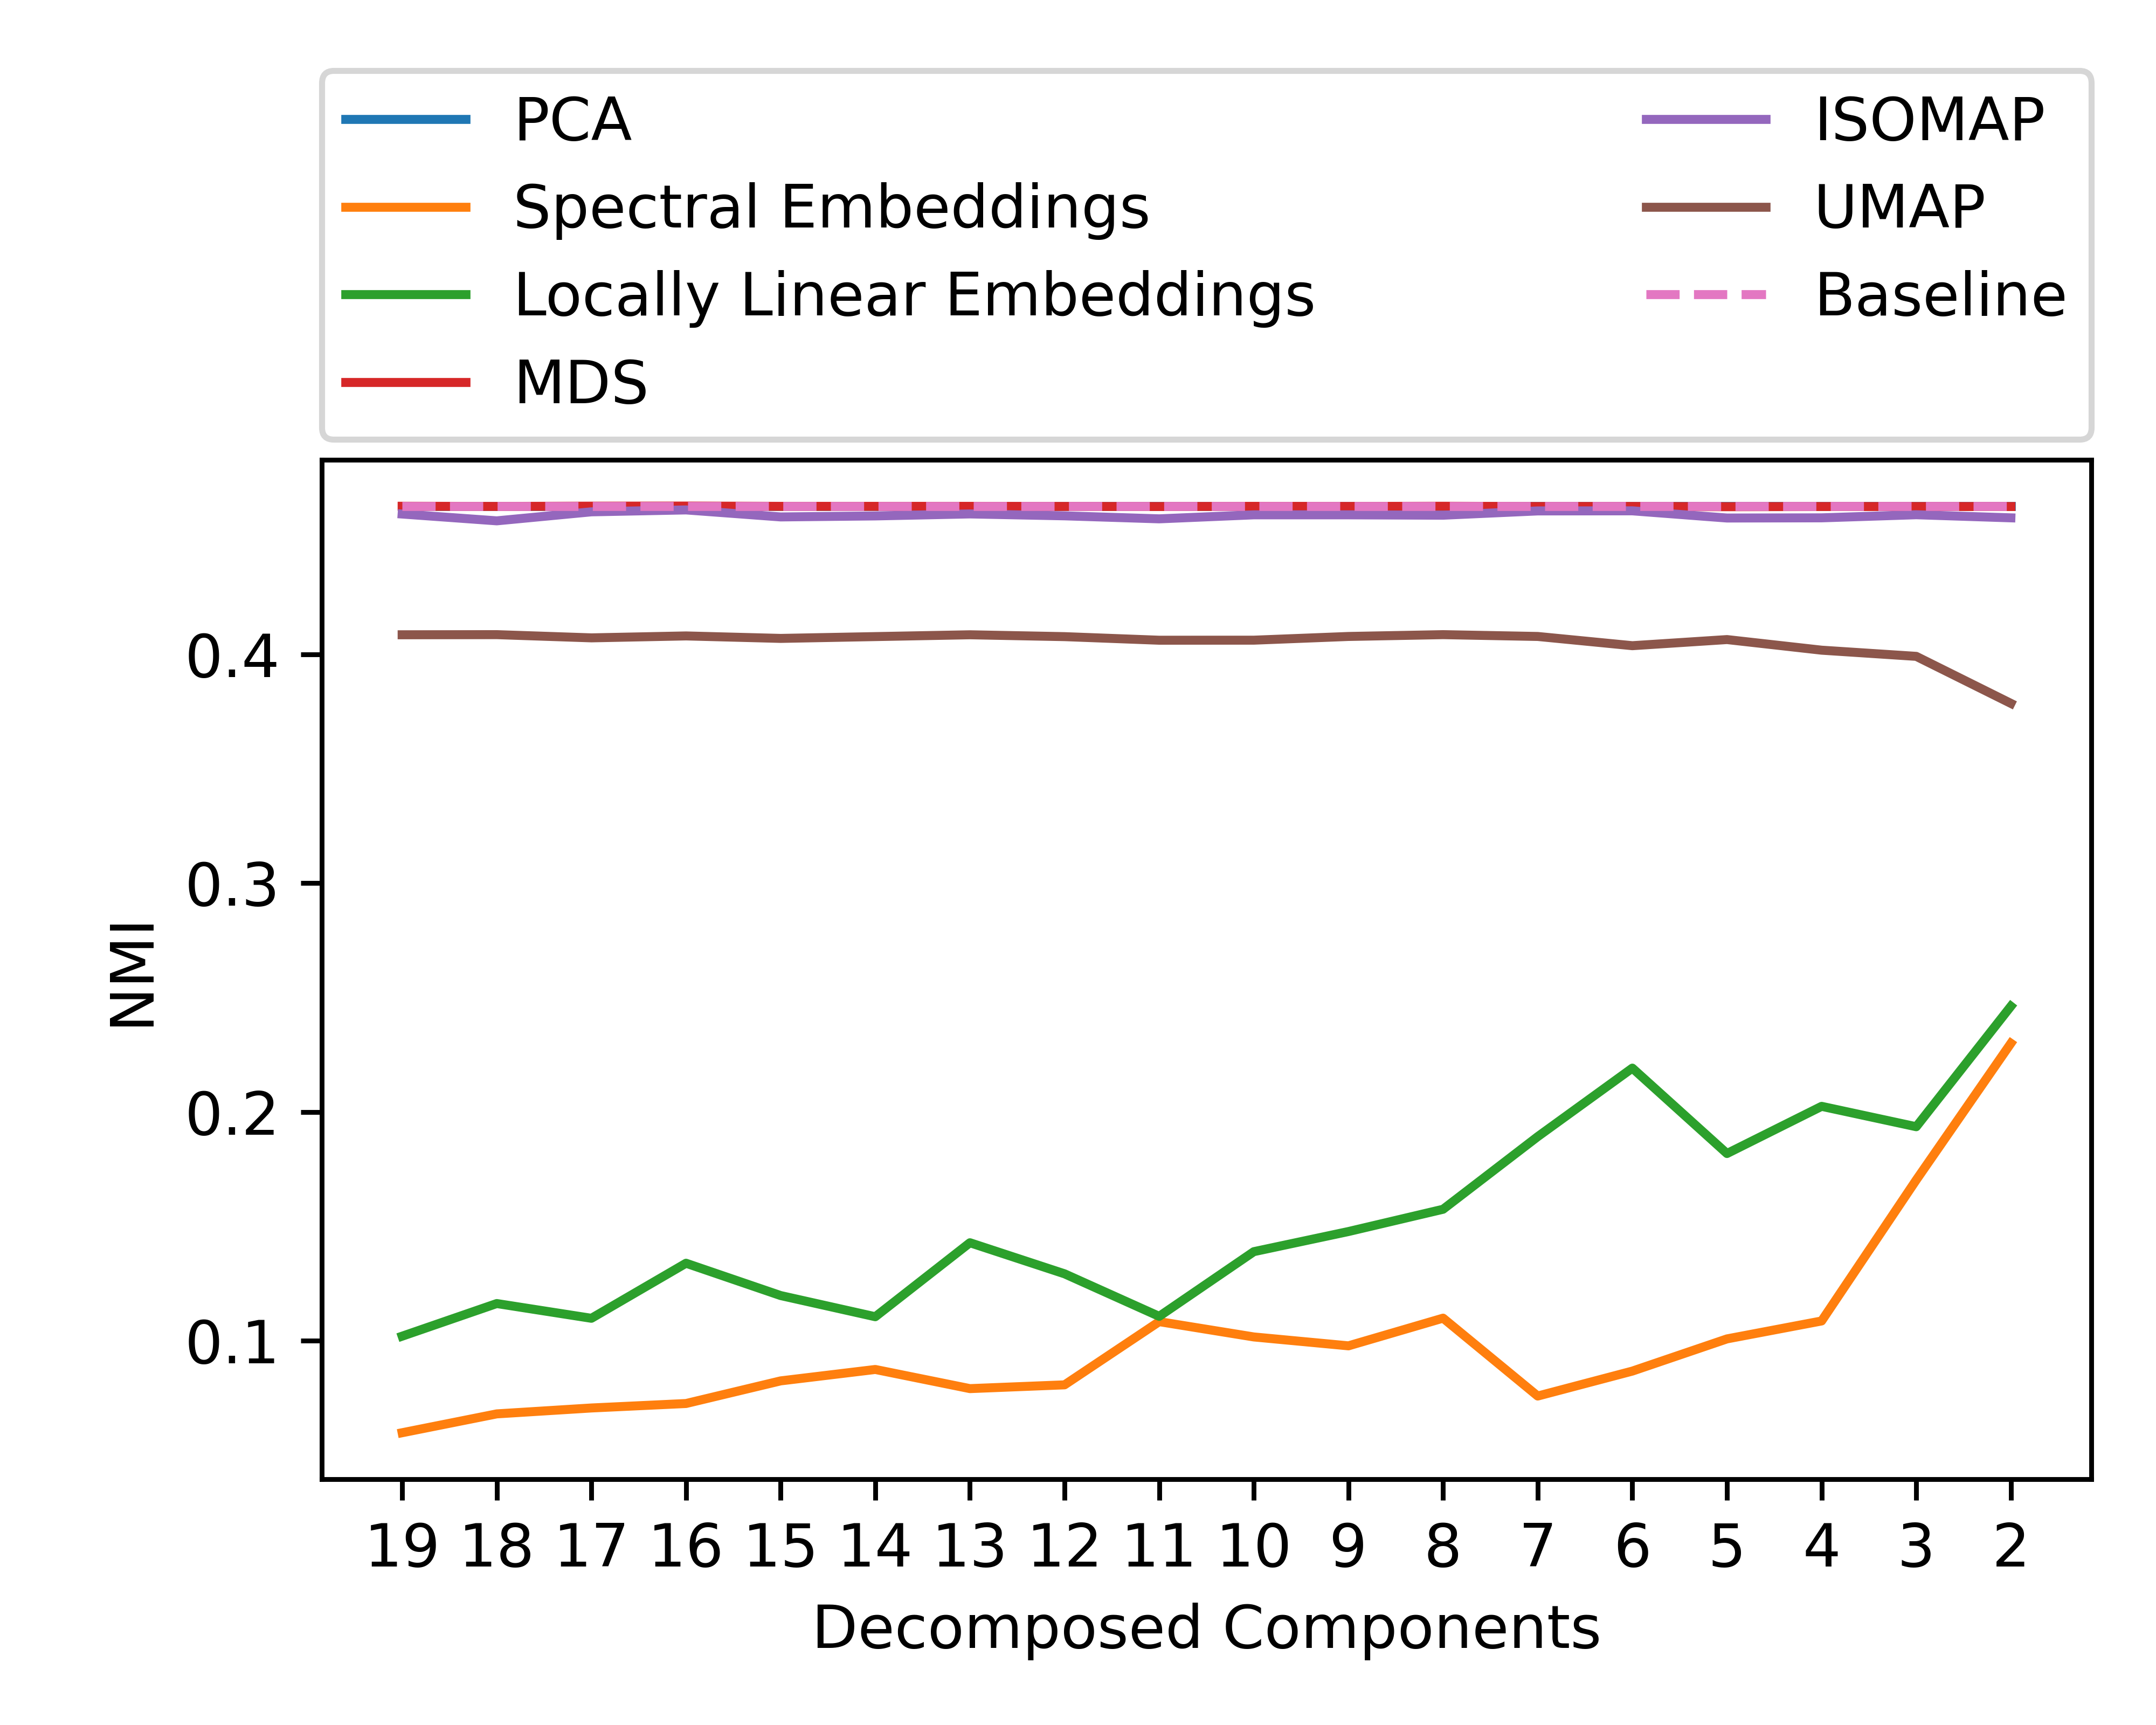
\includegraphics[width=0.48\linewidth]{images/charts_real/real_data_breast_cancer_nmi.png}
                        \label{subfig:breast_cancer:nmi}
                    }
                    \subfigure[]{
                        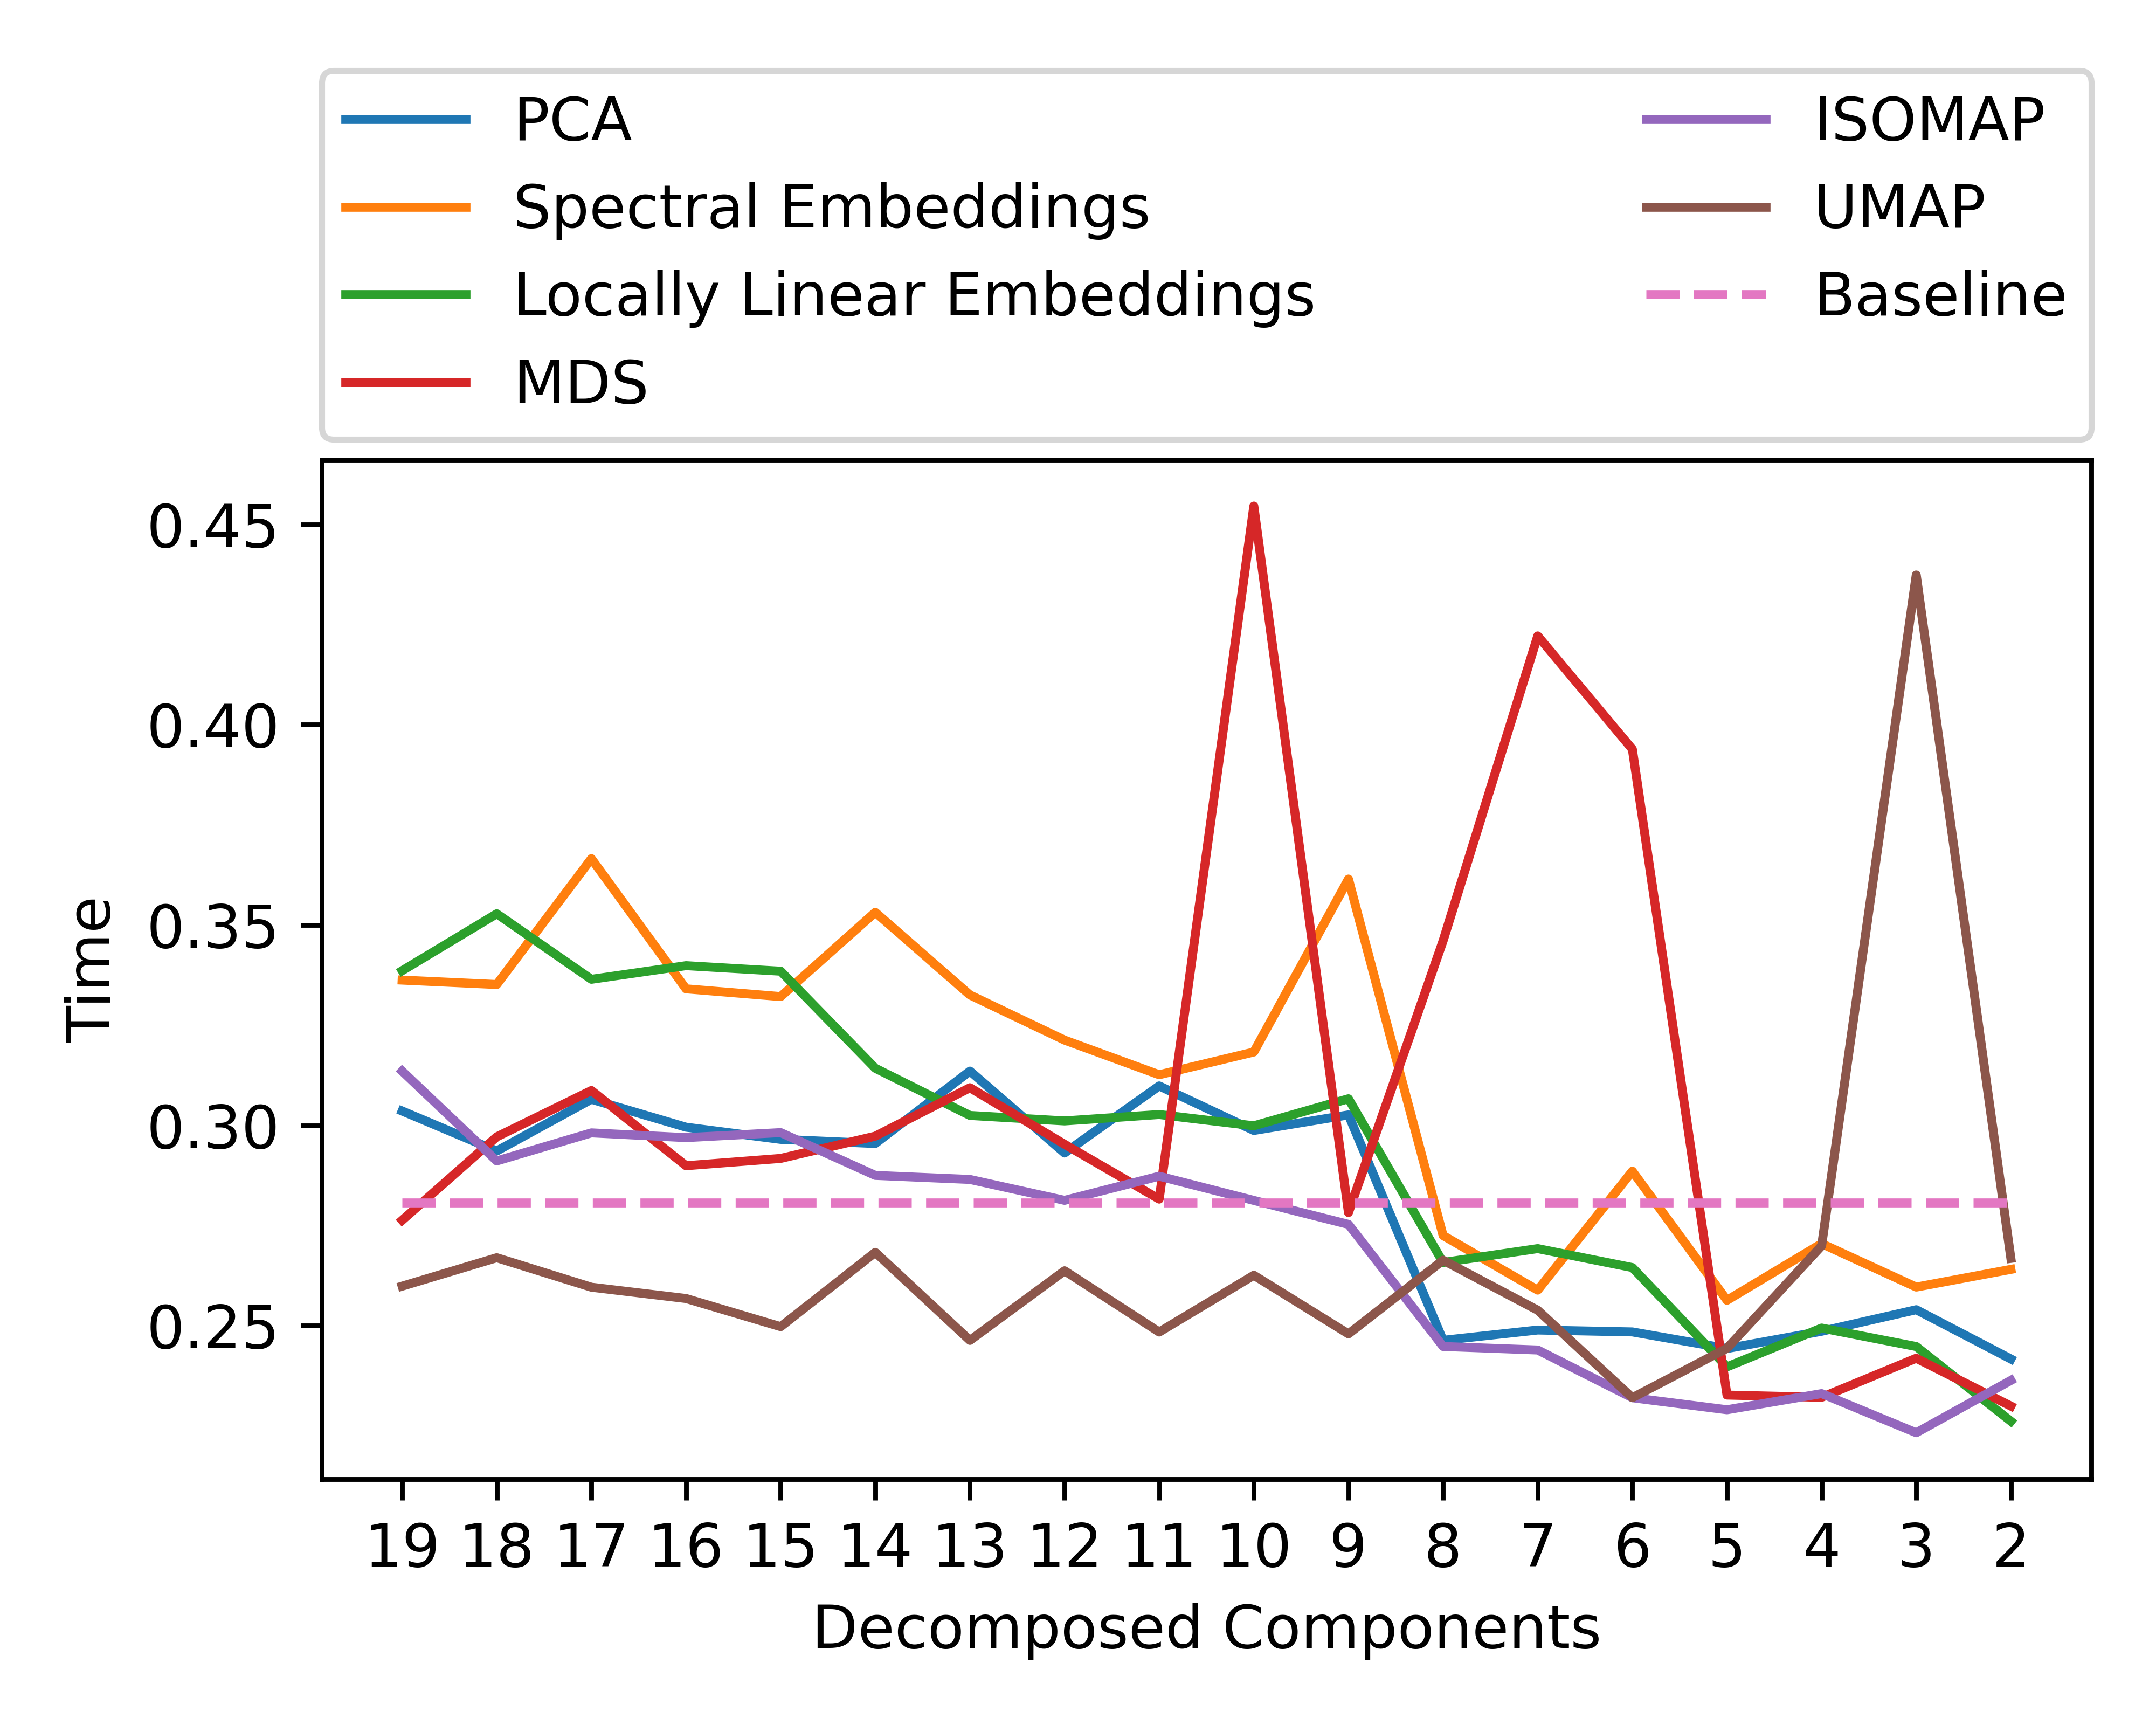
\includegraphics[width=0.48\linewidth]{images/charts_real/real_data_breast_cancer_time.png}
                        \label{subfig:breast_cancer:time}
                    }
                    \caption{Анализ влияния различных методов снижения размерности данных на кластеризацию набора данных Breast Cancer. Линия Baseline -- результат работы алгоритма \kmeans{} без предварительного снижения размерности. Результаты для
                        \subref{subfig:breast_cancer:ami} AMI;
                        \subref{subfig:breast_cancer:ari} ARI;
                        \subref{subfig:breast_cancer:nmi} NMI, а также на время работы алгоритма \subref{subfig:breast_cancer:time}.
                    }
                    \label{fig:breast_cancer}
                \end{figure}

                На рисунке \ref{fig:breast_cancer} представлены результаты применения различных методов снижения размерности перед кластеризацией K-Means на наборе данных Breast Cancer. Наиболее заметную положительную динамику продемонстрировали методы Locally Linear Embedding (LLE) и Spectral Embedding -- при уменьшении размерности до 10 и ниже наблюдается последовательный рост метрик кластеризации: AMI, ARI и NMI. Пиковые значения достигаются в точке, где число компонент совпадает с числом кластеров в выборке, что может свидетельствовать о более точной структурной декомпозиции, когда размерность пространства отражает истинное количество скрытых групп. В то же время алгоритмы PCA и MDS демонстрируют стабильные показатели качества, близкие к базовому сценарию кластеризации без предварительного снижения размерности. Это указывает на то, что оба метода хорошо сохраняют глобальную структуру данных, которая является ключевой для работы алгоритма K-Means. Особенно стоит отметить MDS, который обеспечивает не только стабильность качества, но и высокую воспроизводимость результатов на всем диапазоне размерностей. Такое поведение подтверждает различия в подходах: методы LLE и Spectral Embedding склонны акцентировать внимание на локальных взаимосвязях между точками, что делает их полезными при сильной редукции, в то время как PCA и MDS сохраняют глобальную топологию, важную для более устойчивой кластеризации.

            \paragraph{Результаты алгоритма на наборе данных Digits.}
                Digits — это стандартный набор данных для многоклассовой классификации, часто используемый в задачах распознавания образов. Данные представляют собой рукописные цифры от 0 до 9, оцифрованные в виде изображений 8x8 пикселей. Каждое изображение преобразовано в матрицу чисел, отражающих интенсивность оттенков серого.

                \begin{table}[H]
                    \centering
                    \caption{Характеристики набора данных Digits.}
                    \begin{tabular}{ccc}
                        \toprule
                        Число классов & Число объектов & Размерность пространства \\
                        \midrule
                        10 & 1797 & 64 \\
                        \bottomrule
                    \end{tabular}
                \end{table}

                Набор данных Digits представляет собой матрицу размерностью 1797x64, где каждая строка соответствует одному изображению цифры, а каждый столбец содержит значение яркости пикселя (от 0 до 16). Исходные изображения были нормализованы для уменьшения влияния вариаций наклона и толщины линий.

                \begin{figure}[H]\centering
                    \subfigure[]{
                        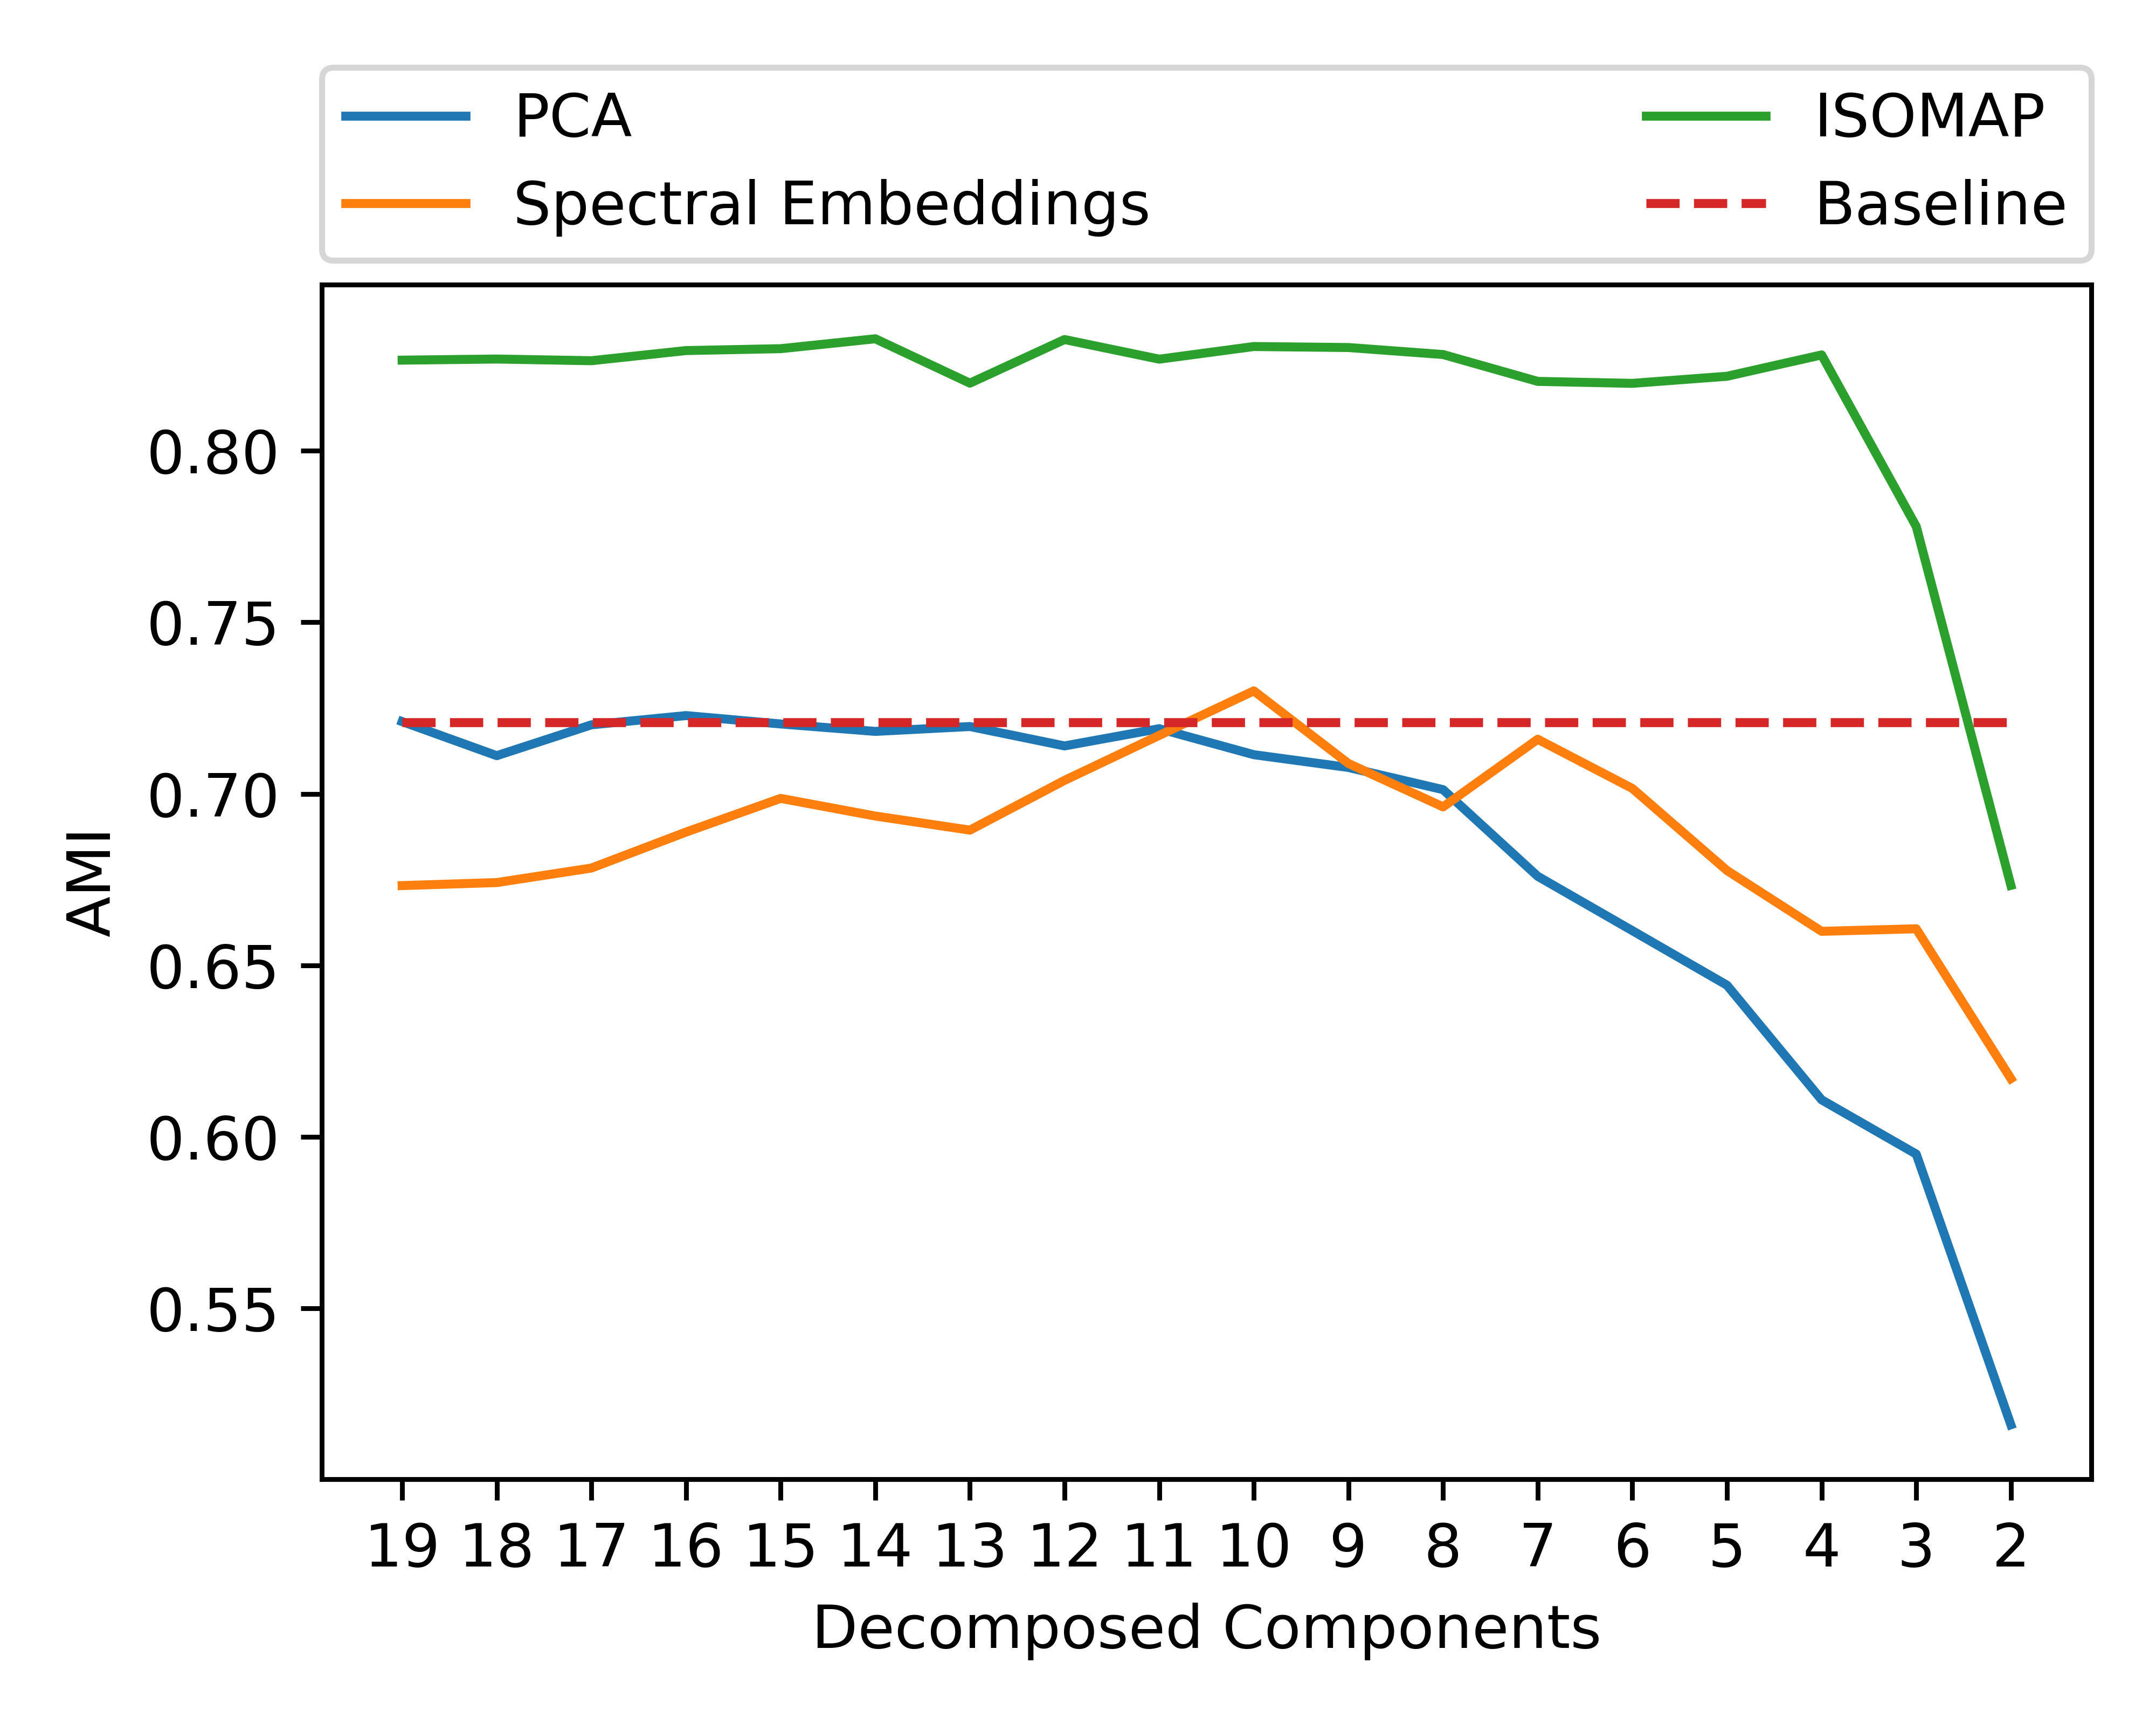
\includegraphics[width=0.48\linewidth]{images/charts_real/real_data_digits_ami.png}
                        \label{subfig:digits:ami}
                    }
                    \subfigure[]{
                        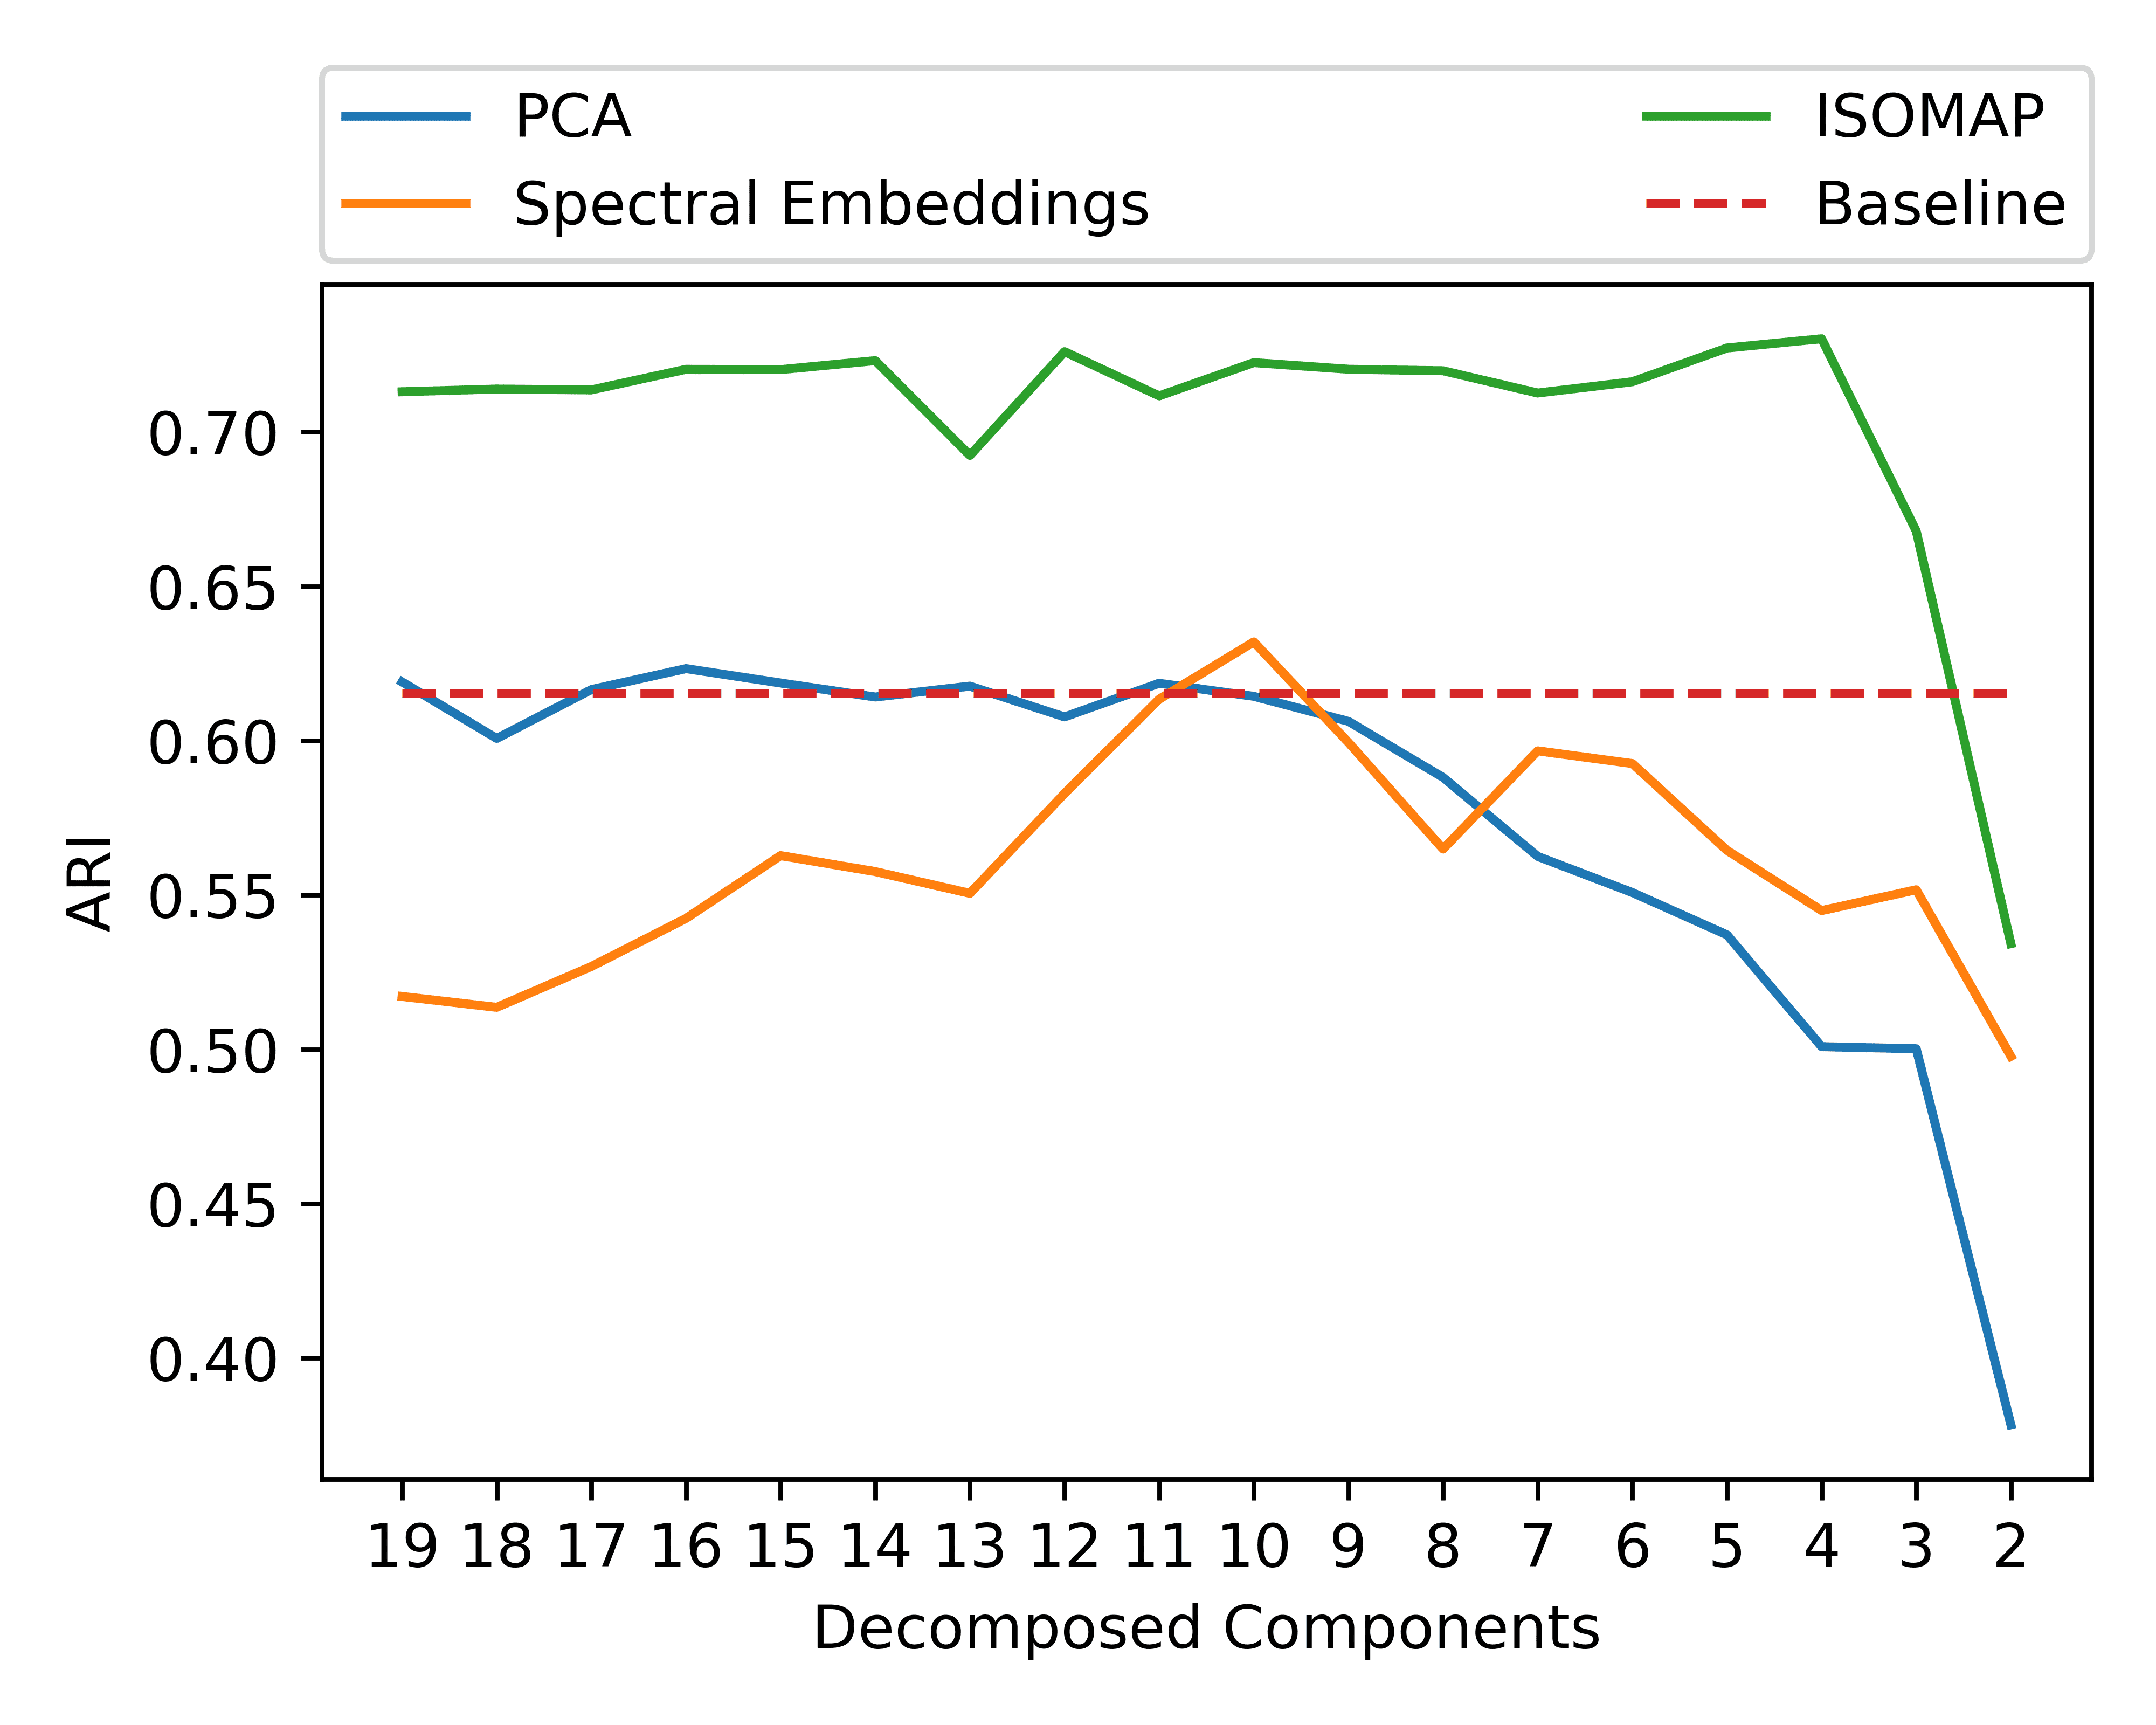
\includegraphics[width=0.48\linewidth]{images/charts_real/real_data_digits_ari.png}
                        \label{subfig:digits:ari}
                    }
                    \subfigure[]{
                        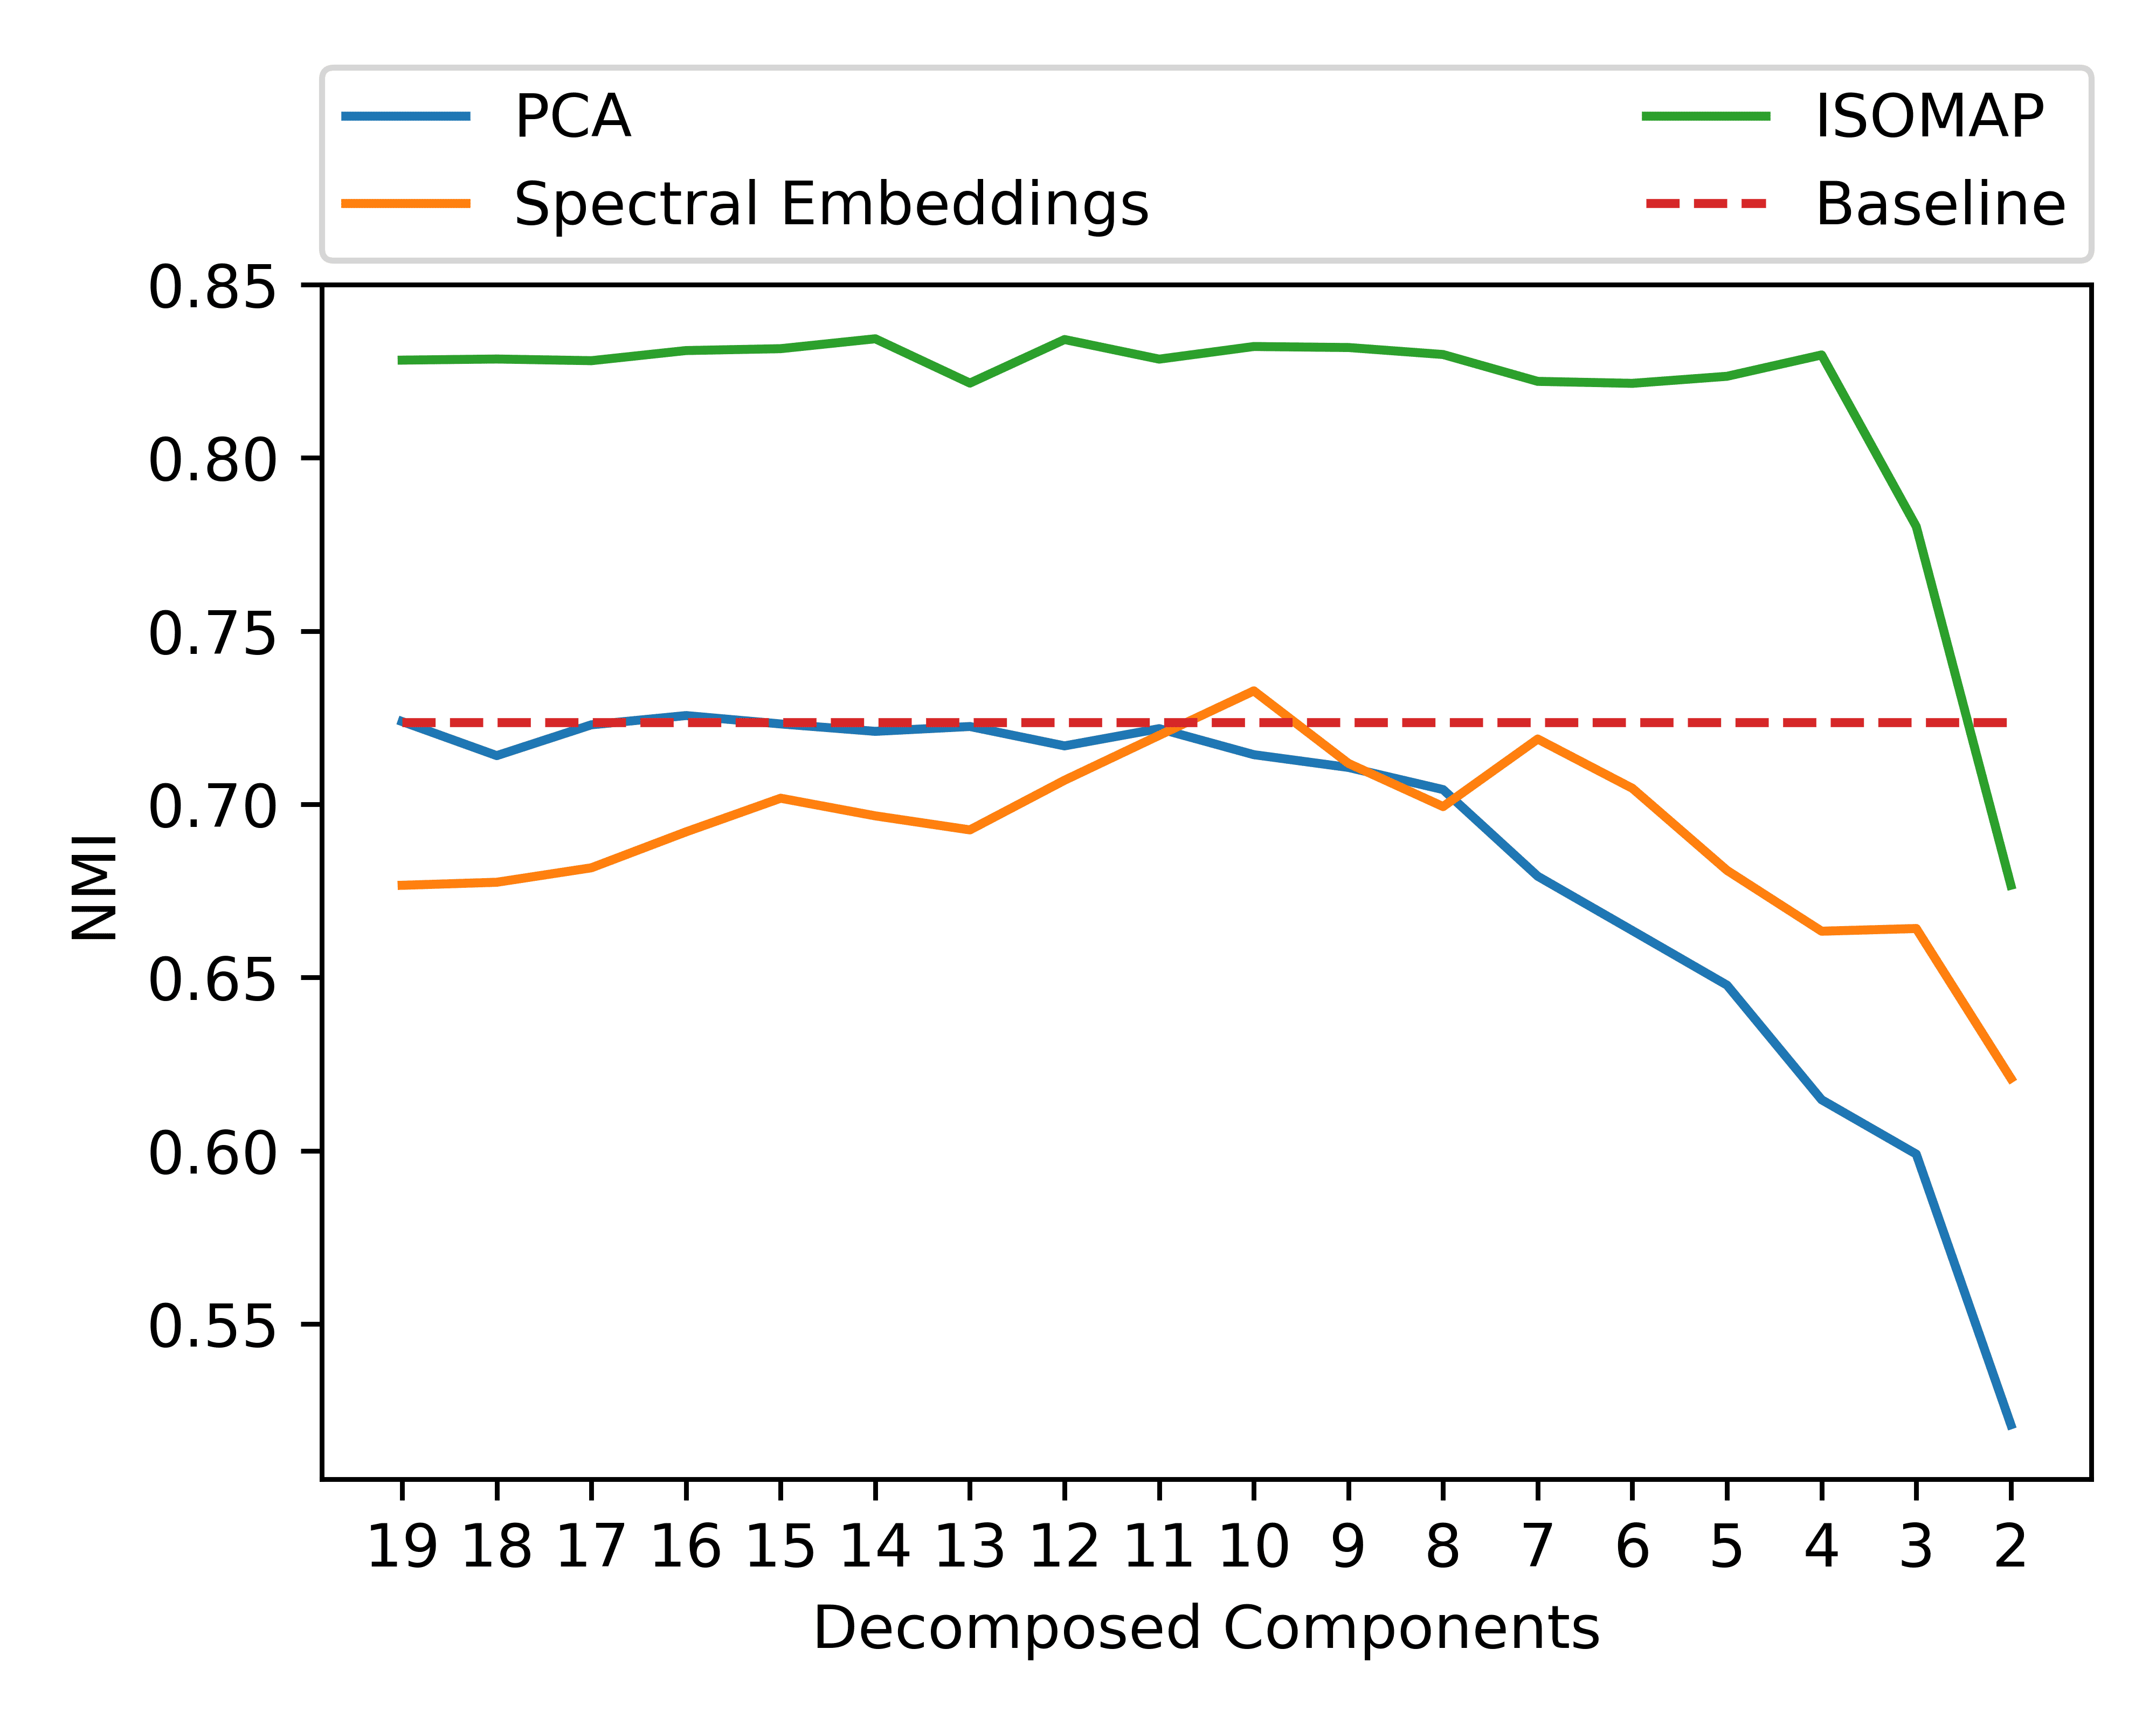
\includegraphics[width=0.48\linewidth]{images/charts_real/real_data_digits_nmi.png}
                        \label{subfig:digits:nmi}
                    }
                    \subfigure[]{
                        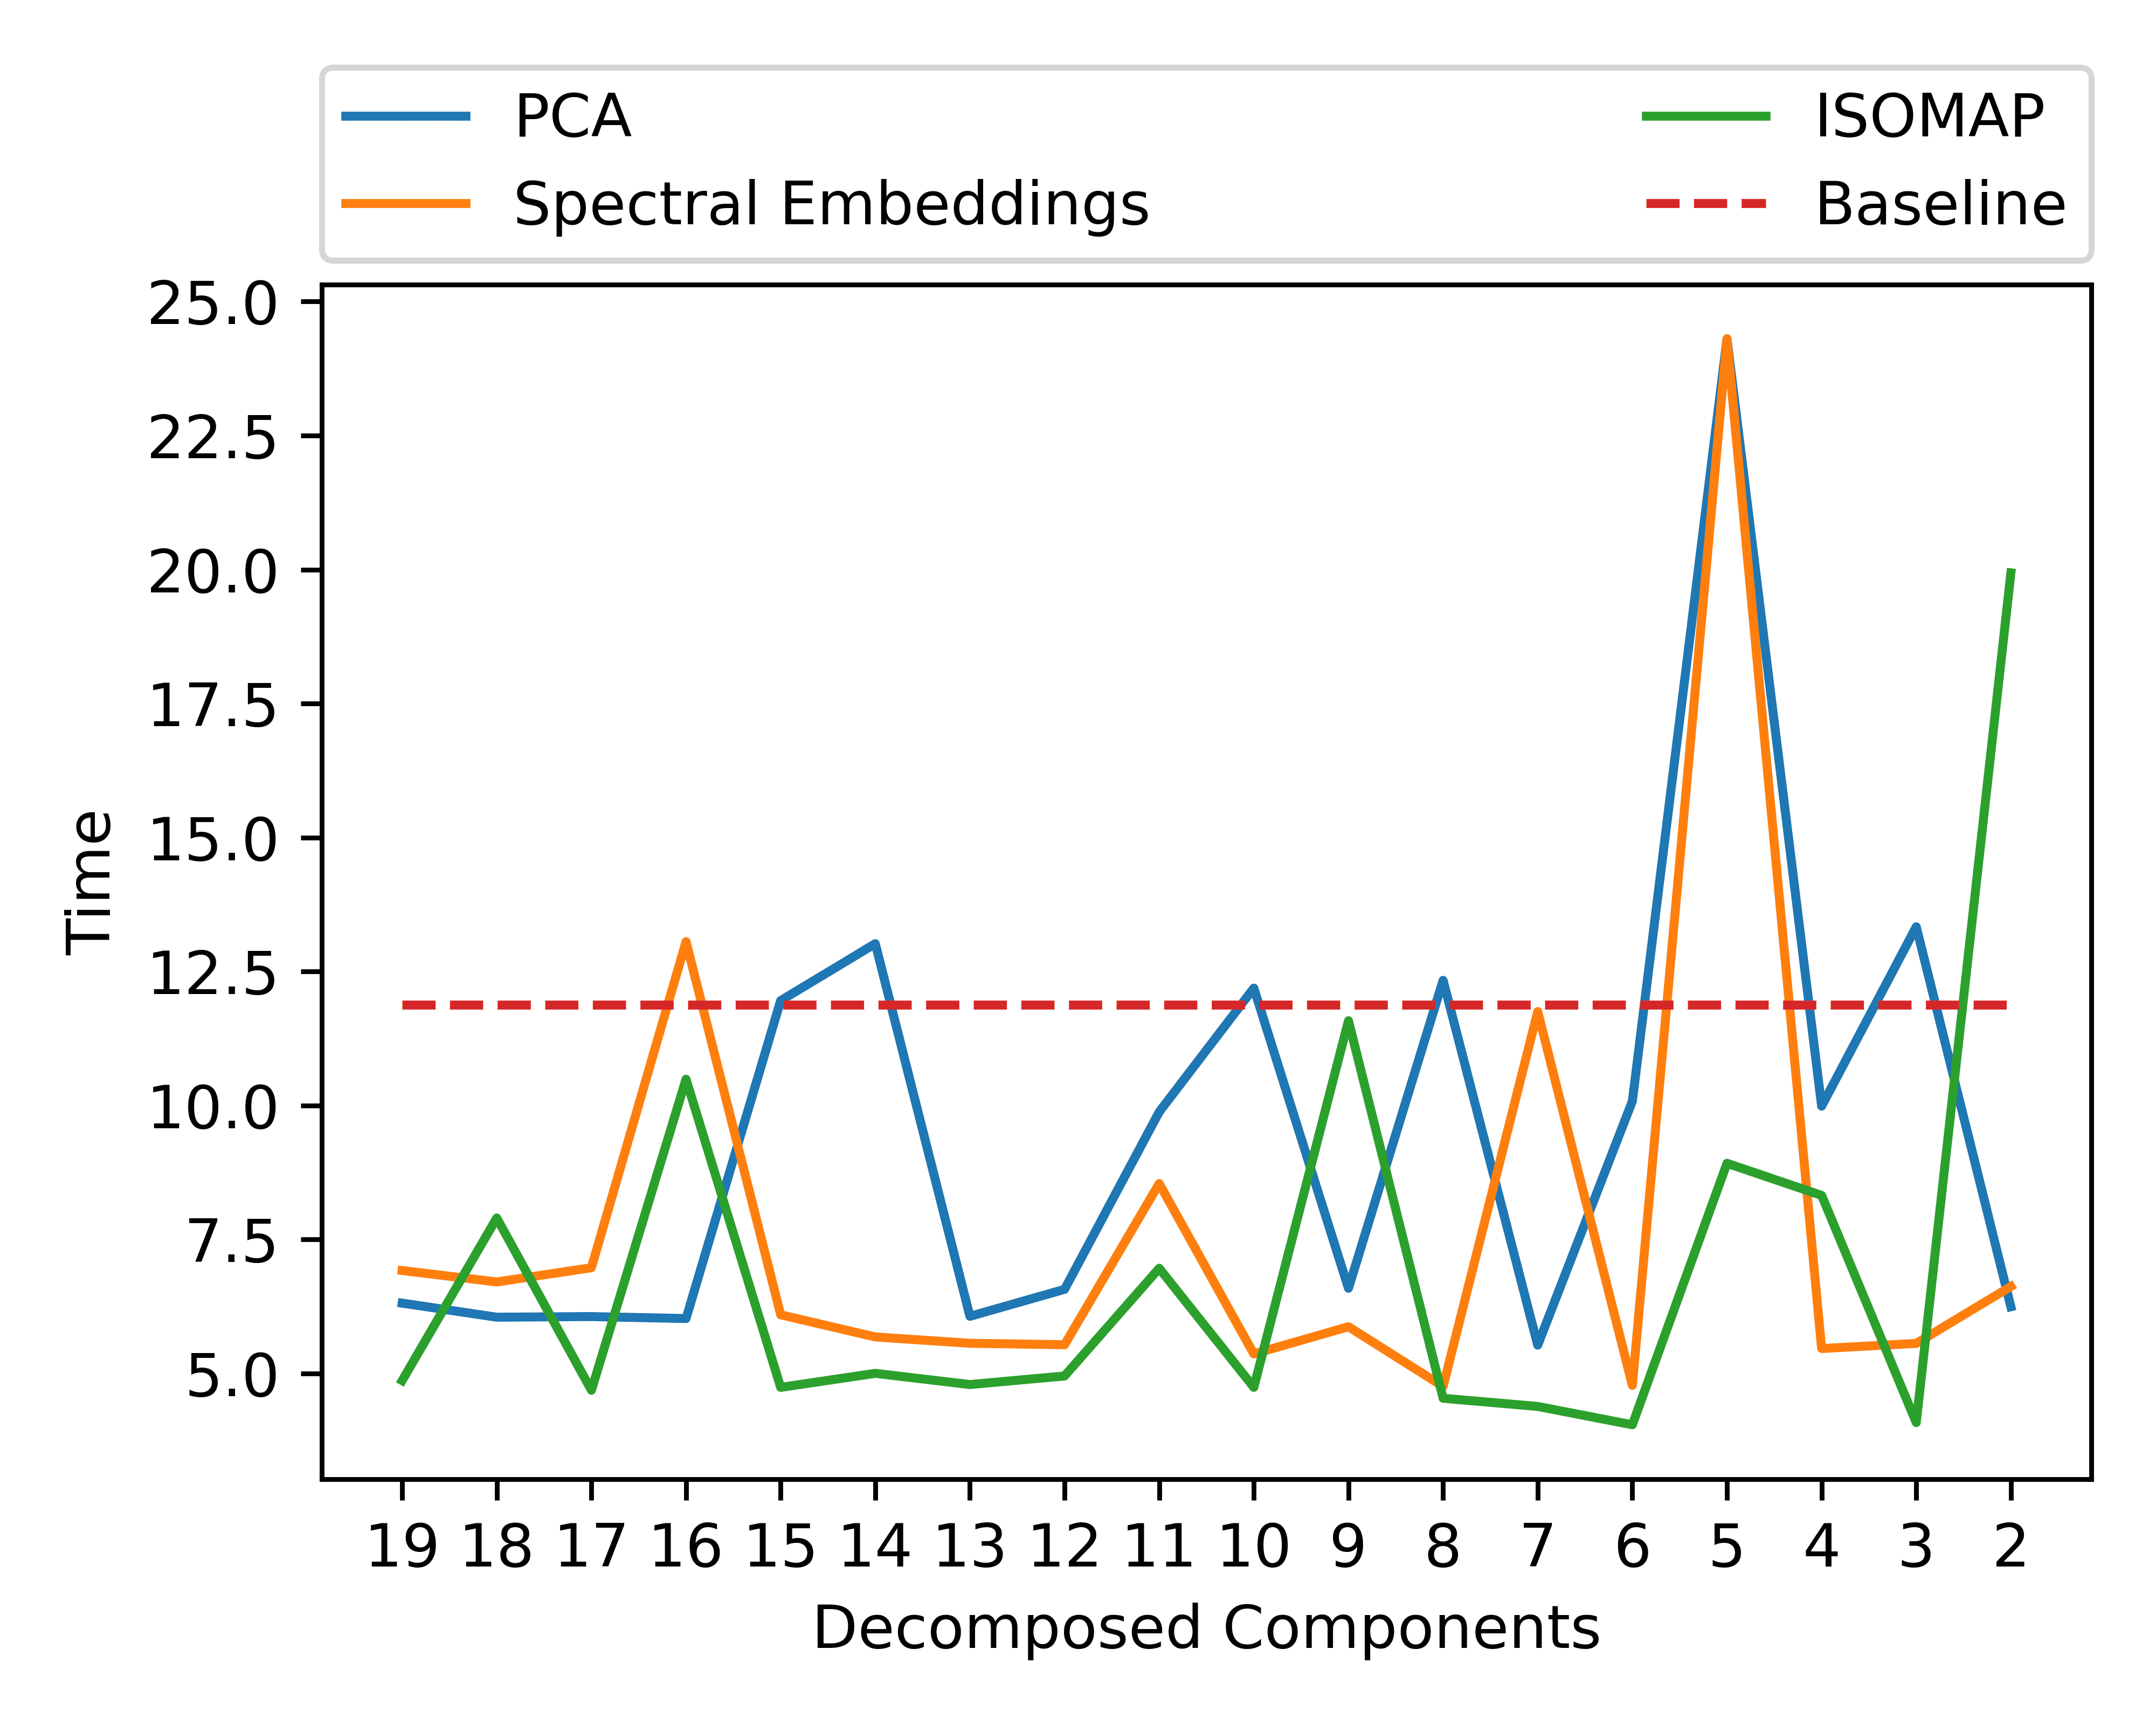
\includegraphics[width=0.48\linewidth]{images/charts_real/real_data_digits_time.png}
                        \label{subfig:digits:time}
                    }
                    \caption{Анализ влияния различных методов снижения размерности данных на кластеризацию набора данных Digits. Линия Baseline -- результат работы алгоритма \kmeans{} без предварительного снижения размерности. Результаты для
                        \subref{subfig:digits:ami} AMI;
                        \subref{subfig:digits:ari} ARI;
                        \subref{subfig:digits:nmi} NMI, а также на время работы алгоритма \subref{subfig:digits:time}.
                    }
                    \label{fig:digits}
                \end{figure}

                На рисунке \ref{fig:digits} представлены результаты экспериментов на датасете Digits. Следует отметить, что из-за ограничений существующей программной реализации методы MDS и Locally Linear Embedding не смогли корректно выполнить процедуру снижения размерности на этом наборе данных и, таким образом, были исключены из анализа. Среди протестированных алгоритмов ярким лидером оказался ISOMAP, который уверенно превзошёл остальные методы по всем основным метрикам кластеризации — AMI, ARI и NMI. Он продемонстрировал стабильное превосходство над базовой линией (результат кластеризации без снижения размерности) вплоть до размерности в 2 компоненты, что говорит о его способности сохранять глобальную геометрию данных даже в сильно сжатом пространстве. Метод PCA продемонстрировал устойчивую деградацию качества кластеризации при уменьшении числа компонент, особенно заметную ниже порога в 10 компонент. Это отражает его ограниченность в улавливании нелинейных зависимостей в данных. Spectral Embedding, напротив, показал результаты в целом ниже уровня базового \kmeans{}, что может объясняться тем, что он оптимизирует локальные отношения между точками, а не глобальную структуру. Тем не менее, на размерности, равной числу кластеров, наблюдался кратковременный всплеск метрик, что, вероятно, связано с тем, что алгоритм эффективно извлекает локальные кластеры, когда размерность достаточно для сохранения этих структур. Также была выявлена интересная зависимость по времени выполнения: ISOMAP, несмотря на свою сложность, в среднем демонстрировал сравнительно низкое время работы с редкими всплесками, что делает его не только точным, но и потенциально пригодным для практического применения при разумной конфигурации.

            \paragraph{Результаты алгоритма на наборе данных Wine.}
                Wine - это стандартный и простой набор данных для многоклассовой классификации. Эти данные являются результатами химического анализа вин, выращенных в одном и том же регионе Италии тремя разными производителями. Существует тринадцать различных измерений, проведенных для различных компонентов, содержащихся в трех сортах вина.

                \begin{table}[H]
                    \centering
                    \caption{Характеристики набора данных Wine.}
                    \begin{tabular}{ccc}
                        \toprule
                        Число классов &   Число объектов &   Размерность пространства \\
                        \midrule
                        3    &  178 &  13 \\
                        \bottomrule
                    \end{tabular}
                \end{table}

                Набор данных Wine представляет собой матрицу с размерностью 178x13, где каждая строка соответствует отдельному образцу вина, а каждый столбец содержит значение конкретного химического измерения.

                \begin{figure}[H]\centering
                    \subfigure[]{
                        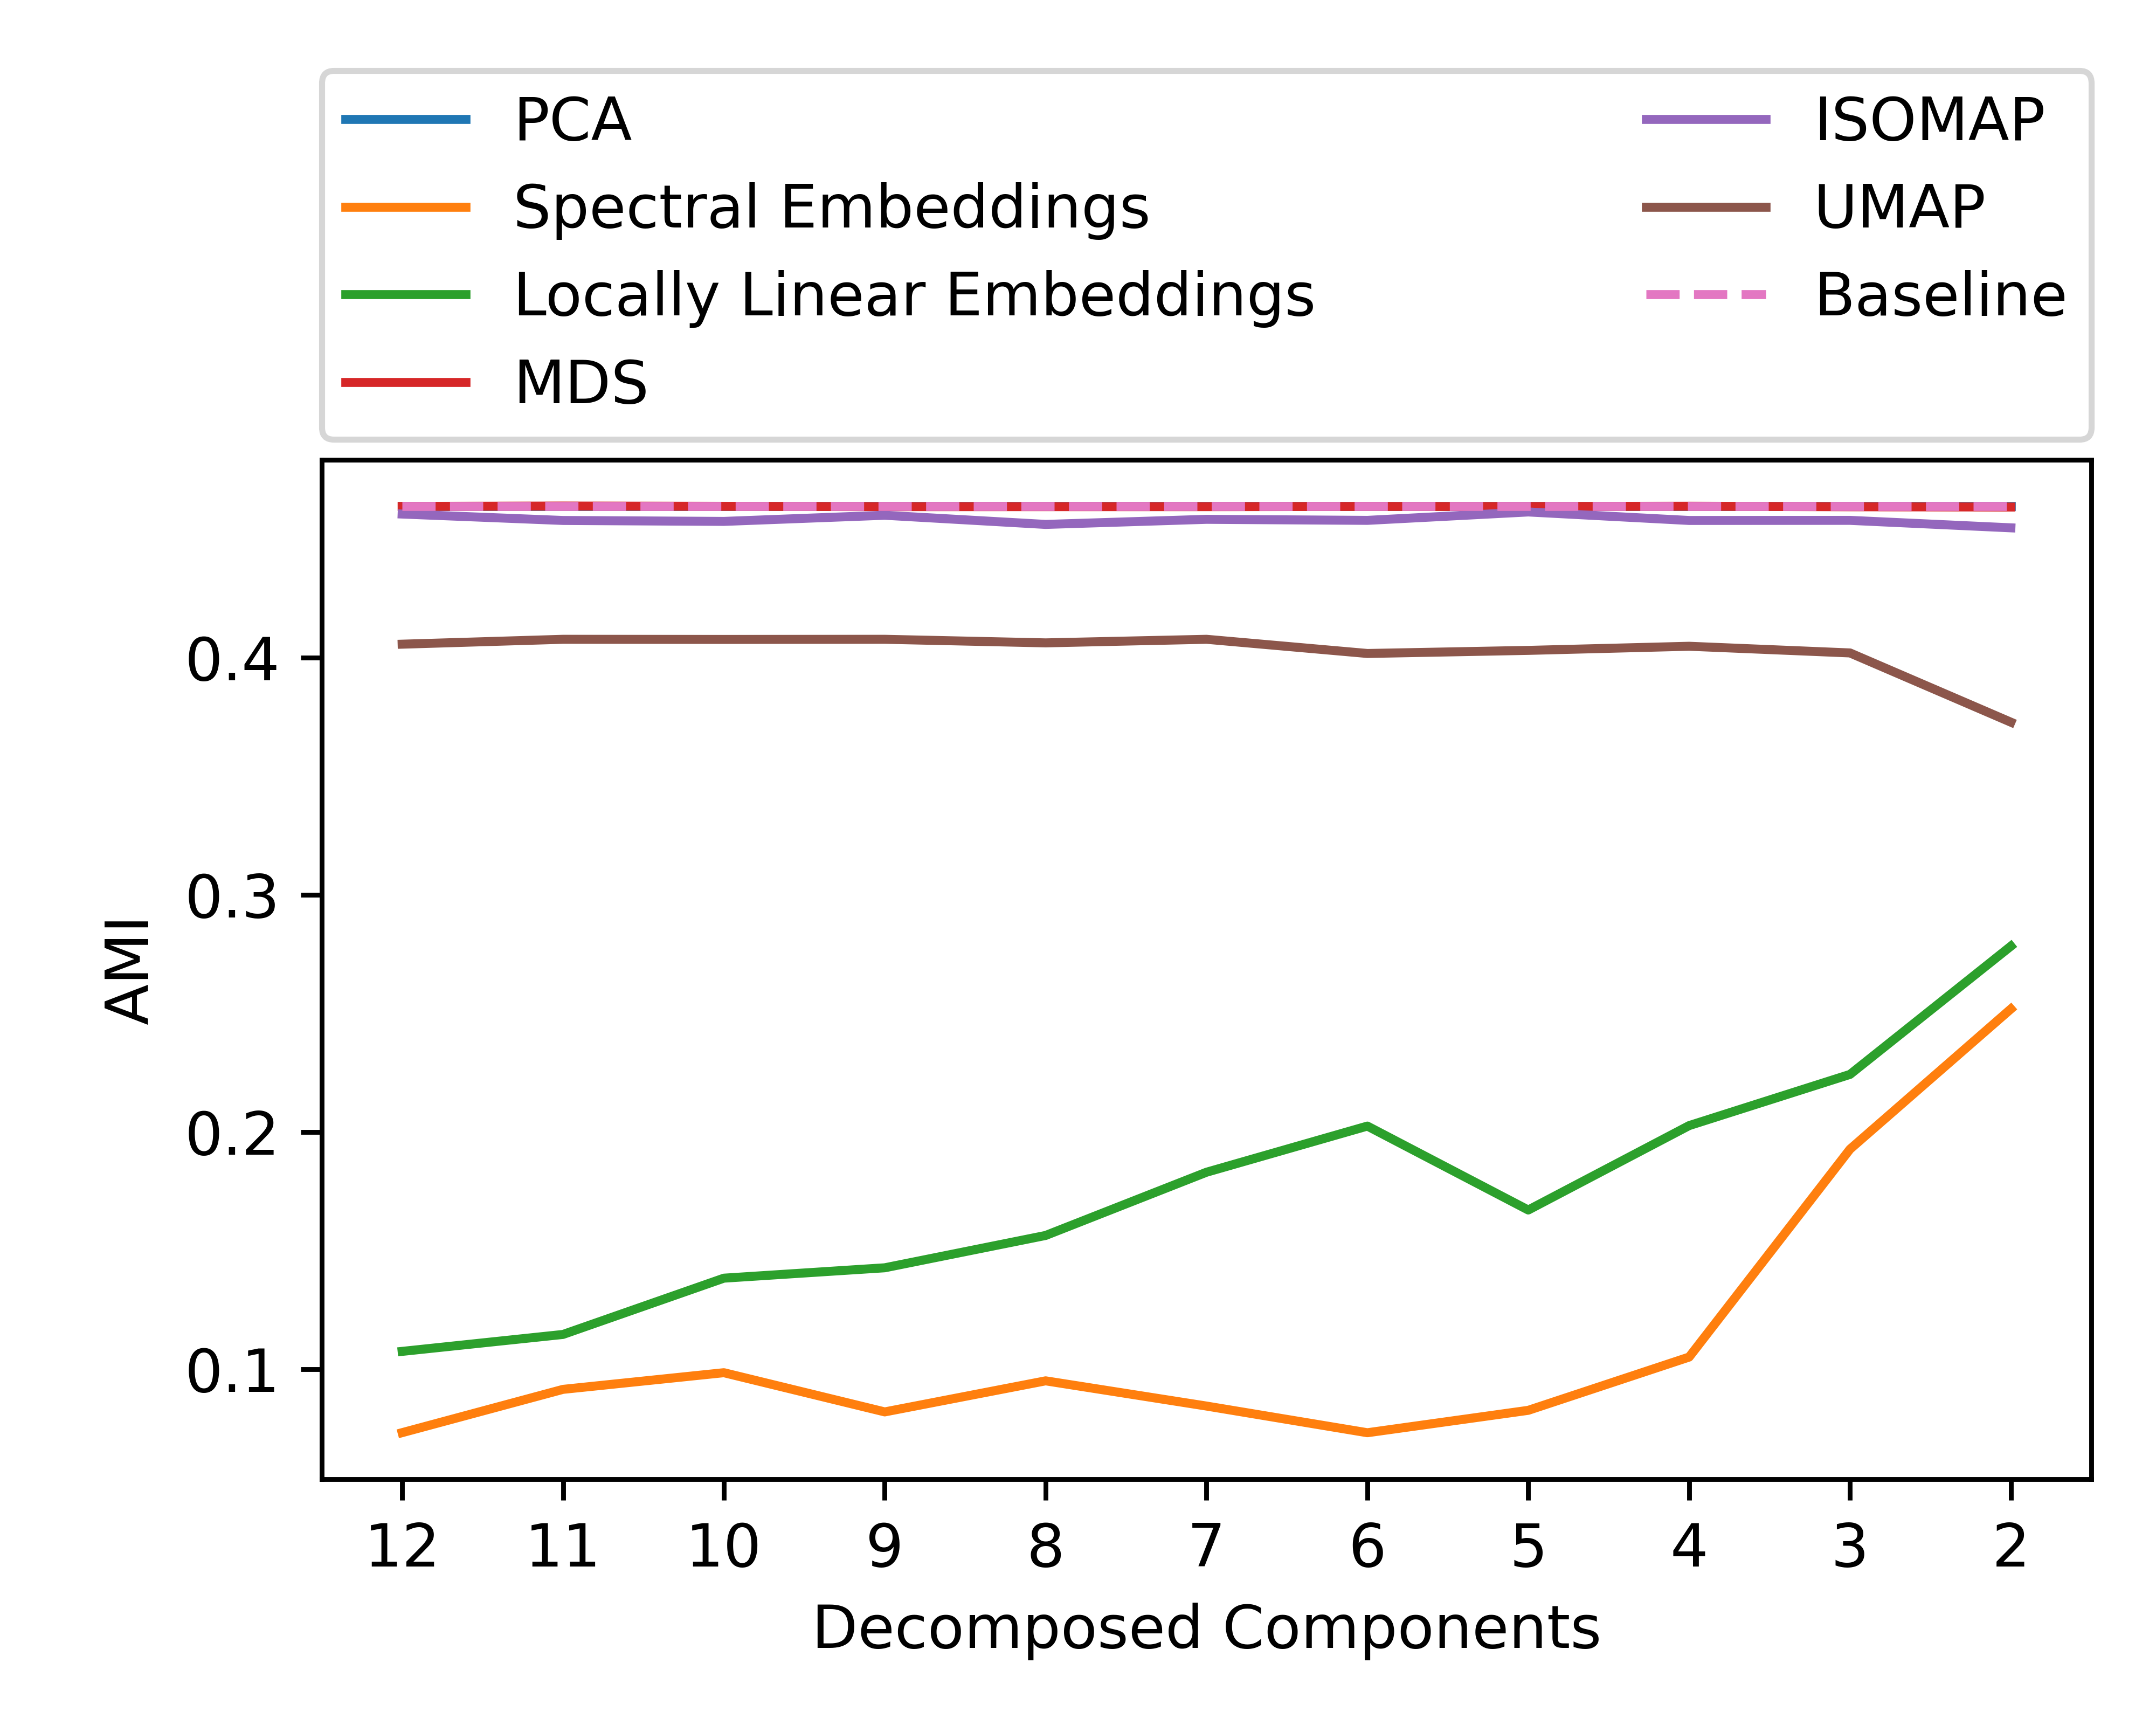
\includegraphics[width=0.48\linewidth]{images/charts_real/real_data_wine_ami.png}
                        \label{subfig:wine:ami}
                    }
                    \subfigure[]{
                        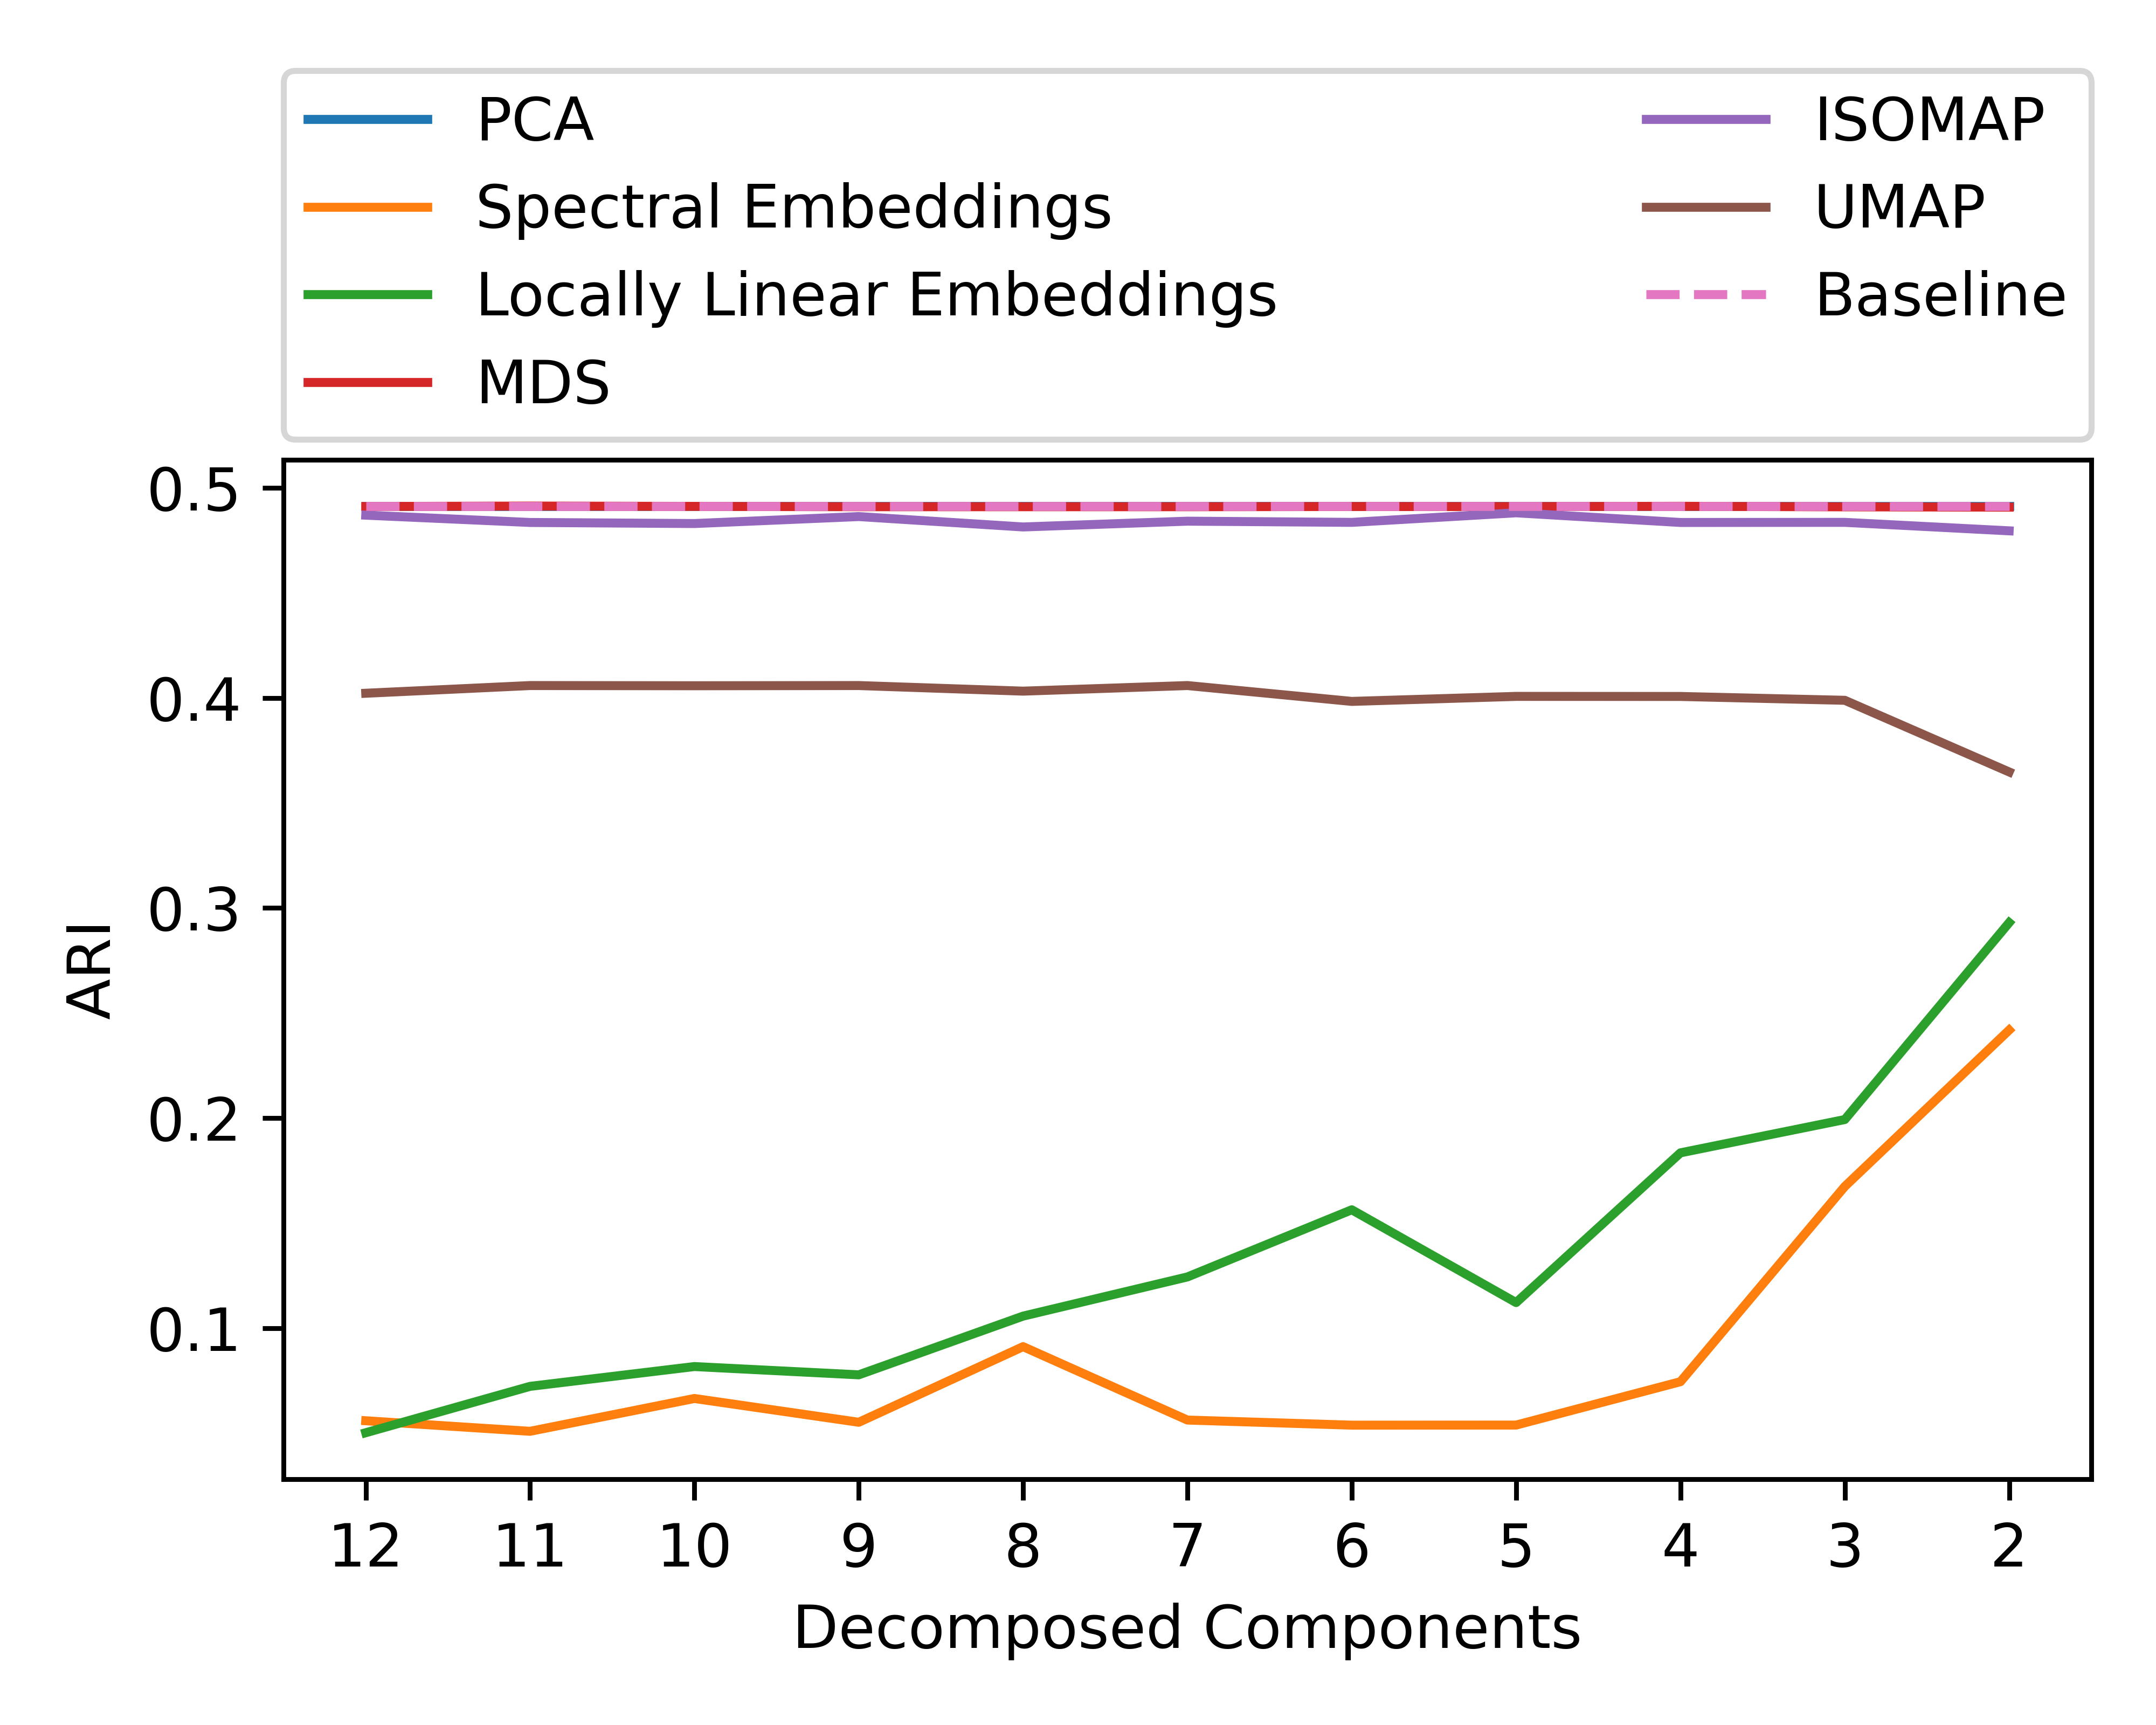
\includegraphics[width=0.48\linewidth]{images/charts_real/real_data_wine_ari.png}
                        \label{subfig:wine:ari}
                    }
                    \subfigure[]{
                        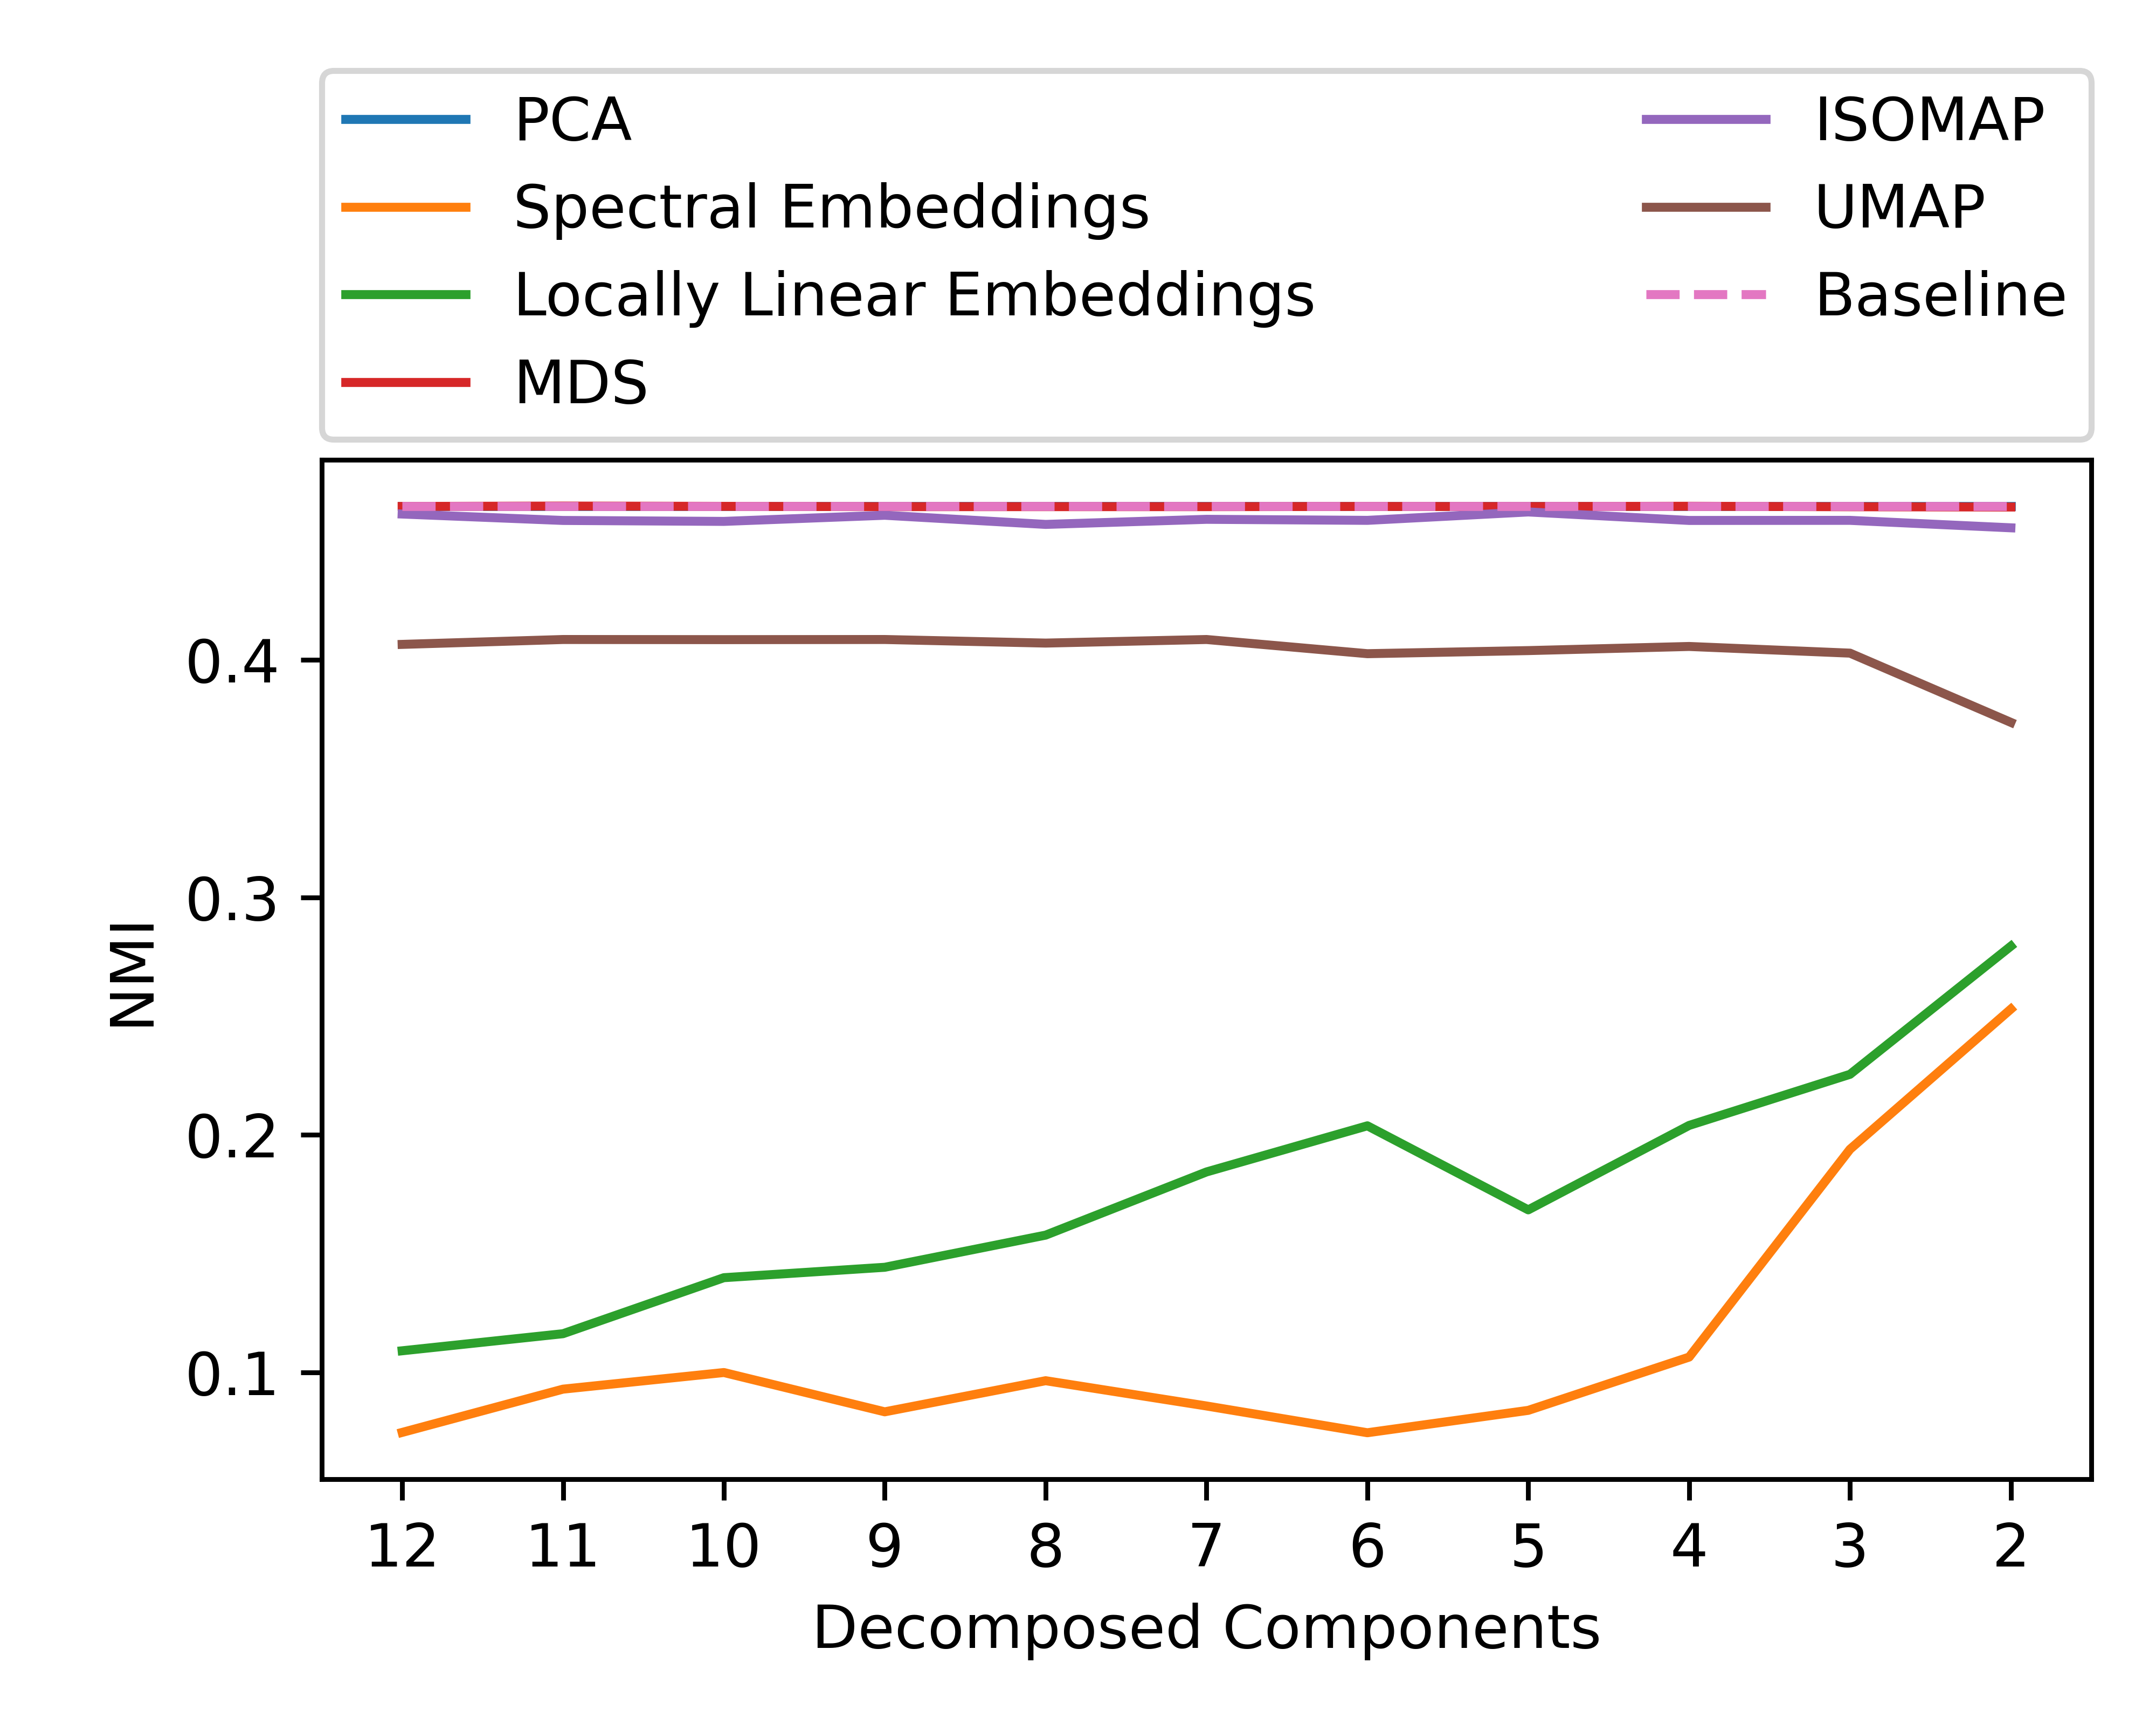
\includegraphics[width=0.48\linewidth]{images/charts_real/real_data_wine_nmi.png}
                        \label{subfig:wine:nmi}
                    }
                    \subfigure[]{
                        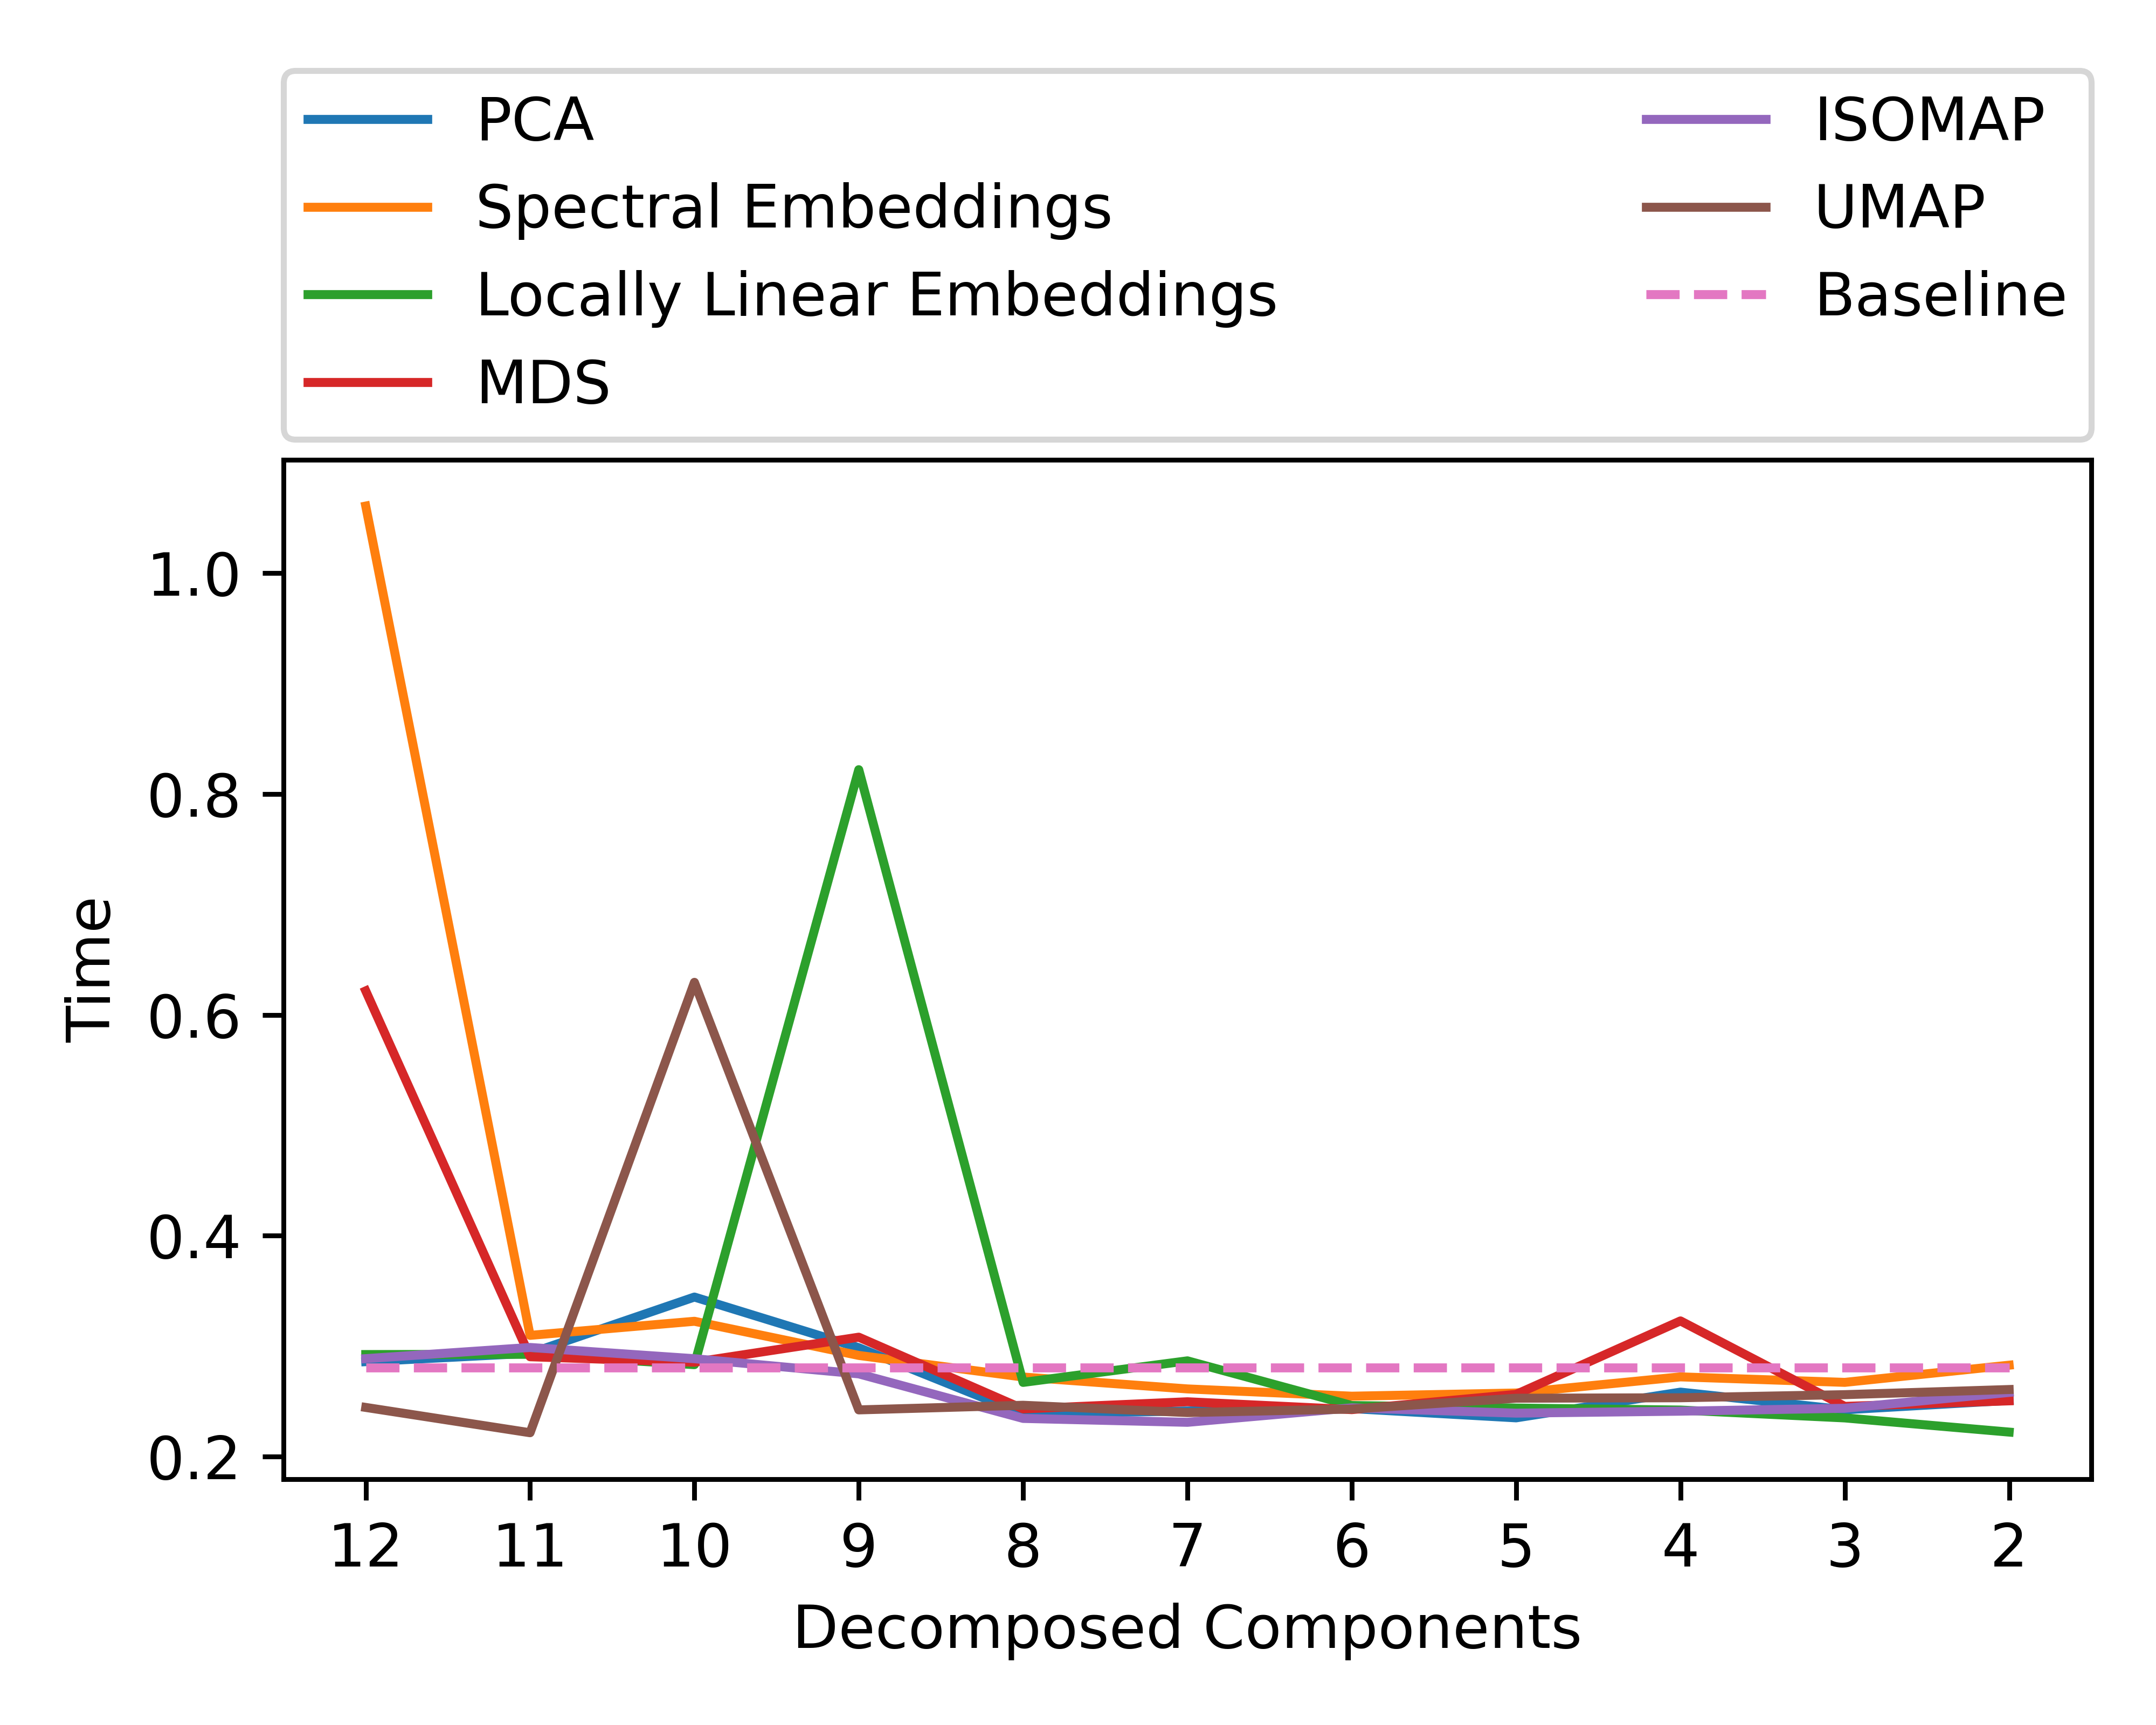
\includegraphics[width=0.48\linewidth]{images/charts_real/real_data_wine_time.png}
                        \label{subfig:wine:time}
                    }
                    \caption{Анализ влияния различных методов снижения размерности данных на кластеризацию набора данных Wine. Линия Baseline -- результат работы алгоритма \kmeans{} без предварительного снижения размерности. Результаты для
                        \subref{subfig:wine:ami} AMI;
                        \subref{subfig:wine:ari} ARI;
                        \subref{subfig:wine:nmi} NMI, а также на время работы алгоритма \subref{subfig:wine:time}.
                    }
                    \label{fig:wine}
                \end{figure}

                На рисунке \ref{fig:wine} представлены результаты экспериментов по кластеризации с предварительным снижением размерности на наборе данных Wine. Анализ показал, что методы PCA, ISOMAP и UMAP обеспечивают устойчивое поведение метрик, оставаясь на уровне или вблизи базовой линии на всем диапазоне компонент. Однако, несмотря на эту стабильность, они не продемонстрировали прироста качества кластеризации при уменьшении размерности. В то же время, методы Locally Linear Embedding (LLE) и Spectral Embedding показали заметное улучшение показателей AMI, ARI и NMI при переходе к малым числам компонент (2–4). Это указывает на их способность извлекать более информативную структуру данных в условиях значительного снижения размерности. Тем не менее, даже при росте метрик, их абсолютные значения остаются ниже по сравнению с другими методами, что ограничивает их практическую эффективность в этом конкретном примере. Важно отметить интересную закономерность: как ISOMAP, так и UMAP демонстрируют снижение качества кластеризации при переходе к размерностям, меньшим, чем реальное количество классов в выборке. Это может быть связано с потерей кластерной структуры, <<неукладывающейся>> в сжатое пространство. Такая деградация указывает на важность учета семантической емкости признакового пространства при выборе числа компонент. По времени выполнения алгоритма наилучшую стабильность и скорость показали MDS и PCA, что делает их предпочтительными с точки зрения вычислительной эффективности, особенно в сценариях, где время критично.


        \subsubsection{Сравнение методов снижения размерности}

\section{Заключение}
    В ходе учебной практики были достигнуты все поставленные цели и задачи. Был разработан подход применения алгоритмов снижения размерности в качестве этапа предобработки данных для кластеризации, проведена серия экспериментов, проанализированы результаты, которые будут использованы в дипломной работе.
